\documentclass[12pt]{article}
\usepackage[utf8]{inputenc}
\usepackage[colorlinks=true,linkcolor=blue,urlcolor=black,bookmarksopen=true]{hyperref}
\usepackage[margin=1in]{geometry}
\usepackage{graphicx}
\usepackage{tikz}
\usepackage{pst-plot}
\usepackage{mathtools}  
\usepackage{xcolor}
\usepackage{pgfplots}
\usepackage{amsmath,amssymb,amsfonts}
\usepackage{forest}
\usepackage{enumitem}
\usepackage{pgf-pie}  
\usepgfplotslibrary{statistics}

\graphicspath{ {./Images/} }
\pgfplotsset{compat = newest}

\title{Mathe Matura Kurs Mitschriften 
\break 1.Februar - 28.Dezember}
\author{Fabian Klaffenböck}
\date{\today}

\DeclareMathOperator{\e}{\mathrm{e}}

\begin{document}
%%% START MACRO %%%
\newcommand{\slopeTriangle}[5]
{
    % #1. Relative offset in x direction.
    % #2. Width in x direction, so xA-xB.
    % #3. Relative offset in y direction.
    % #4. Slope dydx.
    % #5. Plot options.

    \pgfplotsextra
    {
        \pgfkeysgetvalue{/pgfplots/xmin}{\xmin}
        \pgfkeysgetvalue{/pgfplots/xmax}{\xmax}
        \pgfkeysgetvalue{/pgfplots/ymin}{\ymin}
        \pgfkeysgetvalue{/pgfplots/ymax}{\ymax} 

        % Calculate auxilliary quantities.
        \pgfmathsetmacro{\xA}{\xmin+(#1+#2)*(\xmax-\xmin)}
        \pgfmathsetmacro{\yA}{\ymin+#3*(\ymax-\ymin)}
        \pgfmathsetmacro{\xB}{\xmin+#1*(\xmax-\xmin)}
        \pgfmathsetmacro{\yB}{\yA}
        \pgfmathsetmacro{\xC}{\xA}
        \pgfmathsetmacro{\yC}{\yA+(\xA-\xB)*#4}

        % Define coordinates for \draw.
        \coordinate (A) at (axis cs:\xA,\yA);
        \coordinate (B) at (axis cs:\xB,\yB);
        \coordinate (C) at (axis cs:\xC,\yC);

        % Draw slope triangle.
        \draw[#5]   (A)-- node[pos=0.5,anchor=north] {1}
                    (B)-- 
                    (C)-- node[pos=0.5,anchor=west] {#4}
                    cycle;
    }
}


\pgfmathdeclarefunction{gauss}{2}{%
  \pgfmathparse{1/(#2*sqrt(2*pi))*exp(-((x-#1)^2)/(2*#2^2))}%
}

%%% END MACRO %%%

\begin{titlepage}
    \maketitle
\end{titlepage}

\section{Zahlenmengen}

\hfill \break
Wichtige Symbole;
\begin{itemize}
    \item nur positive Zahlen und Null:  $\mathbb{Z}_0^{+}$
    \item nur negative Zahlen und Null: $\mathbb{Z}_0^{-}$
    \item nur positive Zahlen: $\mathbb{Z}^{+}$
    \item nur negative Zahlen: $\mathbb{Z}^{-}$
    \item Element von: $11-15 = -4 \in \mathbb{Z}$
    \item kein Element von: $11-15 = -4 \notin \mathbb{N}$
\end{itemize}

Diagramm der Zahlenmengen:\\
\hfill \break
\includegraphics[scale=0.4]{Zahlenmengen}

\break
\subsection{Die Natürlichen Zahlen}
Symbol: $\mathbb{N}$\\
sind alle Ganzen Positiv Zahlen

\hfill \break
\hfill \break
$ \mathbb{N}=\{0,1,2,3,4,5,6,\ldots\} $

\hfill \break
$ \mathbb{N}^{*}=\{0,1,2,3,4,5,6,\ldots\} $

\hfill \break
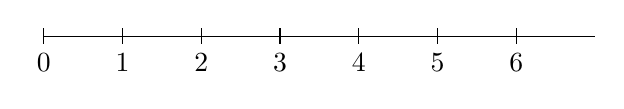
\begin{tikzpicture}
    \draw (0,0) -- (7,0);
    \foreach \X in {0,...,6}
    \draw (\X,0.1) -- (\X,-0.1);
    \foreach \X in {0,1,2,3,4,5,6}
    \node[anchor=north] at (\X,-0.1){\X};
\end{tikzpicture}

\hfill \break
Möglichkeiten mit den Natürlichen Zahlen:
\begin{enumerate}
    \item Addieren ist uneingeschränkt möglich:
          \begin{itemize}
              \item 1+3 = 4
              \item 10+5 = 15
          \end{itemize}
    \item Subtrahieren ist nur eingeschränkt möglich:
          \begin{itemize}
              \item 1-3 = ?
              \item 10-5 = 5
          \end{itemize}
    \item Multiplizieren ist uneingeschränkt möglich:
          \begin{itemize}
              \item 1*3 = 3
              \item 10*5 = 50
          \end{itemize}
    \item Dividieren ist nur eingeschränkt möglich:
          \begin{itemize}
              \item 1/3 = ?
              \item 10/5 = 2
          \end{itemize}
\end{enumerate}
\break
\subsection{Die Ganzen Zahlen}
Symbol: $\mathbb{Z}$\\
sind alle Ganzen Zahlen Positiv als auch Negatiev

\hfill \break
\hfill \break
$ \mathbb{Z}=\{\ldots,-3,-2,-1,0,1,2,3,\ldots\} $

\hfill \break
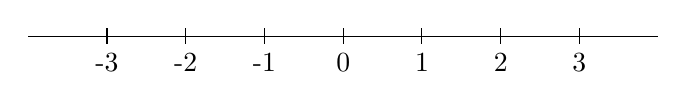
\begin{tikzpicture}
    \draw (-4,0) -- (4,0);
    \foreach \X in {-3,...,3}
    \draw (\X,0.1) -- (\X,-0.1);
    \foreach \X in {-3,-2,-1,0,1,2,3}
    \node[anchor=north] at (\X,-0.1){\X};
\end{tikzpicture}

\hfill \break
Möglichkeiten mit den Ganzen Zahlen:
\begin{enumerate}
    \item Subtrahieren ist uneingeschränkt möglich:
          \begin{itemize}
              \item 1-3 = -2
              \item 10-5 = 5
          \end{itemize}
    \item Dividieren ist nur eingeschränkt möglich:
          \begin{itemize}
              \item 1/3 = ?
              \item 10/5 = 2
          \end{itemize}
\end{enumerate}
\break
\subsection{Die Ratiaonalen Zahlen}
Symbol: $\mathbb{Q}$\\
sind die Menge aller Brüche

\hfill \break
\hfill \break
$ \mathbb{Q}=\{\frac{2}{3},\frac{7}{6},\frac{1}{6},1\frac{6}{7},0.125,0.\overline{3},\ldots\} $

\hfill \break
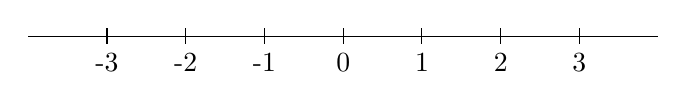
\begin{tikzpicture}
    \draw (-4,0) -- (4,0);
    \foreach \X in {-3,...,3}
    \draw (\X,0.1) -- (\X,-0.1);
    \foreach \X in {-3,-2,-1,0,1,2,3}
    \node[anchor=north] at (\X,-0.1){\X};
\end{tikzpicture}

\hfill \break
Benennung: 1/3 = $\frac{1}{3} = 0.\overline{3}$
\begin{itemize}
    \item 1 = Zähler, er zählt wie oft die Basis vorhanden ist
    \item 3 = Nenner, er gibt die Basis an
\end{itemize}

\hfill \break
Es bibt endliche und unendliche Dezimalzahlen:
\begin{itemize}
    \item endliche: 0.25
    \item unendliche: $0.\overline{25}$
\end{itemize}

\hfill \break
Möglichkeiten mit den Ganzen Zahlen:
\begin{enumerate}
    \item Dividieren ist ist uneingeschränkt möglich:
          \begin{itemize}
              \item 1/3 = $0.\overline{3}$
              \item 10/5 = 2
          \end{itemize}
\end{enumerate}

\hfill \break
Bekannte Büche:
\begin{itemize}
    \item $\frac{1}{5} = 0.2$
    \item $\frac{1}{4} = 0.25$
    \item $\frac{1}{2} = 0.5$
    \item $\frac{1}{8} = 0.125$
    \item $\frac{1}{9} = 0.\overline{1}$
    \item $\frac{1}{3} = 0.\overline{3}$
\end{itemize}
\break
\subsection{Die Reellen Zahlen}
Symbol: $\mathbb{R}$\\
sind alle Rationalen und irrationalen Zahlen

\hfill \break
Intervale beschreiben einen Zahlenbereich: $\{[1,2];[1.2,3.4]\}$


\hfill \break
\begin{tikzpicture}
    \draw (0,0) -- (4,0);
    \foreach \X in {1,...,3}
    \draw (\X,0.1) -- (\X,-0.1);
    \foreach \X in {1,3}
    \node[anchor=north] at (\X,-0.1){\X};
\end{tikzpicture}

\hfill \break
Zwischen 1 und 3 Liegen unendlich viele Zahlen


\hfill \break
Schreibweisen von Intervalen:
\begin{itemize}
    \item $[1,2]$ = Geschlossener Interval
    \item $[1,2) = [1,2[$ = Halboffener Interval
    \item $(1,2] = ]1,2]$ = Halboffener Interval
    \item $(1,2) = ]1,2[$ = Offener Interval
\end{itemize}



\hfill \break
Beschreibungen:
\begin{center}
    \begin{tabular}{ |c|c|c| }
        \hline
        Aufzählend             & Grafisch                                      & Beschreibend     \\
        A = $\{2,3,4,5\} $     & 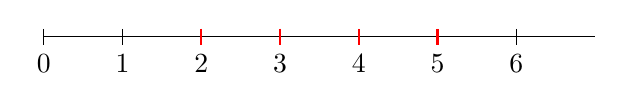
\begin{tikzpicture}
                                     \draw (0,0) -- (7,0);
                                     \foreach \X in {0,...,6}
                                     \draw (\X,0.1) -- (\X,-0.1);
                                     \foreach \X in {0,...,6}
                                     \node[anchor=north] at (\X,-0.1){\X};
                                     \foreach \X in {2,3,4,5}
                                     \draw[color=red,thick] (\X,0.1) -- (\X,-0.1);
                                 \end{tikzpicture} & A = $\{x \in \mathbb{N} | 2 \leq x \leq 5\}$ \\
        B = $\{-2,-1,0,1,2\} $ & 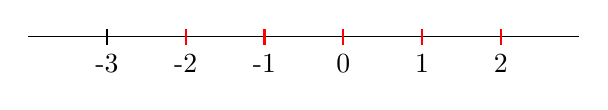
\begin{tikzpicture}
                                     \draw (-4,0) -- (3,0);
                                     \foreach \X in {-3,...,2}
                                     \draw (\X,0.1) -- (\X,-0.1);
                                     \foreach \X in {-3,...,2}
                                     \node[anchor=north] at (\X,-0.1){\X};
                                     \foreach \X in {-2,...,2}
                                     \draw[color=red,thick] (\X,0.1) -- (\X,-0.1);
                                 \end{tikzpicture} & B = $\{x \in \mathbb{Z} |-2 \leq x < 2\}$    \\
        C = $[-1,3]$           & 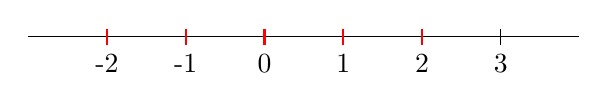
\begin{tikzpicture}
                                     \draw (-3,0) -- (4,0);
                                     \foreach \X in {-2,...,3}
                                     \draw (\X,0.1) -- (\X,-0.1);
                                     \foreach \X in {-2,...,3}
                                     \node[anchor=north] at (\X,-0.1){\X};
                                     \foreach \X in {-2,...,2}
                                     \draw[color=red,thick] (\X,0.1) -- (\X,-0.1);
                                 \end{tikzpicture} & C = $\{x \in \mathbb{R} |-1 \leq x < 3\}$    \\
        D = $]2,5]$            & 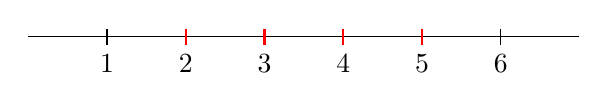
\begin{tikzpicture}
                                     \draw (0,0) -- (7,0);
                                     \foreach \X in {1,...,6}
                                     \draw (\X,0.1) -- (\X,-0.1);
                                     \foreach \X in {1,...,6}
                                     \node[anchor=north] at (\X,-0.1){\X};
                                     \foreach \X in {2,...,5}
                                     \draw[color=red,thick] (\X,0.1) -- (\X,-0.1);
                                 \end{tikzpicture} & D = $\{x \in \mathbb{R} | 2 < x \leq 5\}$    \\
        \hline
    \end{tabular}
\end{center}



\break
\section{Rechenregeln}

\hfill \break
\subsection{Addition}

$$Addition: 3+7=10$$
$$Addition: Summand+Summand=Summe$$
Die Summanden sind vertauschbar (Kommutativgesetz)
\hfill \break
\subsection{Subtraktion}

$$Subtraktion: 10-7=3$$
$$Subtraktion: Minuend-Subtrahend=Differenz$$
Minuend und Subtrahend sind nicht vertauschbar
\hfill \break
\subsection{Multiplikation}

$$Multiplikation: 8*2=16$$
$$Multiplikation: Faktor*Faktor=Produkt$$
Die Faktoren sind vertauschbar (Kommutativgesetz)
\hfill \break
\subsection{Division}

$$Division: 16/2=8$$
$$Division: Divident/Divisor=Quotient$$
Divident und Divisor sind nicht vertauschbar
\hfill \break
\newpage
\subsection{Prozentrechnung}

\begin{itemize}
    \item \% = Zerlegung in 100 Teile
    \item 1\% = 1 Teil von 100
    \item 5\% = 5 Teile von 100
    \item p\% = p Teile von 100
    \item P = Prozentwert
    \item G = Grundwert
\end{itemize}

\hfill \break
$$\frac{G}{100}*P = \frac{p}{100}*G = A$$


\hfill \break
Example:\\
{\setlength{\fboxrule}{0.8pt}
\fcolorbox{black}{lightgray}{10\% von 130\texteuro = $\frac{130}{100}$*10 =13\texteuro }}

\hfill \break
Example:\\
\fboxrule=0.8pt \fcolorbox{black}{lightgray}{%
    \begin{tabular}[t]{@{}l@{}}
        $A=\frac{p}{100}*G$           \\
        $13=\frac{p}{100}*130$ / *100 \\
        $P=10=\frac{130}{13}$
    \end{tabular}}\\
\medskip

\hfill \break
Änderungsfaktor:
\begin{itemize}
    \item $\Rightarrow$ Vermehrung um 5\% $\Rightarrow$ 105\% = 1,05
    \item $\Rightarrow$ Verminderung um 5\% $\Rightarrow$ 95\% = 0,95
\end{itemize}
\medskip
Example:\\
\fboxrule=0.8pt \fcolorbox{black}{lightgray}{%
    \begin{tabular}[t]{@{}l@{}}
        $300*1,06 = 318$
    \end{tabular}}
\hfill \break
\newpage
\subsection{Vorrangregeln}

\textcolor{red}{Kla}mmer vor \textcolor{red}{Pu}nkt vor \textcolor{red}{Stri}ch - Rechnung\\
\textcolor{red}{KlaPuStri - Regel}\\

\hfill \break
Weitere Klammern (es wird von innen nach außen gerechnet): $\{\}$,$[]$,()

\hfill \break
Example:\\
\fboxrule=0.8pt \fcolorbox{black}{lightgray}{%
    \begin{tabular}[t]{@{}l@{}}
        (3+4)*2-1 = \\
        (7)*2-1 =   \\
        14-1 = 13
    \end{tabular}}\\
\hfill \break
\subsection{Potenzen}

\begin{huge}
    $a^n$
\end{huge}

\begin{itemize}
    \item Alles zusammen wird als Potenz bezeichnet
    \item a wird als Basis bezeichnet
    \item n wird als Exponent bezeichnet
\end{itemize}

\hfill \break
Example:\\
\fboxrule=0.8pt \fcolorbox{black}{lightgray}{%
    \begin{tabular}[t]{@{}l@{}}
        $10^2 = $ = 10*10 = 100                \\
        $10^3 = $ = 10*10*10 = 1000            \\
        $(-5)^3$ = $(-5)$*$(-5)$*$(-5)$ = -125 \\
        $(-2)^4$ = $(-2)$*$(-2)$*$(-2)$*$(-2)$ = 16
    \end{tabular}}\\


\hfill \break
Ist die Basis eine negative Zahl und der Exponent,...\\
\begin{tabular}[t]{@{}l@{}}
    ...Gerade so ist das Ergebnis positiv. \\
    ...ungerade so ist das Ergebnis negativ.
\end{tabular}
\hfill \break
\newpage
\subsection{Rechnen mit ganzen Zahlen}

Regeln:\\
\begin{itemize}
    \item (+)(+) = +
    \item (-)(-) = +
    \item (-)(+) = -
    \item (+)(-) = -
\end{itemize}

\hfill \break
Example:\\
\fboxrule=0.8pt \fcolorbox{black}{lightgray}{%
    \begin{tabular}[t]{@{}l@{}}
        $(-4)+(-2)-(+5)-(-1) = ? $ \\
        $-4-2-5+1 = -10$          \\
    \end{tabular}}
\hfill \break
\subsection{Betrag}

Betrag: $\vert-2 \vert = 2$\\
Das Zeichen $\vert$ ist der Betragsstrich\\
Der Betrag ist immer eine positive Zahl.\\

\hfill \break
Example:\\
\fboxrule=0.8pt \fcolorbox{black}{lightgray}{%
    \begin{tabular}[t]{@{}l@{}}
        $\vert-2-1\vert = \vert-3\vert = 3$
    \end{tabular}}\\


\hfill \break
\newpage
\subsection{Teilbarkeitsregeln}

Regeln:
\begin{itemize}
    \item Eine Zahl ist durch 2 teilbar, wenn sie gerade ist, also ihre letzte Ziffer eine 2,4,6,8 oder O ist.
    \item Eine Zahl ist durch 3 teilbar, wenn ihre Quersumme, also die Summe all ihrer Ziffern durch 3 teilbar ist.
    \item Eine Zahl ist durch 4 teilbar, wenn ihre letzten 2 Stellen durch 4 teilbar sind.
    \item Eine Zahl ist durch 5 teilbar, wenn ihre letzte Stelle eine 5 oder eine O ist.
    \item Eine Zahl ist durch 6 teilbar, wenn sie durch 2 und durch 3 teilbar ist, also wenn sie gerade ist und ihre Quersumme durch 3 teilbar ist.
    \item Eine Zahl ist durch 8 teilbar, wenn ihre letzten 3 Stellen durch 8 teilbar sind.
    \item Eine Zahl ist durch 9 teilbar, wenn ihre Quersumme durch 9 teilbar ist.
    \item Eine Zahl ist durch 10 teilbar, wenn ihre letzte Stelle eine ist. OD
    \item Eine Zahl ist durch 12 teilbar, wenn sie durch 3 und durch 4 teilbar ist.
    \item Eine Zahl ist durch 15 teilbar, wenn sie durch 3 und durch 5 teilbar ist.
    \item Eine Zahl ist durch 18 teilbar, wenn sie durch 2 und durch 9 teilbar ist.
    \item Eine Zahl ist durch 20 teilbar, wenn ihre letzte Stelle eine O und ihre vorletzte Stelle gerade ist.
\end{itemize}
\hfill \break
\newpage
\subsection{logarithmen}

Rechenregeln:
\begin{itemize}
    \item $Log(b^x) = x*Log(b)$
    \item $Log(a*b) = Log(a)+Log(b)$
    \item $Log(\frac{a}{b}) = Log(a)-Log(b)$
    \item $Log(x) = \frac{Log_{10}(x)}{Log_{10}(x)}$
    \item $Log_5(5) = 1$
    \item $Log_{10}(10) = 1$
    \item $Log_e(e) = 1$
    \item $Log_a(a) = 1$
    \item $Log_e(e) = Ln(e)= 1$
    \item Elemente mit - kommen in den Nenner
    \item Elemente mit + kommen in den Zähler
\end{itemize}
\break
\section{Primzahlen}

\hfill \break
$P \subseteq \mathbb{N}$\\
$P = \{2,3,5,7,11,13,17,19,23,...\}$\\


Eigenschaften:
\begin{itemize}
    \item Primzahlen sind Zahlen, die nur durch Eins und durch sich selber teilbar sind.
    \item Die kleinste Primzahl ist Zwei.
\end{itemize}

\subsection{Primfaktorzerlegung}

\hfill \break
Es wird immer mit der kleisten Primzahl zerlegt.

\hfill \break
$12 = 4*3$\\
$12 = 2*2*3 = 2^2*3$\\

\hfill \break
\fboxrule=0.8pt \fcolorbox{lightgray}{lightgray}{%
    \begin{tabular}{ c|c}
        12 & 2 \\
        6  & 2 \\
        3  & 3 \\
        1  &   \\
    \end{tabular}}\\

\hfill \break
$180 = 4*9*5$\\
$180 = 2*2*3*3 = 2^2*3^2*5$\\

\hfill \break
\fboxrule=0.8pt \fcolorbox{lightgray}{lightgray}{%
    \begin{tabular}{ c|c }
        180 & 2 \\
        90  & 2 \\
        45  & 3 \\
        15  & 3 \\
        5   & 5 \\
        1   &   \\
    \end{tabular}}\\
\break
\newpage
\subsection{Größter gemeinsamer Teiler (ggt)}

Das GGT wird mittles Primfaktorzerlegung ermittelt.\\
Die Zahlen die in beiden Zerlegungen vorhanden sind werden Zusammen-multipliziert.\\

\hfill \break
Example: Ermittling des ggt von 36 und 60\\
\fboxrule=0.8pt \fcolorbox{lightgray}{lightgray}{%
    \begin{tabular}{ c|c||c|c}
        36 & \textcolor{red}{2}   & 60 & \textcolor{red}{2}   \\
        18 & \textcolor{green}{2} & 30 & \textcolor{green}{2} \\
        9  & \textcolor{blue}{3}  & 15 & \textcolor{blue}{3}  \\
        3  & 3                    & 5  & 5                    \\
        1  &                      & 1  &                      \\
    \end{tabular}}
$ggt(36,60) = \textcolor{red}{2}*\textcolor{green}{2}*\textcolor{blue}{3} = 12$
\break
\subsection{Kleinste gemeinsame Vielfache (kgv)}

\hfill \break
Das kgv wird errechnet in dem man jeden Faktor in der jeweils höchst vorkommenden Potenz miteinenader multipliziert.\\

\hfill \break
Das kgv wird wie folged berechnet:\\
\includegraphics[scale=0.8]{KGV}

\hfill \break
Example: Ermittling des kgv von 24 und 30\\
\fboxrule=0.8pt \fcolorbox{lightgray}{lightgray}{%
    \begin{tabular}{c|c||c|c}
        24 & 2 & 30 & 2 \\
        12 & 2 & 15 & 2 \\
        6  & 2 & 5  & 5 \\
        3  & 3 & 4  &   \\
        1  &   &    &   \\
    \end{tabular}}
$kgv(24,30) = 2^3*3^1*5^1 =120$



\break
\section{Brüche}

\hfill \break
Benennung: 1/3 = $\frac{1}{3} = 0.\overline{3}$
\begin{itemize}
    \item 1 = Zähler, er zählt wie oft die Basis vorhanden ist
    \item 3 = Nenner, er gibt die Basis an
\end{itemize}

\hfill \break
\subsection{Kürzen von Brüchen}

Der Wert eines Bruches bleibt gleich wen men Zähler und Nenner durch die selbe Zahl dividiert.

\hfill \break
Example: /10:
\fboxrule=0.8pt \fcolorbox{black}{lightgray}{%
    \begin{tabular}[t]{@{}l@{}}
        $\frac{30}{40} = \frac{3}{4}$ \\
    \end{tabular}}
    
\hfill \break   
Example: /8:
\fboxrule=0.8pt \fcolorbox{black}{lightgray}{%
    \begin{tabular}[t]{@{}l@{}}
        $\frac{24}{32} = \frac{3}{4}$ \\
    \end{tabular}}

\hfill \break
\subsection{Erweitern von Brüchen}

Der Wert eines Bruches bleibt gleich wen men Zähler und Nenner durch die selbe Zahl Multipliziert.

\hfill \break
Example: *90:
\fboxrule=0.8pt \fcolorbox{black}{lightgray}{%
    \begin{tabular}[t]{@{}l@{}}
        $\frac{1}{2} = \frac{90}{180}$ \\
    \end{tabular}}\\
Example: *50:
\fboxrule=0.8pt \fcolorbox{black}{lightgray}{%
    \begin{tabular}[t]{@{}l@{}}
        $\frac{2}{5} = \frac{100}{250}$ \\
    \end{tabular}}

\hfill \break
\subsection{Addieren von Brüchen}

Brüche werden Addieren in dem man sie auf gemeinsamen Nenner bring mit der methode des kgv.

\hfill \break
Example:
\fboxrule=0.8pt \fcolorbox{black}{lightgray}{%
    \begin{tabular}[t]{@{}l@{}}
        $\frac{1}{2} +\frac{1}{3} =\frac{3}{6} +\frac{2}{6} = \frac{5}{6}$ \\
    \end{tabular}}
\hfill \break
\subsection{Subtrahieren von Brüchen}

Brüche werden Subtrahiert in dem man sie auf gemeinsamen Nenner bring mit der Methode des kgv.

\hfill \break
Example:
\fboxrule=0.8pt \fcolorbox{black}{lightgray}{%
    \begin{tabular}[t]{@{}l@{}}
        $\frac{1}{6} -\frac{1}{8} =\frac{4}{24} +\frac{3}{24} = \frac{4-3}{24} = \frac{1}{24}$ \\
    \end{tabular}}
\hfill \break
\subsection{Multiplizieren von Brüchen}

Brüche werden Multipliziert in dem man Zähler mit Zähler und Nenner mit Nenner multipliziert.

\hfill \break
Example:
\fboxrule=0.8pt \fcolorbox{black}{lightgray}{%
    \begin{tabular}[t]{@{}l@{}}
        $\frac{6}{7} *\frac{1}{5} =\frac{6*1}{7*5} = \frac{6}{35}$ \\
        \hfill\\
        $5 *\frac{1}{2} =\frac{5*1}{1*2} = \frac{5}{2}$            \\
    \end{tabular}}
\hfill \break
\subsection{Dividieren von Brüchen}

Brüche werden Dividiert in dem man den Kehrwert des Divisors multipliziert.

\hfill \break
Example:
\fboxrule=0.8pt \fcolorbox{black}{lightgray}{%
    \begin{tabular}[t]{@{}l@{}}
        $\frac{16}{7} / \frac{8}{1} = \frac{16}{7} * \frac{1}{8} = \frac{2}{7}$ \\
    \end{tabular}}
\hfill \break
\subsection{Doppelbrüche}

Bei Doppelbrüchen werden die ausen und innenglieder miteinander Multipliziert.\\
Ausenglieder sind obern und Innenglieder sind innen.

\hfill \break
Example:
\fboxrule=0.8pt \fcolorbox{black}{lightgray}{%
    \begin{tabular}[t]{@{}l@{}}
        $\frac{\frac{4}{7}}{\frac{20}{21}} =\frac{4*21}{7*20} = \frac{1*3}{1*5} = \frac{3}{5}$ \\
    \end{tabular}}
\\

\break
\newpage
\section{Gleichungen}

\hfill \break
Wichtige Symbole:
\begin{itemize}
    \item $1=3\ f.A. = falsche aussage (f.A.)$
    \item $3=3\ w.A. = Ware aussage (w.A.)$
    \item 1. Binomische Formel = $(x+y)^2 = x^2+2xy+y^2$
    \item 2. Binomische Formel = $(x-y)^2 = x^2-2xy+y^2$
    \item 3. Binomische Formel = $(x+y)*(x-y) = x^2-y^2$
\end{itemize}

\hfill \break
Vorsilben:
\begin{itemize}
    \item $10^{-12} = piko = p $
    \item $10^{-9} = nano = n $
    \item $10^{-6} = mikro = \mu $
    \item $10^{-3} = mill = m$
    \item $10^{-2} = centi = c$
    \item $10^{-1} = dezi = d$
    \item $10^1 = Deka = da$
    \item $10^2 = Hekto = h$
    \item $10^3 = Kilo = k$
    \item $10^6 = Mega = M = 1 Milion$
    \item $10^9 = Giga = G = 1 Miliarde$
    \item $10^12 = Tera = T = 1 Bilion$
\end{itemize}


\break
\subsection{Einfache Gleichungen}

Ich denke mir eine Zahl, multipliziere sie mit 2 und subtrahiere anschliesend 1. Ich erhalte 15.

\hfill \break
Example:\\
\fboxrule=0.8pt \fcolorbox{lightgray}{lightgray}{%
    \begin{tabular}{ |c|}
        \hline
        $2x-1=15$ / +1 \\
        $2x=16$ / /2   \\
        $x=8$          \\
        \hline
    \end{tabular}}\\

\hfill \break
Example:\\
\fboxrule=0.8pt \fcolorbox{lightgray}{lightgray}{%
    \begin{tabular}{ |c|}
        \hline
        $(x-9)*4=100$ / Ausmultiplizieren \\
        $4x-36=100$ / +36                 \\
        $4x=136$ / /4                     \\
        $x=34$                            \\
        \hline
    \end{tabular}}\\

\hfill \break
Bei einem Minus vor der Klammer werden alle Vorzeichen in der Klammer vertauscht.\\
Example:\\
\fboxrule=0.8pt \fcolorbox{lightgray}{lightgray}{%
    \begin{tabular}{ |c|}
        \hline
        $3(x+4)-(x-8) = 6x-2(3+x)$ / Klammern auflösen \\
        $3x+12-x+8=6x-6-2x$ / Zusammenrechnen          \\
        $2x+20=4x-6$ / -2x                             \\
        $20=2x-6$ / +6                                 \\
        $26=2x$ / /2                                   \\
        $13=x$                                         \\
        $x=13$                                         \\
        \hline
    \end{tabular}}

\break
\newpage
\subsection{Gleitkommadarstellung}

\hfill \break
$2,731*10^3 = 2731$
\begin{itemize}
    \item $2,731$: Mantisse(m)
    \item $10^3$: Zehnerpotenz
\end{itemize}

\hfill \break
Bei einer positiven Hochzahl wird das Komma nach Rechts verschoben.\\

\hfill \break
Example:\\
\fboxrule=0.8pt \fcolorbox{lightgray}{lightgray}{%
    \begin{tabular}{|c|}
        \hline
        $12000000000000 = 1,2^{13}$ \\
        \hline
    \end{tabular}}\\
\hfill \break
Bei einer negativen Hochzahl wird das komma anch Links verschoben.\\

\hfill \break
Example:\\
\fboxrule=0.8pt \fcolorbox{lightgray}{lightgray}{%
    \begin{tabular}{ |c|}
        \hline
        $0,00000325 = 3,25^{-6}$ \\
        \hline
    \end{tabular}}\\
\break
\newpage
\subsection{Terme}

Ein Term ist ein sinvoller matehmatischer Ausdruck bestehend aus Zahlen,Variablen und Rechenzeichen.

\hfill \break
Benennung:
\begin{itemize}
    \item $2x$: Monom
    \item $2x-1$: Binom
    \item $x+y-z$: Trinom
    \item $x+y-z-4$: Polinom
\end{itemize}

\hfill \break
Example:\\
\fboxrule=0.8pt \fcolorbox{lightgray}{lightgray}{
    \begin{tabular}{c}
        $2x*(5y+3w) = 10xy+6xw$                  \\
        \hline
        $(x-2)*(x+5) = x^2+5x-2x-10 = x^2+3x-10$ \\
        \hline
        $(x+y)*(x+y) = x^2+2xy+y^2$              \\
    \end{tabular}}

\break
\hfill \break
\subsection{Gleichungen mit Brüchen}

\hfill \break
Example:\\
\fboxrule=0.8pt \fcolorbox{black}{lightgray}{%
    \begin{tabular}[t]{@{}l@{}}
        $\frac{x}{2} +\frac{x}{3} = 5$ /gemeinsamer Nenner ist 6 \\
        $\frac{3x+2x}{6} = 5$                                    \\
        $\frac{5x}{6} = 5$ / *6                                  \\
        $5x = 30$ / /5                                           \\
        $x = 6$                                                  \\
    \end{tabular}}\\

\hfill \break
Example:\\
\fboxrule=0.8pt \fcolorbox{black}{lightgray}{%
    \begin{tabular}[t]{@{}l@{}}
        $\frac{2x}{3} -\frac{x}{4} = \frac{5}{6}$ /gemeinsamer Nenner ist 12 \\
        \hfill                                                               \\
        $\frac{8x-3x}{12} = \frac{10}{12}$                                   \\
        \hfill                                                               \\
        $\frac{5x}{12} = \frac{10}{12}$ / *12                                \\
        $5x = 10$ / /5                                                       \\
        $x = 2$                                                              \\
    \end{tabular}}
\break
\newpage
\subsection{Formelumformen}

\hfill \break
Example auflösen nach $k$:\\
\fboxrule=0.8pt \fcolorbox{black}{lightgray}{%
    \begin{tabular}[t]{@{}l@{}}
        $-8=4k$  / /4 \\
        $-2=k$        \\
    \end{tabular}}

\hfill \break
Example auflösen nach $d$:\\
\fboxrule=0.8pt \fcolorbox{black}{lightgray}{%
    \begin{tabular}[t]{@{}l@{}}
        $6=(-1)*(-2)+d$ \\
        $6=2+d$ /-2     \\
        $d=4$           \\
    \end{tabular}}

\hfill \break
Example auflösen nach $k$:\\
\fboxrule=0.8pt \fcolorbox{black}{lightgray}{%
    \begin{tabular}[t]{@{}l@{}}
        $\frac{1}{e}=\frac{1}{g}+\frac{1}{k}$ / auf gemeisamen Nenner bringen (egk) \\
        $\frac{gk}{egk}=\frac{ek+eg}{egk}$ /*egk                                    \\
        $gk=ek+eg$ /-ek                                                             \\
        $gk-ek=eg$                                                                  \\
        $k*(g-e)=eg$ //(e-g)                                                        \\
        $k=\frac{eg}{g-e}$                                                          \\
    \end{tabular}}

\hfill \break
Example auflösen nach $m$:\\
\fboxrule=0.8pt \fcolorbox{black}{lightgray}{%
    \begin{tabular}[t]{@{}l@{}}
        $m=\frac{1-k}{b+k}$ /*(b+k) \\
        $m*(b+k)=1-k$               \\
        $mb+mk=1-k$ /-1\ /-mk       \\
        $mb-1=k-mk$                 \\
        $mb-1=k*(-1-mk)$            \\
        $k=\frac{mb-1}{1-(1+m)}$    \\
        $k=\frac{1-md}{m+1}$        \\
    \end{tabular}}\\
\break
\newpage
\subsection{PQ und ABC Formel}


Um die abc-Formel anwenden zu können, müssen wir die quadratische Gleichung in die allgemeine Form überführen, das heißt dort muss $irgendwas = 0$ stehen. Liegt diese dann vor, können wir die abc-Formel direkt anwenden.
Sind 3 Terme vorhanden sprechen wir von der ABC Formel, wen nur 2 Terme vorhanden sind handelt es sich um die PQ Formal.
Diese kamm mit der ABC Formel leböst werden indem man die Fehlenden Terme mit 1 ersetzt.\\

\hfill \break
Example:\\
\fboxrule=0.8pt \fcolorbox{lightgray}{lightgray}{%
    \begin{tabular}{ |c|}
        \hline
        $3*x^2 + 3*x = 18$                                                                      \\
        $3*x^2 + 3*x = 18$  /-18                                                                \\
        $3*x^2 + 3*x - 18 = 0$                                                                  \\
        \\
        Nun wird die obige Formel herangezogen und eingesetzt. Es ist a = 3, b = 3 und c = -18. \\
        \\
        $x_{1,2} = \frac{-b\pm \sqrt{b^2-4*a*c}}{2*a}$  /a=3, b=3, c=-18                        \\
        \\
        $x_{1,2} = \frac{-3 \pm \sqrt{3^2 - 4*3*(-18)}}{2*3}$                                   \\
        \\
        $x_{1,2} = \frac{-3\pm\sqrt{9+216}}{6} $                                                \\
        \\
        $x_{1,2} = \frac{-3\pm\sqrt{225}}{6}$                                                   \\
        \\
        $x_{1,2} =\frac{-3\pm15}{6}$                                                            \\
        \\
        $x_1 = \frac{-3+15}{6} = \frac{12}{6} = 2$                                              \\
        \\
        $x_2 = \frac{-3-15}{6} = \frac{-18}{6} = -3$                                            \\
        \hline
    \end{tabular}}

\newpage
\hfill \break
Rechnungsweg im Taschenrechner $TI-82STATS$:\\
\begin{itemize}
    \item Wenn die ABC-Formel schon im Taschenrechner gespeichert ist:
    \item Taste $PRGM$
    \item ABC-Funktion auswählen
    \item $ENTER$ Taste
    \item Wenn nacheinander die Buchstaben A-B-C, erscheinen dann den entsprechenden Wert eintragen (Bei einer negativen Zahl das Vorzeichen verwenden und nicht das Rechenzeichen !!!)
    \item Danach erscheinen untereinander 2 Zahlen. Das sind die beiden Lösungen.
    \item Wenn die ABC-Formel noch nicht im Taschenrechner gespeichert ist, muss diese erst eingespeichert werden...
\end{itemize}

\break
\newpage
\subsection{Sätze von Vietá}

\hfill \break
Die Sätze von Vietá werden verwendet um $p$ und $q$ zu errechnen.

\hfill \break
\begin{itemize}
    \item (1.): $(x-x_1)*(x-x_2) = 0$
    \item (2.): $x_1*x_2 = q$
    \item (3.): $x_1+x_2 = -p$ oder $-(x_1+x_2) = p$
\end{itemize}

\hfill \break
Example:\\
\fboxrule=0.8pt \fcolorbox{lightgray}{lightgray}{%
    \begin{tabular}{ |c|}
        \hline
        $(x-3)*(x+7)=0$ \\
        $\Downarrow \Downarrow $ \\
        $x_1 = 3$    $x_2 = -7$ \\
        $x^2-3x+7x-21=0$\\
        $x^2+4x-21=0$\\
        $\Downarrow$\\
        $x^2+4x-21=0$\\
        $x^2+px+q=0$\\
        \hline
    \end{tabular}}
\break
\newpage
\subsection{Die Diskreminanten}

\hfill \break
Die Diskreminante gibt an wie viele Lösungen es in einer Quadratischen Gleichung gibt.
\hfill \break

Example:\\
\fboxrule=0.8pt \fcolorbox{lightgray}{lightgray}{%
    \begin{tabular}{c|c|c}
        $4x^2+x+10=0$                                & $4x^2-12x+9=0$                              & $2x^2+3x-20=0$                             \\
        \\
        $1X_2 = \frac{-1 \pm \sqrt{1-4*4*10}}{2*4} $ & $1X_2 = \frac{12 \pm \sqrt{144-4*4*9}}{8} $ & $1X_2 = \frac{-3 \pm \sqrt{9+4*2*20}}{4} $ \\
        \\
        $1X_2 = \frac{-1 \pm \sqrt{-159}}{2*4} $ & $1X_2 = \frac{12 \pm \sqrt{0}}{8} $         & $1X_2 = \frac{-3 \pm 13}{4} $              \\
        \\
        $ $                                          & $X_1= \frac{12}{8}= \frac{3}{2} $           & $X_1 =2.5  X_2 = -4 $                      \\
        $ D<0$                                       & $D=0 $                                      & $D>0 $                                     \\
        Keine Lösung                                 & Eine Lösung                                 & Zwei Lösungen                              \\
    \end{tabular}}
\break
\newpage
\subsection{Wurzelgleichungen}

\hfill \break
Von einer Wurzelgleichung spricht man wen Teile der Gleichung unter einer Wurzel stehen.
Die Probe ist Umungänglich da durch das Quadrieren (da das keine Eqivalenzumformung ist) eine "falsche Lösung" entstehen kann.

\hfill \break
Example einfache Wurzelgleichungen:\\
\fboxrule=0.8pt \fcolorbox{black}{lightgray}{%
    \begin{tabular}[t]{@{}l@{}}
        Rechnung:                 \\
        $\sqrt{2x+3} = 5$ // $^2$ \\
        $2x+3 = 25$ // $-3$       \\
        $2x = 22$ // $/2$         \\
        $x = 11$                  \\
        \\
        Probe:                    \\
        $\sqrt{2*11+3} = 5$       \\
        $\sqrt{25} = 5$           \\
        $5 = 5 = w.A.$            \\
    \end{tabular}}

\hfill \break
Example Wurzelgleichung mit Binomischer Formel:\\
\fboxrule=0.8pt \fcolorbox{black}{lightgray}{%
    \begin{tabular}[t]{@{}l@{}}
        Rechnung:                            \\
        $\sqrt{2x+7} = \sqrt{x+3}+1$ // $^2$ \\
        $2x+7 = (x+3)+2*1*\sqrt{x+3}+1$      \\
        $2x+7 = x+4+2*\sqrt{x+3}$ // $-x-4$  \\
        $x+3 = 2\sqrt{x+3}$ // $^2$          \\
        $x^2+6x+9 = 4x+12$ //$-4x-12$        \\
        $x^2+2x-3 = 0$                       \\
        $x_1 = 1$                            \\
        $x_2 = -3$                           \\
        \\
        Probe  1:                            \\
        $\sqrt{2-7} = \sqrt{1-3}+1$          \\
        $3 = 3 = w.A.$                       \\
        \\
        Probe  2:                            \\
        $\sqrt{-6+7} = \sqrt{-3+3}+1$        \\
        $1 = 1 = w.A.$                       \\
    \end{tabular}}
\break
\newpage
\subsection{Teilweises Wurzelziehen und Bruchschreibweise}


\hfill \break
Beim teilweisen Wurzelziehen wird nur von einem Faktor die Wurzel gezogen. Der andere Faktor bleib unter der Wurzel stehen.\\

\hfill \break
Regeln:\\
\begin{itemize}
    \item $\sqrt{a}* \sqrt{b} = \sqrt{ab}$
    \item $\sqrt[n]{a}* \sqrt[n]{b} = \sqrt[n]{ab}$
    \item $\sqrt{9}+ \sqrt{16} \neq  \sqrt{9+16}$
    \item $3+5 \neq 5$
    \item $\frac{\sqrt[n]{a}}{\sqrt[n]{b}} = \sqrt[n]{\frac{a}{b}}$
    \item $a^\frac{r}{s} \Leftrightarrow  \sqrt[s]{a^r}$
    \item $a^{-\frac{r}{s}} \Leftrightarrow  \frac{1}{\sqrt[s]{a^r}}$
\end{itemize}

\hfill \break
Example:\\
\fboxrule=0.8pt \fcolorbox{black}{lightgray}{%
    \begin{tabular}[t]{@{}l@{}}
        $\sqrt{12} = \sqrt{4} * \sqrt{3} = 2* \sqrt{3}$      \\
        $\sqrt{50} = \sqrt{25} * \sqrt{2} = 5* \sqrt{2}$     \\
        $\sqrt{18} = \sqrt{9} * \sqrt{2} =3* \sqrt{2}$       \\
        \\
        $\sqrt[2]{a^2} = a$                                  \\
        $\sqrt[2]{a^3} = a*\sqrt{2}$                         \\
        $\sqrt[2]{a^5} = a^2*\sqrt{2}$                       \\
        $\sqrt{50*a^4*b^5*c^7} = 5*a^2*b^2*c^3*\sqrt{2*b*c}$ \\
        \\
        $a^\frac{2}{5} = \sqrt[5]{a^2}$                      \\
        $a^{-\frac{3}{7}} = \frac{1}{\sqrt[7]{a^3}}$         \\
    \end{tabular}}
\break
\newpage
\subsection{Matrizen rechnen}

\hfill \break
Eine Matrix (Gleichungssysteme mit 3 Unbekannten), die aus $m$ Zeilen und $n$ Spalten besteht, hat die Dimension $m\times$.

\hfill \break
\[
    A_{m\times n} =
    \left[ {\begin{array}{cccc}
                    a_{11} & a_{12} & \cdots & a_{1n} \\
                    a_{21} & a_{22} & \cdots & a_{2n} \\
                    \vdots & \vdots & \ddots & \vdots \\
                    a_{m1} & a_{m2} & \cdots & a_{mn} \\
                \end{array} } \right]
\]

\hfill \break
Example:\\
\fboxrule=0.8pt \fcolorbox{lightgray}{lightgray}{%
    \begin{tabular}{ |c|}
        \hline
        (1)$x+2y+3z=10$ \\
        (2)$2x+3y+z=13$ \\
        (3)$3x+y+2z=13$ \\
        \hline
    \end{tabular}}\\

\hfill \break
Rechenmatrix:
$\left(\begin{array}{cccc}
            1 & 2 & 3 \\
            2 & 3 & 1 \\
            3 & 1 & 2 \\
        \end{array}\right)$\\

\hfill \break
Lösung:
$\left(\begin{array}{ccccc}
            10 \\
            13 \\
            13 \\
        \end{array}\right)$\\

\break
Berechnen einer Matrix mit dem Taschenrechner $TI-82STATS$:\\
\begin{itemize}
    \item Taste $MATRX$
    \item Taste 2*$\rightarrow$ Nach rechts auf Edit
    \item Wenn schon die gewünschte Matrix vorhanden ist diese auswählen ansonsten Taste $Enter$
    \item Wenn neue Matrix, dann größe auswählen z.b. 3X4
    \item oben links in der Ecke anfangen die Zahlen einzugeben. Wenn in der maxtrix keine zahl steht dann$1$ eigeben.
    \item Wenn alle Zahlen eingegeben sind mit $^2nd$ $Quit$ aus dem Menü herrausgehen.
    \item Taste  $MATRX$
    \item Taste $\rightarrow$ Nach rechts auf Math
    \item Taste 5*$\uparrow$ auf "rref("
    \item Taste $ENTER$
    \item Taste $MATRX$
    \item gewünschte Matrix auswählen
    \item Taste $ENTER$
    \item das ergebnis steht in der letzten Spalte ganz rechts
\end{itemize}
\break
\newpage
\subsection{Exponentialgleichungen}

\hfill \break
Beispiele:
\begin{itemize}
    \item $2^x = 4$ $\rightarrow$ $x = 2$
    \item $2^x = 8$ $\rightarrow$ $x = 3$
    \item $2^x = 6$ $\rightarrow$ $x = ?$
\end{itemize}

\hfill \break
Die eindeutige Lösung von $a^x = b$ nennt man den Logarithmus von b zur Basis a.\\
$a^x = b$ $\Leftrightarrow$ $Log_a(b) = x$


\hfill \break
Example:\\
\fboxrule=0.8pt \fcolorbox{black}{lightgray}{%
    \begin{tabular}[t]{@{}l@{}}
        $2^x = 6$ // Log()                \\
        \\
        $Log(2^x)$ = $Log(6)$             \\
        \\
        $x * Log(2)$ = $Log(6)$ // Log(2) \\
        \\
        $x = \frac{Log(6)}{Log(2)}$       \\
        \\
        $x = 2.584962501$
    \end{tabular}}
\break
\newpage
\subsection{Ungleichungen}

\hfill \break
Bei $*$ und $/$ bei negativen Zahlen bei Ungleichungen dreht sich das Ungleichzeichen um.

\hfill \break
Ungleichungen können auch mit dem Solver des Taschenrechners gelöst werden. \\
Disen findet man undter Math $\rightarrow$ 0.Solver.\\
Nach Eingabe: Alpha $\rightarrow$ Solve


\hfill \break
Example:\\
\fboxrule=0.8pt \fcolorbox{black}{lightgray}{%
    \begin{tabular}[t]{@{}l@{}}
        $-0.95^n > -0.1$ /*-1                 \\
        \\
        $0.95^n < 0.1$ / Log                  \\
        \\
        $n*Log(0.95) < Log(0.1)$ / /Log(0.95) \\
        \\
        $n > \frac{Log(0.1)}{Log(0.95)}$      \\
        \\
        $n > 44.89$                           \\
    \end{tabular}}\\



\break
\newpage
\section{Binomische Formeln}

\hfill \break
Binomische Formeln:
\begin{itemize}
    \item 1.Binomische Formel: $(a+b)^2 = a^2+2ab+b^2$
    \item 2.Binomische Formel: $(a-b)^2 =  a^2-2ab+b^2$
    \item 3.Binomische Formel: $(a+b)*(a-b) = a^2-b^2$
\end{itemize}

\hfill \break
\subsection{Ausmultiplizieren}

Beim Ausmultiplizieren wird jedes Glied mit jedem multipliziert

\hfill \break
Example:\\
\fboxrule=0.8pt \fcolorbox{black}{lightgray}{%
    \begin{tabular}[t]{@{}l@{}}
        $(3y-4)^2 = 9y^2-24y+16$                \\
        $(9-6)*(a+6) = 9a-6a+54-36=3a+18$       \\
        $(12x^2+3y^2)^2 = 144x^4+72x^2y^2+9y^4$ \\
    \end{tabular}}

\hfill \break
\subsection{Herausheben}

Beim Herausheben werden gemeinsame Faktoren Vorne angeschrieben und in der Klammer werden die Faktoren angegeben die übrich bleiben.
Wenn keine Multiplikator benötigt werden, word wir trotzdem $1$ angegeben.

\hfill \break
Example:\\
\fboxrule=0.8pt \fcolorbox{black}{lightgray}{%
    \begin{tabular}[t]{@{}l@{}}
        $5x+5y-5w = 5*(x+y-w)$ \\
        $4x+8y = 4*(x+2y)$     \\
        $9x^2+3x = 3*(3x+1)$   \\
    \end{tabular}}

\hfill \break
\subsection{Quadratisch Ergänzen}

Die quadratische Ergänzung ist ein Verfahren zum Umformen von Termen, in denen eine Variable quadratisch (z.B.$x^2$) vorkommt.

\hfill \break
Example:\\
\fboxrule=0.8pt \fcolorbox{black}{lightgray}{%
    \begin{tabular}[t]{@{}l@{}}
        $y = x^2-4x+3$                                                                     \\
        $y = (x-2)^2 -4 +3$                                                                \\
        Der obere Scritt wird gemacht da es sonst ausmultipliziert $x^2-4x+4$ heisen würde \\
        $y = (x-2)^2 -1$                                                                   \\
    \end{tabular}}\\

\break
\newpage
\section{Funktionen}

Eine Funktion ist eine Formel mit der man sich für jeden beliebigen $x$ Wert in einem Koordinatensytem einen entsprechenden $y$ Wert errechnen kann.\\
Eine Funktion weist einem unabhängigen Wert ($x$) genau einen abhängigen Wert ($y$) zu.\\

\hfill \break
Thermologie:\\
\begin{itemize}
    \item Ein Beispiel für einen Funktionsterm ist: $f(x) = 5x+10$
    \item Bei der Funktionen: $f(x) = 5x+10$ bezeichnet $x$ das Funktionsargument,
\end{itemize}

\hfill \break
die Funktion $y=2x-1$ kann als Wertetabelle...:\\
\fboxrule=0.8pt \fcolorbox{lightgray}{lightgray}{%
    \begin{tabular}{c|c}
        $x$ & $y$ \\
        \hline
        0   & -1  \\
        1   & 1   \\
        2   & 3   \\
        3   & 5   \\
        4   & 7   \\
    \end{tabular}}\\

\hfill \break
...und graphisch dargestellt erden:\\
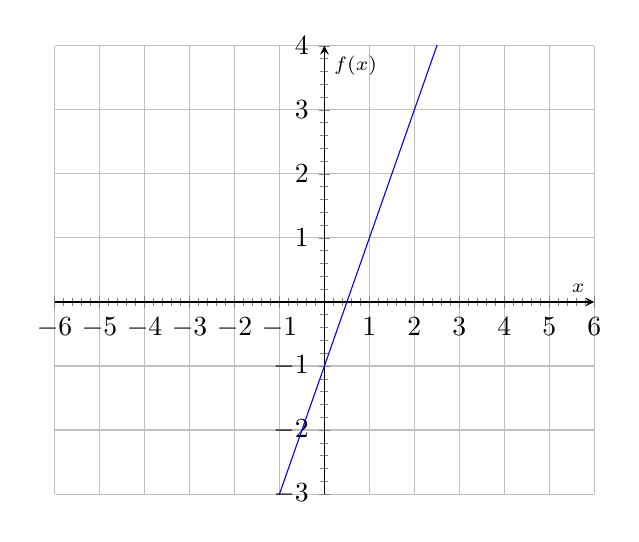
\begin{tikzpicture}[scale=1.0]
    \begin{axis}%
        [
            grid=major,
            xtick={-7,-6,...,7},
            minor x tick num=4, % 4 minor ticks => 5 subintervals
            xmin=-6,
            xmax=6,
            xlabel={\scriptsize $x$},
            axis x line=middle,
            ytick={-5,-4,...,5},
            minor y tick num=4,  % 4 minor ticks => 5 subintervals
            ymin=-3,
            ymax=4,
            ylabel={\scriptsize $f(x)$},
            axis y line=middle,
            no markers,
            samples=100,
            domain=-6:6,
        ]
        \addplot (x,{2*x-1});
    \end{axis}
\end{tikzpicture}

\break
\newpage
\subsection{Zusammenfassung aller Funtionstypen}

\begin{enumerate}
    \item Lineare Funktion: $f(x)=mx+n$ \begin{itemize}
              \item Definitionsbereich: $x\in\mathbb{R}$
              \item Wertebereich: $y\in\mathbb{R}$
              \item Nullstelle: $x_0=-\frac{n}{m}$
              \item streng monoton steigend
          \end{itemize}
    \item Quadratische Funktion: $f(x)=x^2+px+q$ \begin{itemize}
              \item Definitionsbereich: $x\in\mathbb{R}$
              \item Wertebereich: $x\in\mathbb{R},\geq-\frac{p^2}{4}+4$
              \item Nullstelle: $x_{1,2}=+\frac{p}{2} \pm \sqrt{\binom{p}{2}^2-q}$
              \item streng monoton steigend für $x \geq -\frac{p}{2}$
              \item streng monoton fallend für $x \leq -\frac{p}{2}$
          \end{itemize}
    \item Quadratische Funktion: $f(x)=ax^2+e$ \begin{itemize}
              \item Definitionsbereich: $x\in\mathbb{R}$
              \item Wertebereich: $y\in\mathbb{R},y\leq e$
              \item Nullstelle: $x_{1,2} = \pm \sqrt{-\frac{e}{a}}$
              \item streng monoton steigend für $x<0$
              \item streng monoton fallend für $x>0$
          \end{itemize}
    \item Wurzelfunktion: $f(x)=\sqrt{x}$\begin{itemize}
              \item Definitionsbereich: $x\in\mathbb{R},y\geq 0$
              \item Wertebereich: $y\in\mathbb{R},y\geq 0$
              \item Nullstelle: $x_0=0$
              \item streng monoton steigend
          \end{itemize}
    \item Potenzfunktion: $f(x)=x^n$\begin{itemize}
              \item Definitionsbereich: $x\in\mathbb{R},y\neq 0$
              \item Wertebereich: $y\in\mathbb{R},y\neq 0$
              \item Nullstelle: Nicht vorhanden
              \item streng monoton fallend für $x \neq 0$
          \end{itemize}
    \item Sinusfunktion: $f(x=sin(x))$\begin{itemize}
              \item Definitionsbereich: $x\in\mathbb{R}$
              \item Wertebereich: $y\in\mathbb{R},-1 \leq y \leq 1$
              \item Nullstelle: $x_k=k * \pi,k \in \mathbb{Z}$
              \item streng monoton steigend für $-\frac{\pi}{2}\leq x \leq \frac{\pi}{2}$
              \item streng monoton fallend für $\frac{\pi}{2}\leq x \leq \frac{3\pi}{2}$
          \end{itemize}
    \item Exponential-funktion: $f(x)=a*b^x$\begin{itemize}
              \item Definitionsbereich: $x\in\mathbb{R}$
              \item Wertebereich: $y\in\mathbb{R},y > 0$
              \item Nullstelle: Nicht vorhanden
              \item streng monoton fallend für
          \end{itemize}
    \item Logarithmus-funktion: $f(x)=log_b(x)$\begin{itemize}
              \item Definitionsbereich: $x\in\mathbb{R},x > 0$
              \item Wertebereich: $y\in\mathbb{R}$
              \item Nullstelle: $x_0=1$
              \item streng monoton steigend für
          \end{itemize}
\end{enumerate}


\break
\newpage
\subsection{Steigung}

Die Steigung ist das Verhältnis von $x$ zu $y$.\\
Am Beispiel von $y = -2x+5$ bei einem Schritt von $+1$ nach $x$ ändert sich $y$ um $-2$ daher ist die Steigung $\frac{-2}{1}$.


\hfill \break
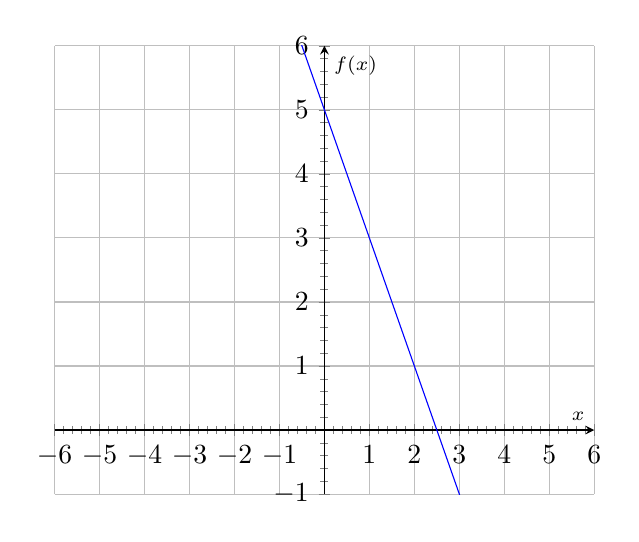
\begin{tikzpicture}[scale=1.0]
    \begin{axis}%
        [
            grid=major,
            xtick={-7,-6,...,7},
            minor x tick num=4, % 4 minor ticks => 5 subintervals
            xmin=-6,
            xmax=6,
            xlabel={\scriptsize $x$},
            axis x line=middle,
            ytick={-5,-4,...,6},
            minor y tick num=4,  % 4 minor ticks => 5 subintervals
            ymin=-1,
            ymax=6,
            ylabel={\scriptsize $f(x)$},
            axis y line=middle,
            no markers,
            samples=100,
            domain=-6:6,
        ]
        \addplot (x,{-2*x+5});
        \slopeTriangle{0.8}{0.1}{0.5}{1}{blue}; % USE OF MACRO.
    \end{axis}
\end{tikzpicture}
\break
\newpage
\subsection{Einteilung der Funktionen}

Funktionen werden in verschiedenen Arten unterschieden:\\
\begin{enumerate}
    \item Funktion 1.Grades (Lineare Funktion):\textcolor{red}{$f(x)=a+x^1+d$}
    \item Funktion 2.Grades (Quadratische Funktion):\textcolor{blue}{$f(x)=ax^2+bx^1+d$}
    \item Funktion 3.Grades (Kubische Funktion):\textcolor{violet}{$f(x)=ax^3+bx^2+cx^1+d$}
\end{enumerate}


\hfill \break
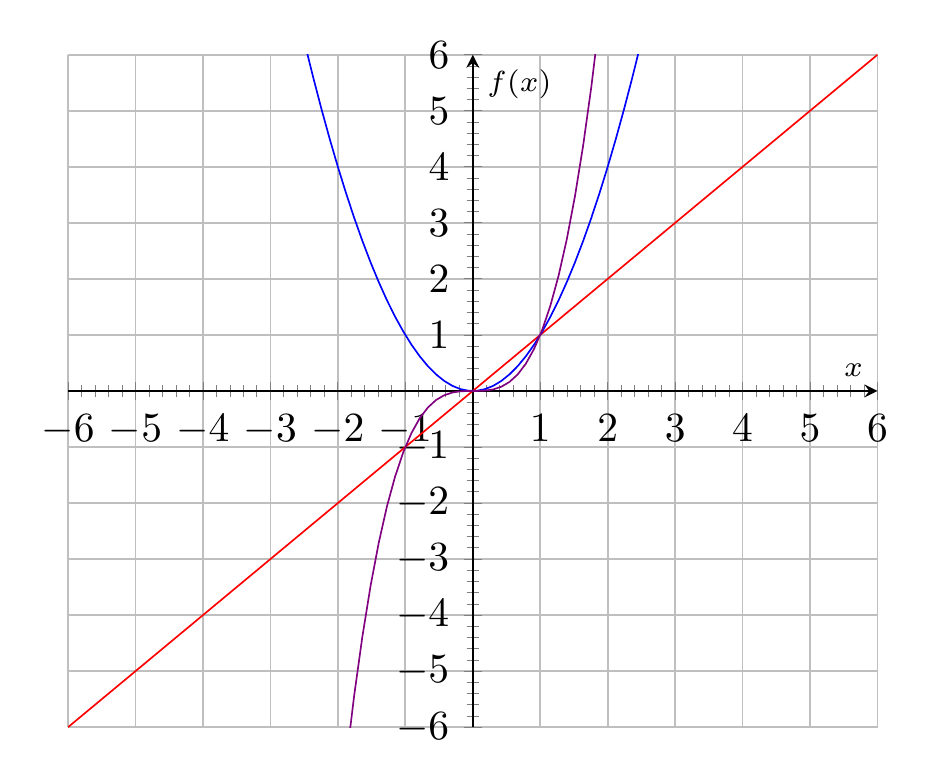
\begin{tikzpicture}[scale=1.5]
    \begin{axis}%
        [
            grid=major,
            xtick={-7,-6,...,7},
            minor x tick num=4, % 4 minor ticks => 5 subintervals
            xmin=-6,
            xmax=6,
            xlabel={\scriptsize $x$},
            axis x line=middle,
            ytick={-6,-5,...,7},
            minor y tick num=4,  % 4 minor ticks => 5 subintervals
            ymin=-6,
            ymax=6,
            ylabel={\scriptsize $f(x)$},
            axis y line=middle,
            no markers,
            samples=100,
            domain=-6:6,
        ]
        \addplot[red] (x,{x});
        \addplot[blue] (x,{x*x});
        \addplot[violet] (x,{x*x*x});
    \end{axis}
\end{tikzpicture}
\break
\newpage
\subsection{Lineare Funktionen}

Die Grundform einer jeden linearen Funktion ist $y=k*x+d$.
Wobei...

\begin{itemize}
    \item ... $y$ das das Resultat der Gleichung ist
    \item ... $k$ die Steigung der linearen Funktion ist
    \item ... $x$ die Variable ist
    \item ... $d$ der Abstand zur $x$ Achse ist
\end{itemize}

\hfill \break
Wenn das $k$ der Gleichung...
\begin{itemize}
    \item $>0$ ist wird die Gerade steigend z.B. \textcolor{red}{$y=3x+1$}
    \item $<0$ ist wird die Gerade fallend z.B. \textcolor{green}{$y=-3x+1$}
    \item $=0$ ist wird die Gerade waagrecht z.B. \textcolor{blue}{$y=1$}
\end{itemize}

\hfill \break
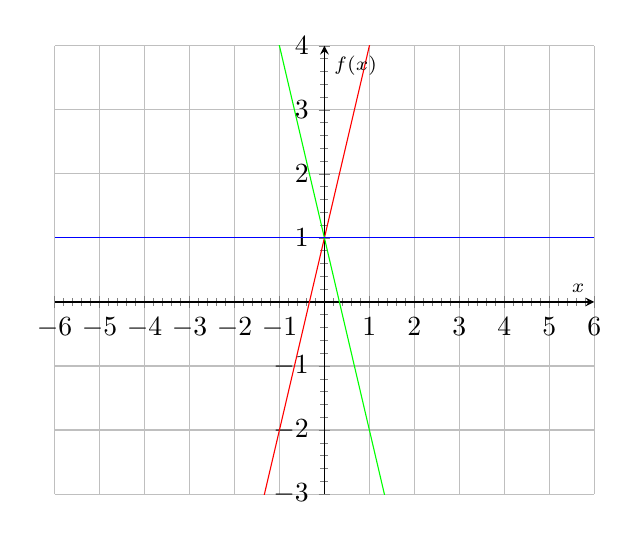
\begin{tikzpicture}[scale=1.0]
    \begin{axis}%
        [
            grid=major,
            xtick={-7,-6,...,7},
            minor x tick num=4, % 4 minor ticks => 5 subintervals
            xmin=-6,
            xmax=6,
            xlabel={\scriptsize $x$},
            axis x line=middle,
            ytick={-5,-4,...,5},
            minor y tick num=4,  % 4 minor ticks => 5 subintervals
            ymin=-3,
            ymax=4,
            ylabel={\scriptsize $f(x)$},
            axis y line=middle,
            no markers,
            samples=100,
            domain=-6:6,
        ]
        \addplot[red] (x,{3*x+1});
        \addplot[green] (x,{-3*x+1});
        \addplot[blue] (x,{1});
    \end{axis}
\end{tikzpicture}
\break
\newpage
\subsection{Lineare Funktionen mit 2 Variablen}

Jede lineare Gleichung lässt sich auf eine Faktorgleichung der Form $y=kx+d$ umformen.
$$ax+by = c$$
$$\downarrow$$
$$y=\frac{c-ax}{b}$$

\hfill \break
Example:\\
\fboxrule=0.8pt \fcolorbox{black}{lightgray}{%
    \begin{tabular}[t]{@{}l@{}}
        $x+y=5$ /-x \\
        $y=5-x$     \\
        $y=-x+5$    \\
        $y=-1x+5$   \\
    \end{tabular}}
\begin{itemize}
    \item $d=5$
    \item $k=-1$
\end{itemize}

\hfill \break
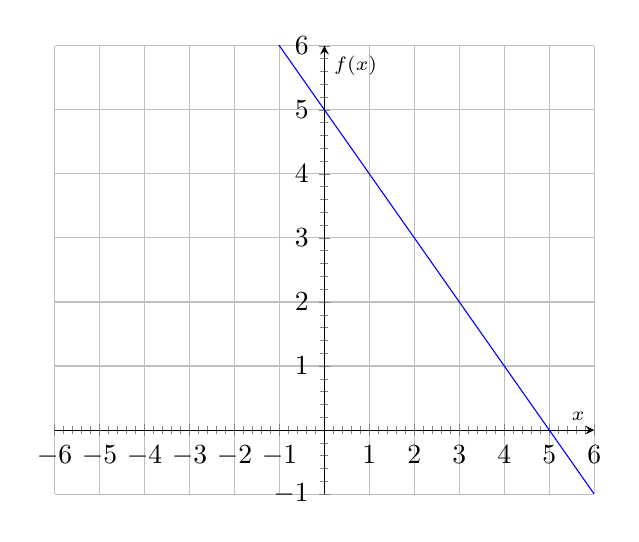
\begin{tikzpicture}[scale=1.0]
    \begin{axis}%
        [
            grid=major,
            xtick={-7,-6,...,7},
            minor x tick num=4, % 4 minor ticks => 5 subintervals
            xmin=-6,
            xmax=6,
            xlabel={\scriptsize $x$},
            axis x line=middle,
            ytick={-5,-4,...,6},
            minor y tick num=4,  % 4 minor ticks => 5 subintervals
            ymin=-1,
            ymax=6,
            ylabel={\scriptsize $f(x)$},
            axis y line=middle,
            no markers,
            samples=100,
            domain=-6:6,
        ]
        \addplot (x,{-1*x+5});
    \end{axis}
\end{tikzpicture}

\hfill \break
Lösungsverfahren:
\begin{itemize}
    \item Graphisch
    \item Rechnerisches Gleichsetzungsverfahren
    \item Rechnerisches Einsetzungsverfahren
    \item Rechnerisches Eliminationsverfahren
\end{itemize}

\break
\newpage
\subsubsection{Gleichsetzungsverfahren}

Beim Gleichsetzungsverfahren werden beide Terme Gleichgesetzt.

\hfill \break
Example:\\
\fboxrule=0.8pt \fcolorbox{black}{lightgray}{%
    \begin{tabular}[t]{@{}l@{}}
        (1):$y=x+1 $ / $y=2$   \\
        (2):$y=-2x+4 $ / $y=2$ \\
        \\
        \\
        $y_1 = y_2$            \\
        $x+1 = -2x+4$ /+2x     \\
        $3x+1 = 4$ /-1         \\
        $3x = 3$ / /3          \\
        $x = 1$                \\
    \end{tabular}}

$$L=\{1,2\}$$
\break
\subsubsection{Einsezuungsverfahren}

Beim Einsezuungsverfahren wird ein Term in den anderen eingesetzt.

\hfill \break
Example:\\
\fboxrule=0.8pt \fcolorbox{black}{lightgray}{%
    \begin{tabular}[t]{@{}l@{}}
        (1):$y=x+1$                                  \\
        (2):$+2x+y=4$ / $x+1$ wird in $y$ eingesetzt \\
        \\
        \\
        $+2x+x+1 = 4$                                \\
        $3x+1 = 4$ / -1                              \\
        $3x = 3$ / /3                                \\
        $x = 1$                                      \\
    \end{tabular}}

$$L=\{1,2\}$$
\break
\newpage
\subsubsection{Eliminationsverfahren}

Beim Eliminationsverfahren wird ein Teil des ersten Termes vom zweiten Term subtrahiert.

\hfill \break
Example:\\
\fboxrule=0.8pt \fcolorbox{black}{lightgray}{%
    \begin{tabular}[t]{@{}l@{}}
        (1):$y=x+1$ /$y$ wird elemeniert   \\
        (2):$y=-2x+4$ /$y$ wird elemeniert \\
        \\
        \\
        $0=x-(-2x)+1-4$                    \\
        $0=x+2x-3$                         \\
        $3=3x$ / /3                        \\
        $1=x$                              \\
    \end{tabular}}

$$L=\{1,2\}$$

\hfill \break
Um $x$ elemenieren zu können muss man zuerst bei beide Gleichungen die selbe Anzahl an $x$ erzeugen.

\hfill \break
Example:\\
\fboxrule=0.8pt \fcolorbox{black}{lightgray}{%
    \begin{tabular}[t]{@{}l@{}}
        (1):$4x + y = 16$          \\
        (2):$4x - 2y  = - 8 $ / /2 \\
        (2):$2x - y  = - 4$        \\
        \\
        \\
        $4x+y=16$                  \\
        $2x-y=-4$                  \\
        $6x=12$                    \\
        $x=2$                      \\
        \\
        \\
        In Ursprungsform Einsetzen \\
        $4*2+y=16$                 \\
        $8+y=16$ / -8              \\
        $y=8$                      \\
    \end{tabular}}

$$L=\{2,8\}$$
\newpage
\subsubsection{Sonderfälle}

\hfill \break
Example 1.Sonderfall:\\
\fboxrule=0.8pt \fcolorbox{black}{lightgray}{%
    \begin{tabular}[t]{@{}l@{}}
        (1):$3x+2y=4$ / *2 \\
        (2):$-6x-4y=-8$    \\
        (1):$6x+4y=8$      \\
        \\
        \\
        $0+0 = 0$          \\
        $0 = 0$            \\
    \end{tabular}}\\

\hfill \break
Example 2.Sonderfall:\\
\fboxrule=0.8pt \fcolorbox{black}{lightgray}{%
    \begin{tabular}[t]{@{}l@{}}
        (1):$3x+2y=4$ / *3 \\
        (2):$9x+6y=10$     \\
        (1):$9x+6y=12$     \\
        \\
        \\
        $0+0 = 2$          \\
        $0 = 2$ / $f.A$    \\
    \end{tabular}}\\
\break
\newpage
\subsection{Funktionsgleichung bestimmen}

Es gibt zwei Arten der Bestimmung der Funktionsgleichung:\\

\hfill \break
\fboxrule=0.8pt \fcolorbox{black}{lightgray}{%
    \begin{tabular}[t]{@{}l@{}}
        $A(1/8)$  \\
        $B(-4/3)$ \\
        \hline
        $y=kx+d$
    \end{tabular}}\\

\hfill \break
1.Graphisch:\\
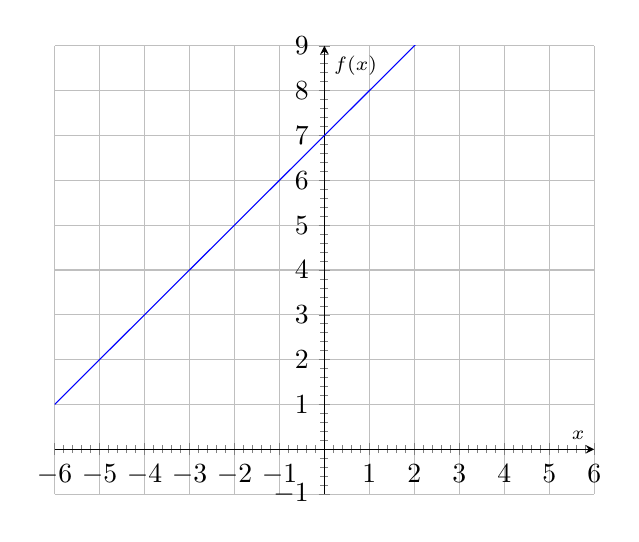
\begin{tikzpicture}[scale=1.0]
    \begin{axis}%
        [
            grid=major,
            xtick={-7,-6,...,7},
            minor x tick num=4, % 4 minor ticks => 5 subintervals
            xmin=-6,
            xmax=6,
            xlabel={\scriptsize $x$},
            axis x line=middle,
            ytick={-5,-4,...,9},
            minor y tick num=4,  % 4 minor ticks => 5 subintervals
            ymin=-1,
            ymax=9,
            ylabel={\scriptsize $f(x)$},
            axis y line=middle,
            no markers,
            samples=100,
            domain=-6:6,
        ]
        \addplot[blue] (x,{x+7});
    \end{axis}
\end{tikzpicture}

\hfill \break
\fboxrule=0.8pt \fcolorbox{black}{lightgray}{%
    \begin{tabular}[t]{@{}l@{}}
            $d=7$ \\
            $k=1$ \\
            \hline
            $y=kx+d$
        \end{tabular}}\\

\hfill \break
2.Rechnerisch:\\
\fboxrule=0.8pt \fcolorbox{black}{lightgray}{%
    \begin{tabular}[t]{@{}l@{}}
            (1):$8=1k+d$                                            \\
            (2):$\textcolor{blue}{3=-4k+d}$                         \\
            (1):$d=-k+8$                                            \\
            $3=-4k-k+8$ / ermittelt durch das Eliminationsverfahren \\
            $k=\textcolor{red}{1}$                                  \\
            \\
            $\textcolor{blue}{3=-4*\textcolor{red}{1}+d}$           \\
            $d=7$                                                   \\
        \end{tabular}}\\
\break
\newpage
\subsection{Kostenfunktion}

Die Grundform der Kostenfunktion ist $K(x)=k*x+F$.
Wobei...
\begin{itemize}
    \item ... $K(x)$ ist das Resultat der Gleichung ist also die Kosten.
    \item ... $k$ die Kosten pro Stück darstellt
    \item ... $x$ die Menge ist
    \item ... $F$ die Fixkosten darstellt
\end{itemize}

\hfill \break
Die Grundform der Erlösfunktion ist $E(x)=p*x$.
Wobei...
\begin{itemize}
    \item ... $E(x)$ ist das Resultat der Gleichung ist also der Erlös des Verkaufs
    \item ... $p$ der Verkaufspreis
    \item ... $x$ die Verkaufsmenge ist
\end{itemize}

\hfill \break
Die Grundform der Gewinnfunktion ist $G(x)=E(x)-K(x)$.
Wobei $G(x)$ der Gewinn ist.

\hfill \break
Example:\\
Die Fixkosten eines Betriebes betragen 140000€ pro Monat, die Produktionskosten 4€ pro Stück. Ein Stück wird zu 8€
verkauft.
Wie viel Stück müssen verkauft werden, damit ein Gewinn von mindestens 1000 000€ erzielt wird?:\\
\fboxrule=0.8pt \fcolorbox{black}{lightgray}{%
    \begin{tabular}[t]{@{}l@{}}
        $K(x)=4x+140000$             \\
        $E(x)=8x$                    \\
        $G(x)=E(x)-K(x)$             \\
        \hline
        $1000000=8x-(4x+140000)$     \\
        $1000000=8x-4x-140000$       \\
        $1000000=4x-140000$ /+140000 \\
        $1140000=4x$ / /4            \\
        $x=285000$                   \\
    \end{tabular}}
\break
\newpage
\subsection{Normale/Paralelle Lineare Funktionen}

Die zu einer Geraden normale Gerade erhält man durch den negativen Kehrwert: $K\bot = -\frac{1}{k}$

\hfill \break
Example normale Funktionenen:\\
\fboxrule=0.8pt \fcolorbox{black}{lightgray}{%
    \begin{tabular}[t]{@{}l@{}}
        $\textcolor{red}{y=\frac{3}{4}x}$      \\
        $\textcolor{green}{y_n=-\frac{4}{3}x}$ \\
    \end{tabular}}

\hfill \break
Example paralelle Funktionenen:\\
\fboxrule=0.8pt \fcolorbox{black}{lightgray}{%
    \begin{tabular}[t]{@{}l@{}}
        $\textcolor{blue}{y = 3x-1}$   \\
        $\textcolor{violet}{y = 3x+3}$ \\
    \end{tabular}}

\hfill \break
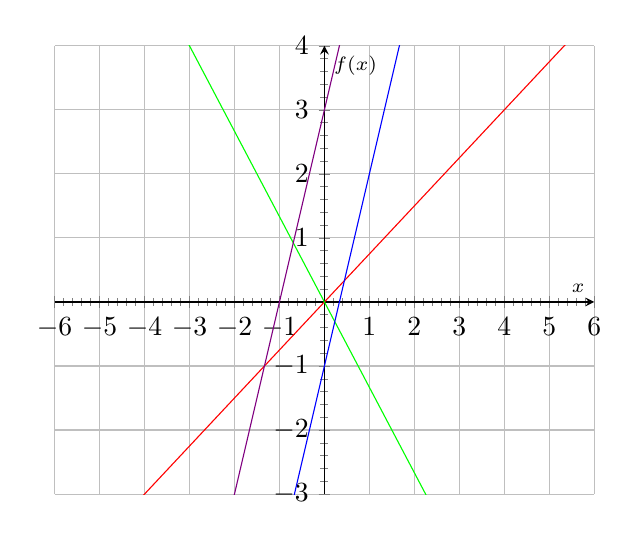
\begin{tikzpicture}[scale=1.0]
    \begin{axis}%
        [
            grid=major,
            xtick={-7,-6,...,7},
            minor x tick num=4, % 4 minor ticks => 5 subintervals
            xmin=-6,
            xmax=6,
            xlabel={\scriptsize $x$},
            axis x line=middle,
            ytick={-5,-4,...,5},
            minor y tick num=4,  % 4 minor ticks => 5 subintervals
            ymin=-3,
            ymax=4,
            ylabel={\scriptsize $f(x)$},
            axis y line=middle,
            no markers,
            samples=100,
            domain=-6:6,
        ]
        \addplot[red] (x,{(3/4)*x});
        \addplot[green] (x,{-(4/3)*x});
        \addplot[blue] (x,{3*x-1});
        \addplot[violet] (x,{3*x+3});
    \end{axis}
\end{tikzpicture}

\hfill \break
Example normale Funktionenen:\\
\fboxrule=0.8pt \fcolorbox{black}{lightgray}{%
    \begin{tabular}[t]{@{}l@{}}
        $y_1 = \frac{2}{3}x \bot y_1=-\frac{3}{2}x$ \\
        \\
        $y_2 = 2x \bot y_2=+\frac{1}{2}x$           \\
        \\
        $y_3 = -\frac{1}{3}x+1 \bot y_3=3x+1$       \\
    \end{tabular}}

\hfill \break
Example paralelle Funktionenen:\\
\fboxrule=0.8pt \fcolorbox{black}{lightgray}{%
    \begin{tabular}[t]{@{}l@{}}
        $y_1 = 3x-1 \| y_1 = 3x+1 $            \\
        \\
        $y_2 = 10x+101 \| y_2 = 10x-8 $        \\
        \\
        $y_3 = 5x+83 \| y_3 = 5x+\frac{1}{2} $ \\
    \end{tabular}}
\break
\newpage
\subsection{Funktionswerte}

\hfill \break
\subsubsection{steigen und sinken}

Es gibt verschieden Arten von Funktionen:\\
\begin{itemize}
    \item \textcolor{red}{Streng monoton steigend $f'(x)>0$}
    \item \textcolor{violet}{Konstant $f'(x)=0$}
    \item \textcolor{blue}{Streng monoton fallend $f'(x)<0$ }
\end{itemize}

\hfill \break

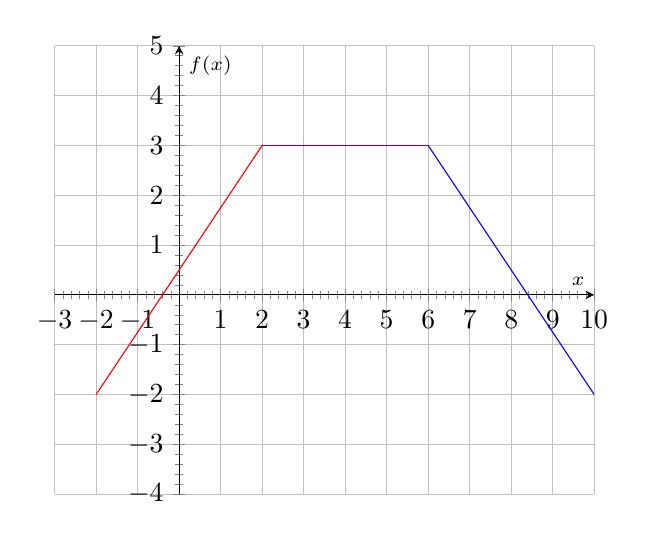
\begin{tikzpicture}[scale=1.0]
    \begin{axis}%
        [
            grid=major,
            xtick={-7,-6,...,11},
            minor x tick num=4, % 4 minor ticks => 5 subintervals
            xmin=-3,
            xmax=10,
            xlabel={\scriptsize $x$},
            axis x line=middle,
            ytick={-6,-5,...,6},
            minor y tick num=4,  % 4 minor ticks => 5 subintervals
            ymin=-4,
            ymax=5,
            ylabel={\scriptsize $f(x)$},
            axis y line=middle,
            no markers,
            samples=100,
            domain=-6:6,
        ]
        \draw[red] (-2,-2) -- (2,3);
        \draw[violet] (2,3) -- (6,3);
        \draw[blue] (6,3) -- (10,-2);
    \end{axis}
\end{tikzpicture}
\hfill \break
\newpage
\subsubsection{globale und lokale Extreme}

\begin{itemize}
    \item \textcolor{red}{${a,b}$ sind Randextreme}
    \item \textcolor{violet}{$x_1,x_2$ sind lokale Extreme}
\end{itemize}

\hfill \break
\begin{itemize}
    \item Globale Extrmes sind Extreme bezüglich des Gesammten Definitionsbereich.
    \item Lobale Extrmes sind Extreme bezüglich eines klienen Bereiches.
    \item Extremstellen haben wagrechte Tangenten mit der Steigung $0$
\end{itemize}

\hfill \break
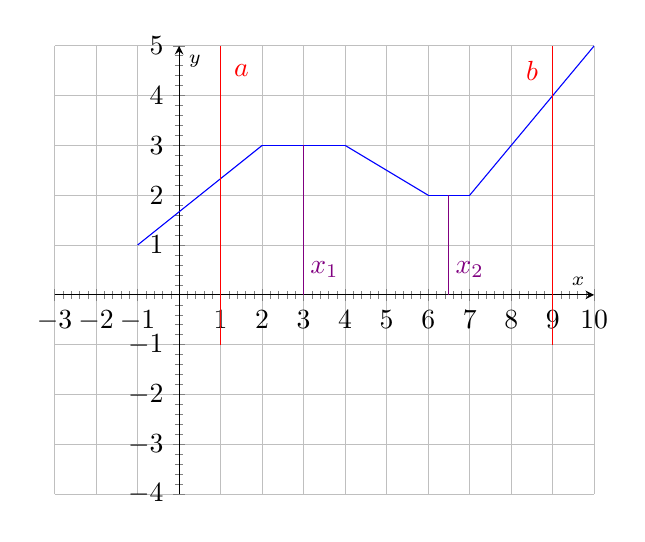
\begin{tikzpicture}[scale=1.0]
    \begin{axis}%
        [
            grid=major,
            xtick={-7,-6,...,11},
            minor x tick num=4, % 4 minor ticks => 5 subintervals
            xmin=-3,
            xmax=10,
            xlabel={\scriptsize $x$},
            axis x line=middle,
            ytick={-6,-5,...,6},
            minor y tick num=4,  % 4 minor ticks => 5 subintervals
            ymin=-4,
            ymax=5,
            ylabel={\scriptsize $y$},
            axis y line=middle,
            no markers,
            samples=100,
            domain=-6:6,
        ]
        \draw[blue] (-1,1) -- (2,3);
        \draw[blue] (2,3) -- (4,3);
        \draw[blue] (4,3) -- (6,2);
        \draw[blue] (6,2) -- (7,2);
        \draw[blue] (7,2) -- (10,5);
        \draw[red] (1,-1) -- (1,5);
        \draw[red] (9,-1) -- (9,5);
        \node[red] at (1.5,4.5) {$a$};
        \node[red] at (8.5,4.5) {$b$};

        \draw[violet] (3,0) -- (3,3);
        \draw[violet] (6.5,0) -- (6.5,2);
        \node[violet] at (3.5,0.5) {$x_1$};
        \node[violet] at (7,0.5) {$x_2$};
    \end{axis}
\end{tikzpicture}
\break
\newpage
\subsection{Quadratische Funktionen}

\begin{itemize}
    \item Die Grundform ist $y=a(x+b)^2+c$
    \item Faktorisierte Form ist $f(x)=a(x+x_1)*(x-x_2)$
    \item Scheitelpunktform oder Scheitelform ist $f(x)=a(x-d)^2+e$ mit Scheitel $S(d|e)$
\end{itemize}

\hfill \break
Veränderung der Normparabel:
\begin{itemize}
    \item Normparabel: \textcolor{black}{$x^2$}
    \item ist \textcolor{red}{$a<0$} wird die Funktion an der x Achse gespiegelt.
    \item ist \textcolor{blue}{$0<a<1$} wird die Funktion breiter bezihungsweise gestaucht.
    \item ist \textcolor{violet}{$a>1$} wird die Funktion steiler.
    \item ist \textcolor{cyan}{$x>0$} wird die Funktion nach oben verschoben.
    \item ist \textcolor{orange}{$x<0$} wird die Funktion nach oben verschoben.
    \item ist \textcolor{green}{$y<0$} wird die Funktion nach rechts verschoben.
    \item ist \textcolor{brown}{$y>0$} wird die Funktion nach links verschoben.
\end{itemize}

\hfill \break
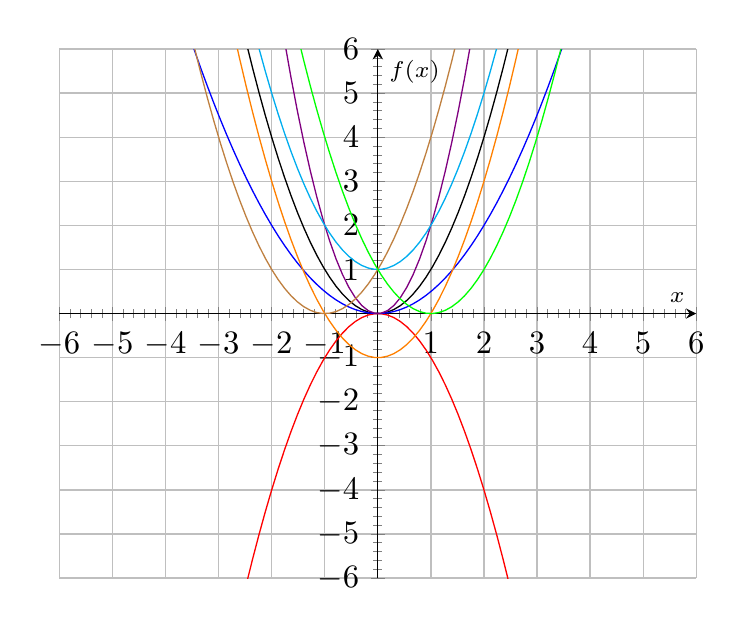
\begin{tikzpicture}[scale=1.18]
    \begin{axis}%
        [
            grid=major,
            xtick={-7,-6,...,7},
            minor x tick num=4, % 4 minor ticks => 5 subintervals
            xmin=-6,
            xmax=6,
            xlabel={\scriptsize $x$},
            axis x line=middle,
            ytick={-7,-6,...,7},
            minor y tick num=4,  % 4 minor ticks => 5 subintervals
            ymin=-6,
            ymax=6,
            ylabel={\scriptsize $f(x)$},
            axis y line=middle,
            no markers,
            samples=100,
            domain=-6:6,
        ]
        \addplot[black] (x,{x^2});
        \addplot[red] (x,{-1*x^2});
        \addplot[blue] (x,{0.5*x^2});
        \addplot[violet] (x,{2*x^2});
        \addplot[cyan] (x,{x^2+1});
        \addplot[orange] (x,{x^2-1});
        \addplot[brown] (x,{(x+1)^2});
        \addplot[green] (x,{(x-1)^2});
    \end{axis}
\end{tikzpicture}
\break
\newpage
\subsection{Nullstellenberechnung}

Nullstellen sind Stellen an denen eine Funktion die $x$ Achse schneidet. Dort ist der Funktionswert $0$.
Diese könne einfach mit der ABC-Formel gelöst werden in dem dei Faktoren eisetzt.\\

Example:\\
\fboxrule=0.8pt \fcolorbox{black}{lightgray}{%
    \begin{tabular}[t]{@{}l@{}}
        $f(x)=0$   \\
        $-x^2+4=0$ \\
        $x^2=4$    \\
        $x=\pm 2$  \\
    \end{tabular}}\\

Example:\\
\fboxrule=0.8pt \fcolorbox{black}{lightgray}{%
    \begin{tabular}[t]{@{}l@{}}
        $3x^2+6x=0$   \\
        $3x(x-2)$     \\
        $x=\pm 2$     \\
        $x=0$         \\
        $x=2$         \\
        $N_1 = (0,0)$ \\
        $N_2 = (2,0)$ \\
    \end{tabular}}\\

Example:\\
\fboxrule=0.8pt \fcolorbox{black}{lightgray}{%
    \begin{tabular}[t]{@{}l@{}}
        $f(x)=-x^2+7x=0$                               \\
        $\textcolor{red}{x}\textcolor{blue}{(-x+7)}=0$ \\
        $x_1= \textcolor{red}{0}$                      \\
        $x_2=\textcolor{blue}{7}$                      \\
    \end{tabular}}\\

Example:\\
\fboxrule=0.8pt \fcolorbox{black}{lightgray}{%
    \begin{tabular}[t]{@{}l@{}}
        $f(x)=x^2-4x+3=0$                                 \\
        $x^2-4x\textcolor{red}{+4}=-3\textcolor{red}{+4}$ \\
        $(x\textcolor{red}{-2})^2 = 1$                    \\
        $x-2= \pm \sqrt{1}$                               \\
        $x = 2 \pm 1$                                     \\
        $x_1 = 3$                                         \\
        $x_2 = 1$                                         \\
    \end{tabular}}\\

Rechnungsweg im Taschenrechner $TI-82STATS$:\\
\begin{itemize}
    \item $2nd$ calc zerro
    \item Cursor 1 neben die nullstellen links plazieren 
    \item Cursor 2 neben die nullstellen rechts plazieren
\end{itemize}
\break
\newpage
\subsection{Funktionen Aufstellen}

2.
Die nebenstehende Kurve veranschaulicht die Wurfparabel eines vom Punkt A
rückgespielten Tennisballs. Der Abschusspunkt liegt 6m vor dem Netz in Höhe
von 0,60m. Der Ball überfliegt das Netz in einer Höhe von 1,20m (B) und trifft
6,00m hinter dem Netz den Boden (C).\\

\begin{itemize}
    \item (a) Man berechne die Funktionsgleichung der Wurfparabel.
    \item (b) Welche Höhe erreicht der Ball 2m nachdem er das Netz passiert hat.
    \item (c) Wo hat der Ball eine Höhe von 80cm?
\end{itemize}

\hfill \break


Angegebene Punkte:
\begin{itemize}
    \item $A = (-6|0.6)$
    \item $A = (0|1.2)$
    \item $A = (0|0)$
\end{itemize}

\hfill \break

Eingesetzt in die Glichung $f(x)=a*x^2+b*x+c$:
\begin{enumerate}
    \item $0.6 = 36a-6b+c$
    \item $1.2 = 0a+0b+c$
    \item $0 = 36a+6b+c$
\end{enumerate}

\hfill \break

A:
$\left(\begin{array}{ccccc}
            36 & -6 & 1 & 0.6 \\
            0  & 0  & 1 & 1.2 \\
            36 & 6  & 1 & 0   \\
        \end{array}\right)$\\

\hfill \break

Ergebnis der Matrix Rechnung:
\begin{itemize}
    \item $a = -0.025$
    \item $b = -0.05$
    \item $c = 1.2$
\end{itemize}

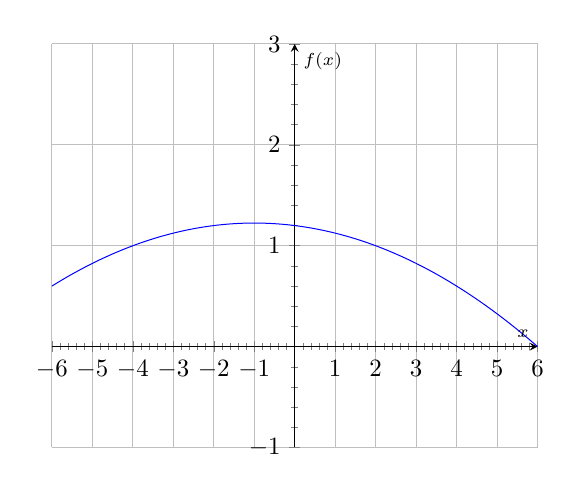
\begin{tikzpicture}[scale=0.9]
    \begin{axis}%
        [
            grid=major,
            xtick={-7,-6,...,7},
            minor x tick num=4, % 4 minor ticks => 5 subintervals
            xmin=-6,
            xmax=6,
            xlabel={\scriptsize $x$},
            axis x line=middle,
            ytick={-5,-4,...,3},
            minor y tick num=4,  % 4 minor ticks => 5 subintervals
            ymin=-1,
            ymax=3,
            ylabel={\scriptsize $f(x)$},
            axis y line=middle,
            no markers,
            samples=100,
            domain=-6:6,
        ]
        \addplot (x,{-0.025*x^2-0.05*x+1.2});
    \end{axis}
\end{tikzpicture}


\subsubsection{Lösung der Aufgabe A}
Die Funktionsgleichung wurden ermittelt in dem die Ergebnisse der Matrix in die Gleichung $f(x)=a*x^2+b*x+c$ Eingesetzt wurden.\\
Die Funktionsgleichung Lauted: $f(x)=-0.025x^2-0.05x+1.2$
\subsubsection{Lösung der Aufgabe B}
Bei dieser Aufgabe muss man den gewünschten Wert (in diesem Fall $2$) in die Funktionsgleichung die bei Beispiel $A$ errechnet wurde einsetzten.
Das Ergebnis lauted $1$
\subsubsection{Lösung der Aufgabe C}
Bei dieser Aufgabe werden die 80cm in Meter umgerechnet und als Ergebnis der Gleichung angegeben so, das $0.8 = -0.025x^2-0.05x+1.2$ entseht.
Danach muss die Gleichung durch eine Division durch $0.8$ noch auf die Form "0 = " gebracht werdendamit Man dei ABC-Formel anwenden kann.\\
die Ergebnisse lauten:
\begin{itemize}
    \item $x_1 = 3.12$
    \item $x_2 = 5.12$
\end{itemize}
\break
\newpage
\subsection{Exponentialfunktionen}


allgemeine Form: $y=a^x$
\begin{itemize}
    \item wenn $a>1$: Wachstum der Funktion
    \item wenn $0<a<1$: Zerfall der Funktion
\end{itemize}

\hfill \break
Eigenschaften:
\begin{itemize}
    \item alle Funktionen vom Typ $y=a^x$ haben den Punkt $P(0|1)$ gemein.
    \item alle Funktionen vom Typ $y=a^x$ gehen durch den Punkt $P(1|a)$, da $y=a^1 = a$.
    \item $y=a^x$ ist zu $y=a^{-x}$ symetrisch bezüglich der y Achse.
    \item die Funktion $y=a^x$ kann nie negativ werden also hat sie keine Nullstellen.
    \item Die x Achse ist eine Asymptote da die Funktion 0 niemals berührt.
\end{itemize}

\hfill \break
Die Wertetabellen und Grafik für \textcolor{red}{$y=2^x$} und \textcolor{blue}{$y=2^{-x}$}:\\

\hfill \break
\fboxrule=0.8pt \fcolorbox{lightgray}{lightgray}{%
    \begin{tabular}{c|c||c|c}
        \textcolor{red}{$x$} & $y$  & \textcolor{blue}{$x$} & $y$  \\
        \hline
        -2                   & 0.25 & -2                   & 4    \\
        -1                   & 0.5  & -1                   & 2    \\
        0                    & 1    & 0                    & 1    \\
        1                    & 2    & 1                    & 0.5  \\
        2                    & 4    & 2                    & 0.25 \\
    \end{tabular}}

\hfill \break
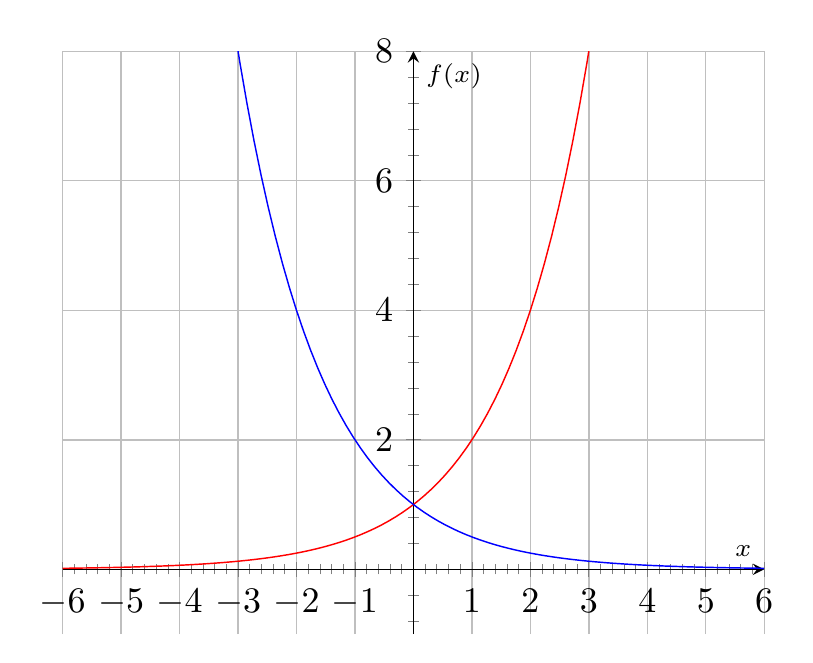
\begin{tikzpicture}[scale=1.3]
    \begin{axis}%
        [
            grid=major,
            xtick={-7,-6,...,7},
            minor x tick num=4, % 4 minor ticks => 5 subintervals
            xmin=-6,
            xmax=6,
            xlabel={\scriptsize $x$},
            axis x line=middle,
            ytick={-1,-5,...,7},
            minor y tick num=4,  % 4 minor ticks => 5 subintervals
            ymin=-1,
            ymax=8,
            ylabel={\scriptsize $f(x)$},
            axis y line=middle,
            no markers,
            samples=100,
            domain=-6:6,
        ]
        \addplot[red] (x,{2^x});
        \addplot[blue] (x,{2^-x});
    \end{axis}
\end{tikzpicture}
\break
\newpage
\subsection{Potenzfunktionen}

$y=a*x^n$ mit $a=1$


\hfill \break
\textcolor{red}{n positiv und gerade}
\begin{itemize}
    \item Definitionsmenge: $O = \mathbb{R}$
    \item Wertemenge: $W = \mathbb{R}_0^{+}$
    \item streng monoton fallend in: $\mathbb{R}_0^{-}$
    \item streng monoton steigend in: $\mathbb{R}_0^{+}$
    \item Alle Grapen gehen durch folgende Punkte: $P(-1|1),P(0|0),P(1|1)$
\end{itemize}

\hfill \break
\textcolor{green}{n positiv und ungerade}
\begin{itemize}
    \item Definitionsmenge: $O = \mathbb{R}$
    \item Wertemenge: $W = \mathbb{R}$
    \item streng monoton fallend in: --
    \item streng monoton steigend in: $\mathbb{R}$
    \item Alle Grapen gehen durch folgende Punkte: $P(-1|-1),P(0|0),P(1|1)$
\end{itemize}

\hfill \break
\textcolor{blue}{n negativ und gerade}
\begin{itemize}
    \item Definitionsmenge: $O = \mathbb{R}$ ohne $\{0\}$
    \item Wertemenge: $W = \mathbb{R}^{+}$
    \item streng monoton fallend in: $\mathbb{R}^{+}$
    \item streng monoton steigend in: $\mathbb{R}^{-}$
    \item Alle Grapen gehen durch folgende Punkte: $P(-1|1),P(1|1)$
    \item Asymptote: x und y Achsen $x=0$ $y=0$
\end{itemize}

\newpage
\textcolor{violet}{n negativ und gerade}
\begin{itemize}
    \item Definitionsmenge: $O = \mathbb{R}$ ohne $\{0\}$
    \item Wertemenge: $W = \mathbb{R}$ ohne $\{0\}$
    \item streng monoton fallend in: $\mathbb{R}$ ohne $\{0\}$
    \item streng monoton steigend in: --
    \item Alle Grapen gehen durch folgende Punkte: $P(-1|-1),P(1|1)$
    \item Asymptote: x und y Achsen $x=0$ $y=0$
\end{itemize}

\hfill \break
Graptische darstellung:
\hfill \break
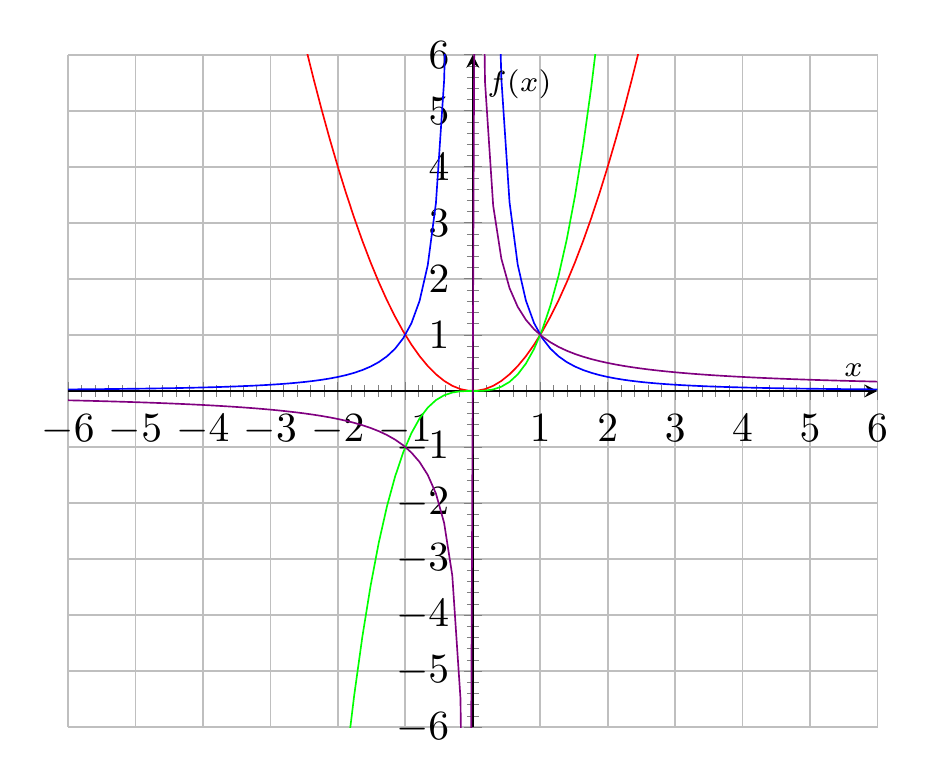
\begin{tikzpicture}[scale=1.5]
    \begin{axis}%
        [
            grid=major,
            xtick={-7,-6,...,7},
            minor x tick num=4, % 4 minor ticks => 5 subintervals
            xmin=-6,
            xmax=6,
            xlabel={\scriptsize $x$},
            axis x line=middle,
            ytick={-7,-6,...,7},
            minor y tick num=4,  % 4 minor ticks => 5 subintervals
            ymin=-6,
            ymax=6,
            ylabel={\scriptsize $f(x)$},
            axis y line=middle,
            no markers,
            samples=100,
            domain=-6:6,
        ]
        \addplot[red] (x,{1*x^2});
        \addplot[green] (x,{1*x^3});
        \addplot[blue] (x,{1*x^(-2)});
        \addplot[violet] (x,{1*x^(-1)});
    \end{axis}
\end{tikzpicture}
\break
\newpage
\subsection{Umkehr-Funktionen}

\hfill \break
\begin{itemize}
    \item Grapisch wird die Umkehrfunktionen durch das Spiegeln an der 1.Mediane ermittelt
    \item Rechnerisch wird die Umkehrfunktionen durch das Vertauschen von x und y ermittelt. zb.
          $y=10^x \rightarrow x=10^y \rightarrow y=Lg(x)$
\end{itemize}

\hfill \break
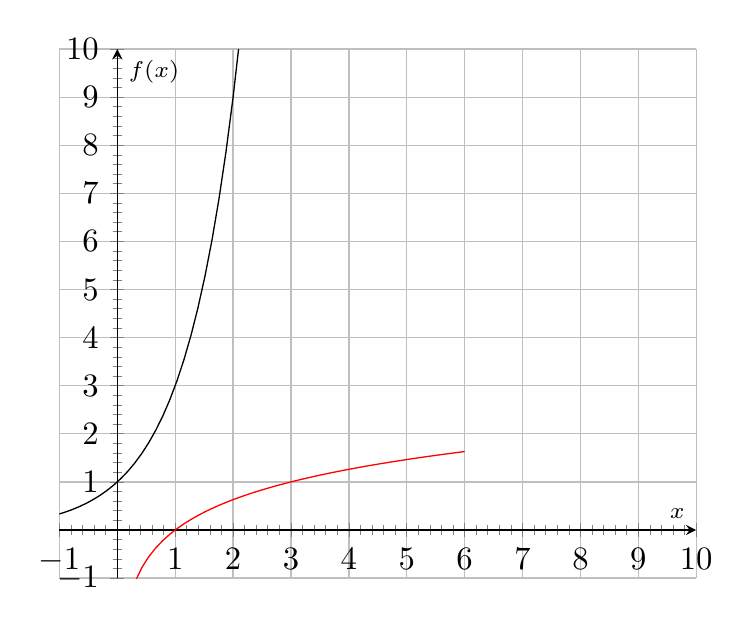
\begin{tikzpicture}[scale=1.18]
    \begin{axis}%
        [
            grid=major,
            xtick={-1,0,...,10},
            minor x tick num=4, % 4 minor ticks => 5 subintervals
            xmin=-1,
            xmax=10,
            xlabel={\scriptsize $x$},
            axis x line=middle,
            ytick={-1,0,...,10},
            minor y tick num=4,  % 4 minor ticks => 5 subintervals
            ymin=-1,
            ymax=10,
            ylabel={\scriptsize $f(x)$},
            axis y line=middle,
            no markers,
            samples=100,
            domain=-6:6
        ]
        \addplot[black] (x,{3^x});
        \addplot[red] (x,{ln(x)/ln(3)}); 
    \end{axis}
\end{tikzpicture}

\subsubsection{Graphen schneiden mit TR}

\hfill \break
Example:\\
\fboxrule=0.8pt \fcolorbox{black}{lightgray}{%
    \begin{tabular}[t]{@{}l@{}}
        $y = -x^3+8x-3$    \\
        $y = x^2-6x+9$     \\
        \\
        2nd calc intersect \\
        \\
        $S(1\vert4)$       \\
        $S(6\vert 9)$      \\
    \end{tabular}}\\

\break
\newpage
\section{Wachstum und Zerfall}


\hfill \break
Algemeines:
$$f(x) = c*a^x$$
$$\textcolor{red}{N(t)} = \textcolor{blue}{N_0}*\textcolor{green}{a}^t$$

\begin{itemize}
    \item \textcolor{red}{$N(t)$}: Die Menge die zum Zeitpunkt t (noch) vorhanden ist.
    \item \textcolor{blue}{$N_0$}: Anfangsmenge oder Startwert.
    \item \textcolor{green}{$a$}: Wachstumes-Zerfallsfaktor.
    \item bei $a>1$ ist es ein Zuwachs
    \item bei $0<a<1$ ist es ein Verfall
\end{itemize}


\hfill \break
Umrechnung zwischen Funktionstypen:
$$N(t) = \textcolor{blue}{2}*\textcolor{red}{1.03}^t  \longrightarrow  N(t) = \textcolor{blue}{16}*\textcolor{red}{e^\lambda}^t$$

$$\fboxrule=0.8pt \fcolorbox{black}{lightgray}{%
        \begin{tabular}[t]{@{}l@{}}
            $1.03 = e^\lambda$ | /Ln      \\
            $Ln(1.03) = \lambda * L_e(e)$ \\
            $\lambda = 0.02855...$        \\
            $N(t) = 2*e^0.02855...$       \\
        \end{tabular}}$$


\hfill \break
Thermologie:
\begin{itemize}
    \item Halbwertszeit: Ist jene Zeit t, die vergehen muss bis nur noch die Hälfte des Anfangswetes vorhanden ist.
    \item Verdopplungszeit: Ist jene Zeit t, die vergehen muss bis das Doppelte des Anfangswetes vorhanden ist.
\end{itemize}

\break
\subsection{Modelle}

\hfill \break
Lineares Modell:\\
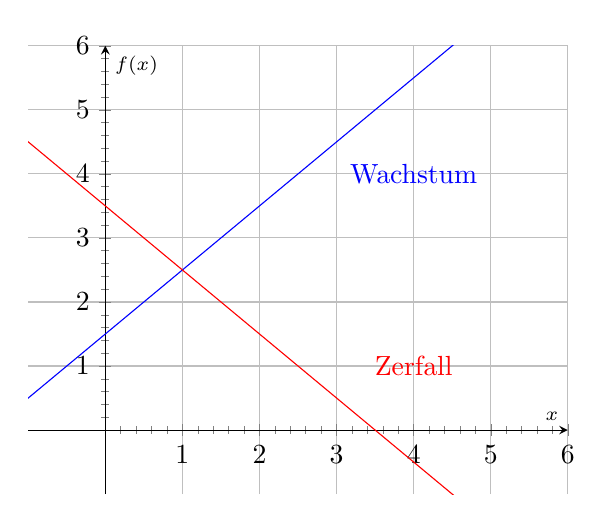
\begin{tikzpicture}[scale=1.0]
    \begin{axis}%
        [
            grid=major,
            xtick={0,1,...,7},
            minor x tick num=4, % 4 minor ticks => 5 subintervals
            xmin=-1,
            xmax=6,
            xlabel={\scriptsize $x$},
            axis x line=middle,
            ytick={0,1,...,7},
            minor y tick num=4,  % 4 minor ticks => 5 subintervals
            ymin=-1,
            ymax=6,
            ylabel={\scriptsize $f(x)$},
            axis y line=middle,
            no markers,
            samples=100,
            domain=-6:6,
        ]
        \addplot[blue] (x,{x+1.5});
        \addplot[red] (x,{-x+3.5});
        \node[color=blue] at (4,4) {Wachstum};
        \node[color=red] at (4,1) {Zerfall};
    \end{axis}
\end{tikzpicture}

\hfill \break
Exponentielles Modell:\\
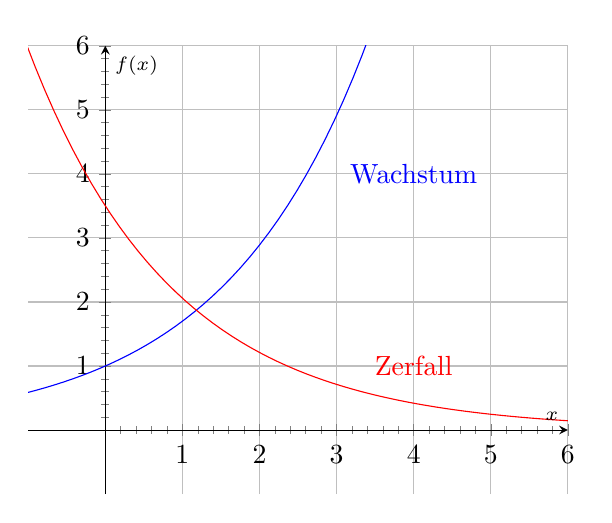
\begin{tikzpicture}[scale=1.0]
    \begin{axis}%
        [
            grid=major,
            xtick={0,1,...,7},
            minor x tick num=4, % 4 minor ticks => 5 subintervals
            xmin=-1,
            xmax=6,
            xlabel={\scriptsize $x$},
            axis x line=middle,
            ytick={0,1,...,7},
            minor y tick num=4,  % 4 minor ticks => 5 subintervals
            ymin=-1,
            ymax=6,
            ylabel={\scriptsize $f(x)$},
            axis y line=middle,
            no markers,
            samples=100,
            domain=-6:6,
        ]
        \addplot[blue] (x,{1.7^x});
        \addplot[red] (x,{3.5*(1.7^-x)});
        \node[color=blue] at (4,4) {Wachstum};
        \node[color=red] at (4,1) {Zerfall};
    \end{axis}
\end{tikzpicture}

\hfill \break
Beschränktes Wachstum:\\
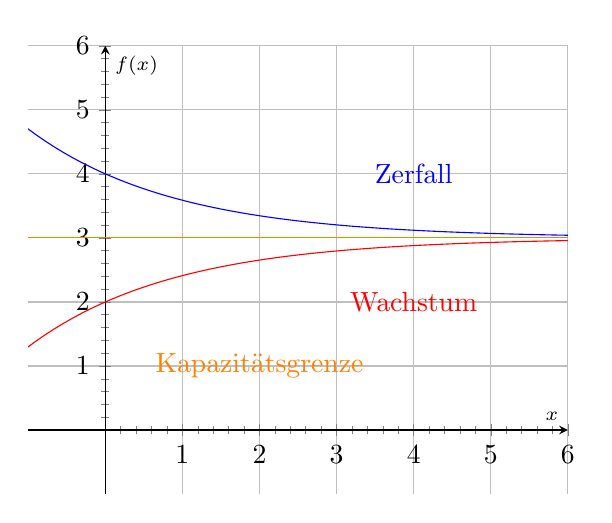
\begin{tikzpicture}[scale=1.0]
    \begin{axis}%
        [
            grid=major,
            xtick={0,1,...,7},
            minor x tick num=4, % 4 minor ticks => 5 subintervals
            xmin=-1,
            xmax=6,
            xlabel={\scriptsize $x$},
            axis x line=middle,
            ytick={0,1,...,7},
            minor y tick num=4,  % 4 minor ticks => 5 subintervals
            ymin=-1,
            ymax=6,
            ylabel={\scriptsize $f(x)$},
            axis y line=middle,
            no markers,
            samples=100,
            domain=-6:6,
        ]
        \addplot[blue] (x,{(1.7^-x)+3});
        \addplot[red] (x,{(-1.7^-x)+3});
        \node[color=blue] at (4,4) {Zerfall};
        \node[color=red] at (4,2) {Wachstum};
        \addplot[orange] (x,{3});
        \node[color=orange] at (2,1) {Kapazitätsgrenze};
    \end{axis}
\end{tikzpicture}

\hfill \break
Logisches Wachstum:\\
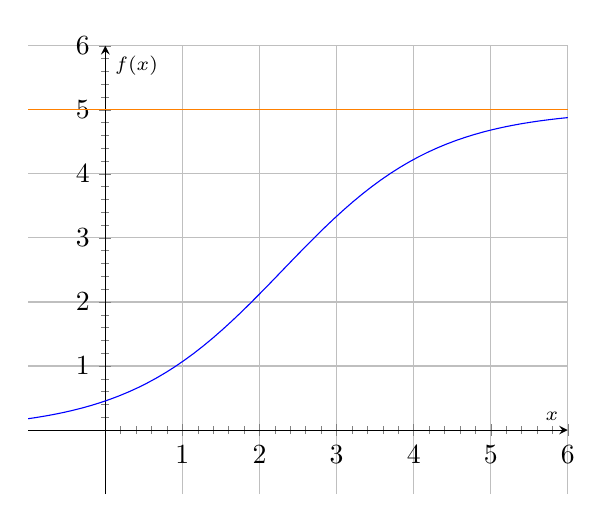
\begin{tikzpicture}[scale=1.0]
    \begin{axis}%
        [
            grid=major,
            xtick={0,1,...,7},
            minor x tick num=4, % 4 minor ticks => 5 subintervals
            xmin=-1,
            xmax=6,
            xlabel={\scriptsize $x$},
            axis x line=middle,
            ytick={0,1,...,7},
            minor y tick num=4,  % 4 minor ticks => 5 subintervals
            ymin=-1,
            ymax=6,
            ylabel={\scriptsize $f(x)$},
            axis y line=middle,
            no markers,
            samples=100,
            domain=-6:6,
        ]
        \addplot[orange] (x,{5});
        \addplot[blue] (x,{5/(1+10*e^-x)});
    \end{axis}
\end{tikzpicture}
\break
\newpage
\subsection{Lineares Modell}

\subsubsection{Wachstum}
\hfill \break
Es Ligen 25€ am Spaarbuch. Jede Woche werdern 5€ angespaart.
\hfill \break
$K(t)=\textcolor{red}{5}t+\textcolor{blue}{25}$

\begin{itemize}
    \item \textcolor{red}{5}: Zuanhme pro Woche (Konstant)
    \item \textcolor{blue}{25}: Startwert
\end{itemize}

\hfill \break
Darstellung:\\
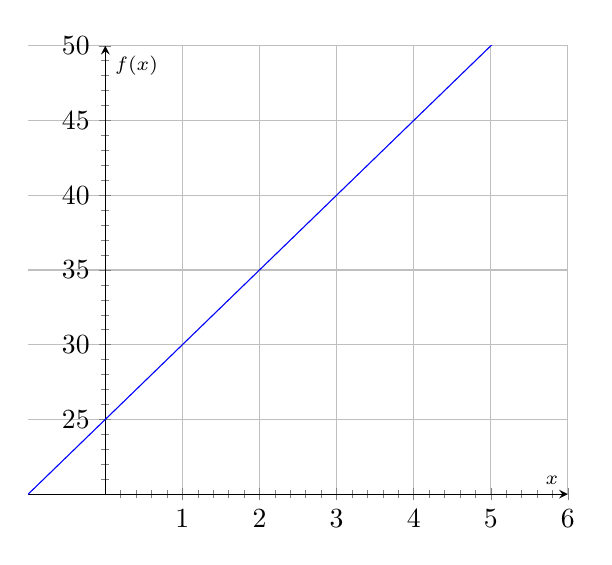
\begin{tikzpicture}[scale=1.0]
    \begin{axis}%
        [
            grid=major,
            xtick={0,1,...,7},
            minor x tick num=4, % 4 minor ticks => 5 subintervals
            xmin=-1,
            xmax=6,
            xlabel={\scriptsize $x$},
            axis x line=middle,
            ytick={20,25,...,50},
            minor y tick num=4,  % 4 minor ticks => 5 subintervals
            ymin=20,
            ymax=50,
            ylabel={\scriptsize $f(x)$},
            axis y line=middle,
            no markers,
            samples=100,
            domain=-6:6,
        ]
        \addplot[blue] (x,{5*x+25});
    \end{axis}
\end{tikzpicture}

\newpage
\subsubsection{Zerfall}

\hfill \break
Es Ligen 90€ auf einem Spaarbuch. Jede Woche werdern 5€ angehoben.
\hfill \break
$K(t)=\textcolor{red}{-5}t+\textcolor{blue}{90}$

\begin{itemize}
    \item \textcolor{red}{5}: Abnahme pro Woche (Konstant)
    \item \textcolor{blue}{25}: Startwert
\end{itemize}

\hfill \break
Darstellung:\\
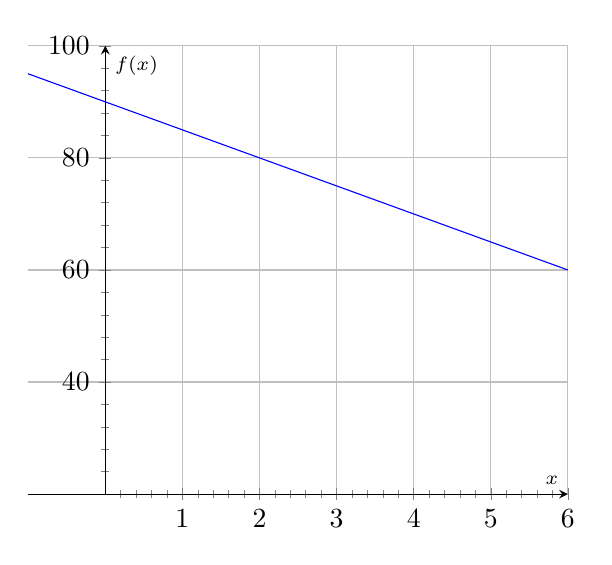
\begin{tikzpicture}[scale=1.0]
    \begin{axis}%
        [
            grid=major,
            xtick={0,1,...,7},
            minor x tick num=4, % 4 minor ticks => 5 subintervals
            xmin=-1,
            xmax=6,
            xlabel={\scriptsize $x$},
            axis x line=middle,
            ytick={20,40,...,100},
            minor y tick num=4,  % 4 minor ticks => 5 subintervals
            ymin=20,
            ymax=100,
            ylabel={\scriptsize $f(x)$},
            axis y line=middle,
            no markers,
            samples=100,
            domain=-6:6,
        ]
        \addplot[blue] (x,{-5*x+90});
    \end{axis}
\end{tikzpicture}
\break
\newpage
\subsection{Exponentielles Modell}

\subsubsection{Wachstum}
\hfill \break
Jemand hat 25€ am Spaarbuch und bekommt Wöchentich 3\% vom Ersparten dazu.
\hfill \break
$K(t)=\textcolor{red}{25}*\textcolor{blue}{1.03}^t$

\begin{itemize}
    \item \textcolor{red}{25}: Startwert
    \item \textcolor{blue}{1.05}: Wachstrumsfaktor
\end{itemize}

\hfill \break
Darstellung:\\
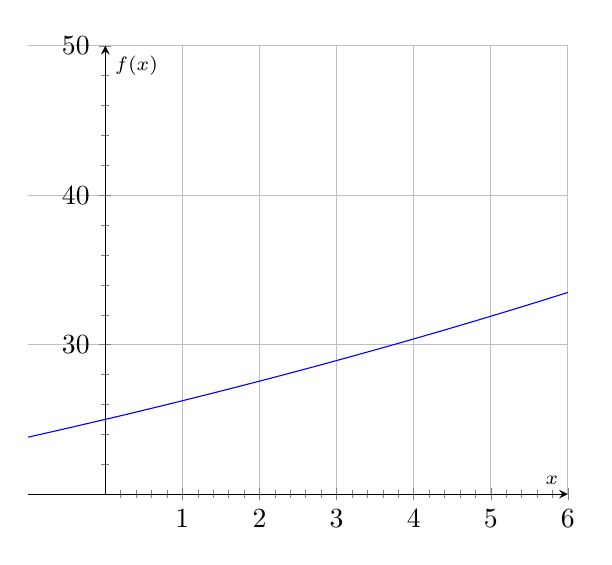
\begin{tikzpicture}[scale=1.0]
    \begin{axis}%
        [
            grid=major,
            xtick={0,1,...,7},
            minor x tick num=4, % 4 minor ticks => 5 subintervals
            xmin=-1,
            xmax=6,
            xlabel={\scriptsize $x$},
            axis x line=middle,
            ytick={10,20,...,50},
            minor y tick num=4,  % 4 minor ticks => 5 subintervals
            ymin=20,
            ymax=50,
            ylabel={\scriptsize $f(x)$},
            axis y line=middle,
            no markers,
            samples=100,
            domain=-6:6,
        ]
        \addplot[blue] (x,{25*1.05^x});
    \end{axis}
\end{tikzpicture}

\newpage
\subsubsection{Zerfall}

\hfill \break
Auf einem Konto Liegen 90€. Es werden monatlich 20\% abgehoben.
\hfill \break
$K(t)=\textcolor{red}{90}*\textcolor{blue}{0.80}^t$

\begin{itemize}
    \item \textcolor{red}{25}: Startwert
    \item \textcolor{blue}{0.80}: Zerfallsfaktor
\end{itemize}

\hfill \break
Darstellung:\\
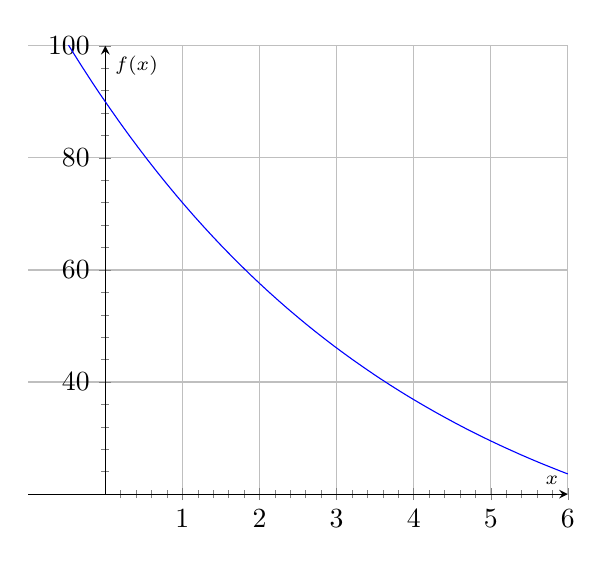
\begin{tikzpicture}[scale=1.0]
    \begin{axis}%
        [
            grid=major,
            xtick={0,1,...,7},
            minor x tick num=4, % 4 minor ticks => 5 subintervals
            xmin=-1,
            xmax=6,
            xlabel={\scriptsize $x$},
            axis x line=middle,
            ytick={20,40,...,100},
            minor y tick num=4,  % 4 minor ticks => 5 subintervals
            ymin=20,
            ymax=100,
            ylabel={\scriptsize $f(x)$},
            axis y line=middle,
            no markers,
            samples=100,
            domain=-6:6,
        ]
        \addplot[blue] (x,{90*0.80^x});
    \end{axis}
\end{tikzpicture}

\break
\newpage
\section{Trigonometry}

\hfill \break
\subsection{Strahlensatz}

\hfill \break
Werden zwei von einem Punkt ausgehende Strahlen von zwei Parallellen Geschnitten, so lassen sich daraus bestimmte Verhältnisse abslesen. $\rightarrow$ Strahlensätze


\hfill \break
Regeln:
\begin{itemize}
    \item $a:b=c:d$
    \item $b*c=a*d$
\end{itemize}


\hfill \break
Beispiel für Strahlensätze:

\hfill \break
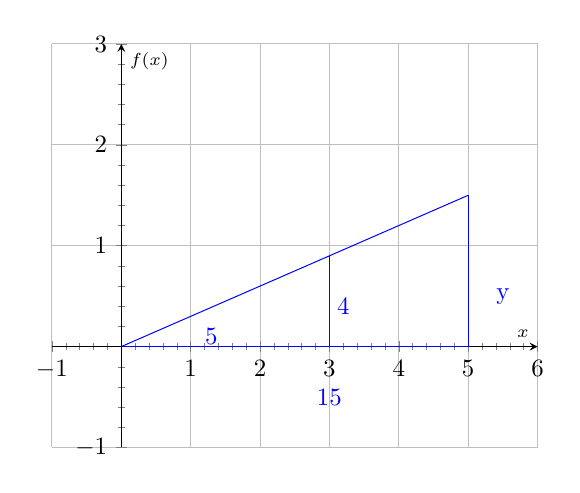
\begin{tikzpicture}[scale=0.9]
    \begin{axis}%
        [
            grid=major,
            xtick={-1,0,...,7},
            minor x tick num=4, % 4 minor ticks => 5 subintervals
            xmin=-1,
            xmax=6,
            xlabel={\scriptsize $x$},
            axis x line=middle,
            ytick={-1,0,...,3},
            minor y tick num=4,  % 4 minor ticks => 5 subintervals
            ymin=-1,
            ymax=3,
            ylabel={\scriptsize $f(x)$},
            axis y line=middle,
            no markers,
            samples=100,
            domain=-6:6,
        ]

        \draw[color=blue] (0,0) -- (5,1.5);
        \draw[color=blue] (5,0) -- (5,1.5);
        \draw[color=blue] (5,0) -- (0,0);
        \draw[color=blue] (3,0) -- (3,0.9);
        \node[color=blue] at (1.3,0.1) {5};
        \node[color=blue] at (3,-0.5) {15};
        \node[color=blue] at (5.5,0.5) {y};
        \node[color=blue] at (3.2,0.4) {4};
    \end{axis}
\end{tikzpicture}

\hfill \break
Example Verhältnisgleichung:\\
\fboxrule=0.8pt \fcolorbox{black}{lightgray}{%
    \begin{tabular}[t]{@{}l@{}}
        $5:4 = 15:y$ \\
        $5y = 60$    \\
        $y = 12$     \\
    \end{tabular}}

\break
\newpage
\subsection{Decimal und Sexagesimalsystem}

\hfill \break
\fboxrule=0.8pt \fcolorbox{lightgray}{lightgray}{%
    \begin{tabular}{c||c}
        \textcolor{red}{Decimal (Basis 10)} & \textcolor{blue}{Sexagesimal (Basis 60)} \\
        \hline
        $6.5$ h                             & 6h 30min                                 \\
        $20.1$ h                            & 20h 6min                                \\
        $19.815$ h                          & 19h 48min                                \\
    \end{tabular}}\\


\hfill \break
Umrechnung von Grad zu Rad
\begin{itemize}
    \item Grad einegben zb: $19.815$
    \item $2nd$ Angle
    \item Punkt 4 $\rightarrow$ DMS
\end{itemize}

\hfill \break
Umrechnung von Rad zu Grad
\begin{itemize}
    \item Rad einegben zb: $19^{\circ}48'54"$ die einheiten $^{\circ}$ ' können unter $2nd$ Angl gefunden werden
    \item das Zeichen " gibt es unter Alpha +
\end{itemize}

\break
\newpage
\subsection{Bogenmaß}

Das Bogenmaß ist ein Winkelmaß.\\
Das Bogenmaß eines Winkels entspricht dem Verhältnis aus Bogenlänge zum Radius.

\hfill \break
\begin{itemize}
    \item Gradmaß $ \rightarrow * \frac{\pi}{180} \rightarrow $ Bogenmaß
    \item Bogenmaß $ \rightarrow : \frac{\pi}{180} \rightarrow $ Gradmaß
    \item Bogenmaß $ \rightarrow * \frac{180}{\pi} \rightarrow $ Gradmaß
\end{itemize}


\hfill \break
Example:\\
\fboxrule=0.8pt \fcolorbox{black}{lightgray}{%
    \begin{tabular}[t]{@{}l@{}}
        $\frac{\pi}{3}rad = 60^o$ \\
        \\
        $45^o = 45 *\frac{\pi}{180} = \frac{5*\pi}{20} = \frac{\pi}{4}$\\
    \end{tabular}}
\break
\newpage
\subsection{Sinus, Cosinus und Tangens}

\hfill \break
Der Einheitskreis ist ein Kreis mir einem Radius von der Länge 1. Es wird keine Einheit angegeben.

\hfill \break
\begin{itemize}
    \item $Sin(\alpha) = \frac{\textcolor{red}{3}}{\textcolor{purple}{5}} = \frac{\textcolor{cyan}{6}}{\textcolor{violet}{7.5}}= \frac{\textcolor{cyan}{Gegenkatete}}{\textcolor{violet}{Hypothenuse}}$
    \item $Cos(\alpha) = \frac{\textcolor{green}{4}}{\textcolor{purple}{5}} = \frac{\textcolor{olive}{8}}{\textcolor{violet}{7.5}}= \frac{\textcolor{olive}{Ankatete}}{\textcolor{violet}{Hypothenuse}}$
    \item $Tan(\alpha) = \frac{\textcolor{red}{3}}{\textcolor{green}{4}} = \frac{\textcolor{cyan}{6}}{\textcolor{olive}{8}} = \frac{\textcolor{cyan}{Gegenkatete}}{\textcolor{olive}{Ankatete}}$
\end{itemize}


\hfill \break
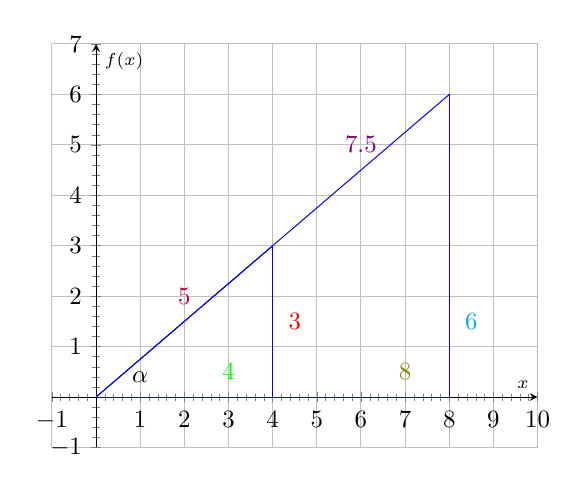
\begin{tikzpicture}[scale=0.9]
    \begin{axis}%
        [
            grid=major,
            xtick={-1,0,...,10},
            minor x tick num=4, % 4 minor ticks => 5 subintervals
            xmin=-1,
            xmax=10,
            xlabel={\scriptsize $x$},
            axis x line=middle,
            ytick={-1,0,...,7},
            minor y tick num=4,  % 4 minor ticks => 5 subintervals
            ymin=-1,
            ymax=7,
            ylabel={\scriptsize $f(x)$},
            axis y line=middle,
            no markers,
            samples=100,
            domain=-6:6,
        ]

        \draw[color=blue] (0,0) -- (8,6);
        \draw[color=blue] (0,0) -- (4,3);
        \draw[color=blue] (8,0) -- (8,6);
        \draw[color=blue] (4,0) -- (4,3);
        \draw[color=blue] (4,0) -- (0,0);
        \draw[color=blue] (8,0) -- (0,0);

        \node[color=black] at (1,0.4) {$\alpha$};

        \node[color=purple] at (2,2) {$5$};
        \node[color=violet] at (6,5) {$7.5$};
        \node[color=red] at (4.5,1.5) {$3$};
        \node[color=cyan] at (8.5,1.5) {$6$};
        \node[color=green] at (3,0.5) {$4$};
        \node[color=olive] at (7,0.5) {$8$};
    \end{axis}
\end{tikzpicture}


\hfill \break
Die Umkehrung vom Sinus ist der Arkussinus.


\hfill \break
Example zum errechnen von $\alpha$:\\
\fboxrule=0.8pt \fcolorbox{black}{lightgray}{%
    \begin{tabular}[t]{@{}l@{}}
        $Sin(\alpha) = 0.6$ // Te $\rightarrow$ $sin^{-1}$ \\
        $\alpha = 36.87^{\circ}$                           \\
        \\
        \\
        $Cos(\alpha) = 0.8$ // Te $\rightarrow$ $cos^{-1}$ \\
        $\alpha = 36.87^{\circ}$
    \end{tabular}}

\break
\newpage
\subsection{Die Winkelfunktionen}

\hfill \break
\begin{itemize}
    \item $Sin(\alpha) = \frac{GK}{H} = \frac{GK}{1} = GK$
    \item $Cos(\alpha) = \frac{AK}{H} = \frac{AK}{1} = AK$
    \item 
    \item $Tan(\alpha) = \frac{GK}{AK} = \frac{\frac{sin(\alpha)}{cos(\alpha)}}{AK}$
\end{itemize}

\hfill \break
\begin{enumerate}
    \item Trigonometriesche Grundbeziehung = $\frac{tan(\alpha)}{1} = \frac{sin(\alpha)}{cos(\alpha)}$
    \item Pythagoras = $1 = sin(\alpha)^2 + cos(\alpha)^2$
\end{enumerate}



\hfill \break
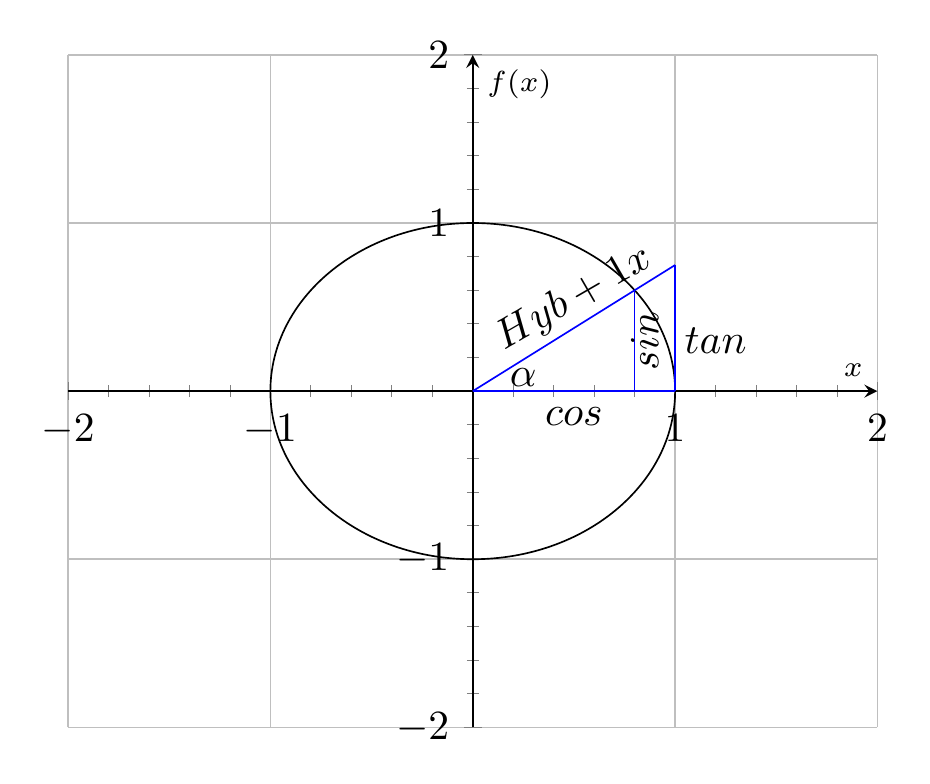
\begin{tikzpicture}[scale=1.5]
    \begin{axis}%
        [
            grid=major,
            xtick={-2,-1,...,2},
            minor x tick num=4,
            xmin=-2,
            xmax=2,
            xlabel={\scriptsize $x$},
            axis x line=middle,
            ytick={-2,-1,...,2},
            minor y tick num=4, 
            ymin=-2,
            ymax=2,
            ylabel={\scriptsize $f(x)$},
            axis y line=middle,
            no markers,
            samples=100,
            domain=-6:6,
        ]

        \draw[] (0,0) circle (1);
        \draw[color=blue] (0,0) -- (0.8,0.6);
        \draw[color=blue] (0.8,0) -- (0.8,0.6);
        \draw[color=blue] (0,0) -- (0.8,0);
        \draw[color=blue] (0.8,0.6) -- (1,0.75);
        \draw[color=blue] (1,0) -- (1,0.75);
        \draw[color=blue] (0.8,0) -- (1,0);


        \node[] at (0.25,0.08) {$\alpha$};
        \node[] at (0.5,-0.15) {$cos$};
        \node[rotate=90] at (0.85,0.3) {$sin$};
        \node[] at (1.2,0.3) {$tan$};
        \node[rotate=30] at (0.5,0.55) {$Hyb + 1x$};

    \end{axis}
\end{tikzpicture}
\break
\newpage
\subsection{Schwingungen}

\hfill \break
Die Werte von Sin und Cos können nie kleiner als -1 und größers als 1 werden.\\
Überträgt man die Längen (AK/GK) mit den dazu gehörigen Winkeln in ein Koordinatensystem, erhällt man folgende Funktionsgraphen:


\hfill \break
\subsubsection{Die Sinus Funktion}

\begin{itemize}
    \item $sin(deg(x))$
    \item diese Funktion hat eine Periode von $2*\pi$
\end{itemize}


\hfill \break
Die Wertetabelle und Graphik zu $sin(deg(x))$:\\
\fboxrule=0.8pt \fcolorbox{lightgray}{lightgray}{%
    \begin{tabular}{c|c}
        $x$               & $y$ \\
        \hline
        $0$               & 0   \\
        $\frac{\pi}{2}$   & 1   \\
        $\pi$             & 0   \\
        $\frac{3*\pi}{2}$ & -1  \\
        $2*\pi$           & 0   \\
    \end{tabular}}\\


\hfill \break
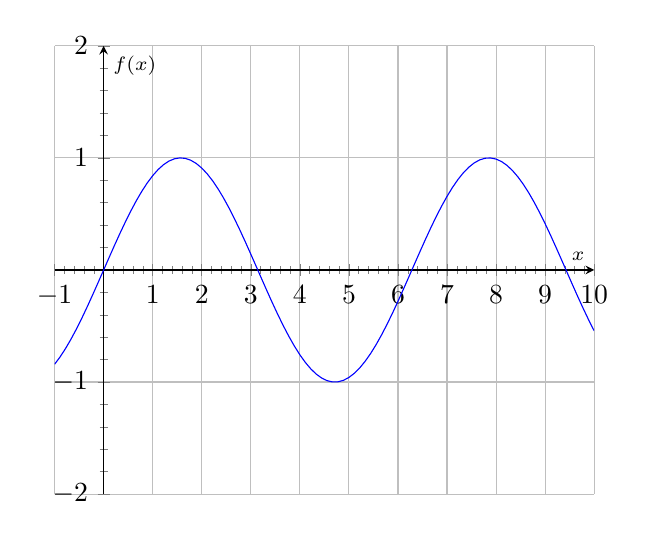
\begin{tikzpicture}[scale=1]
    \begin{axis}%
        [
            grid=major,
            xtick={-1,0,...,10},
            minor x tick num=4,
            xmin=-1,
            xmax=10,
            xlabel={\scriptsize $x$},
            axis x line=middle,
            ytick={-2,-4,...,2},
            minor y tick num=4,
            ymin=-2,
            ymax=2,
            ylabel={\scriptsize $f(x)$},
            axis y line=middle,
            no markers,
            samples=100,
            domain=-1:10,
        ]
        \addplot[blue] (x,{sin(deg(x))});
    \end{axis}
\end{tikzpicture}
\break
\newpage
\subsubsection{Die Kosinus Funktion}

\begin{itemize}
    \item $cos(deg(x))$
    \item diese Funktion hat eine Periode von $2*\pi$
\end{itemize}


\hfill \break
Die Wertetabelle und Graphik zu $cos(deg(x))$:\\
\fboxrule=0.8pt \fcolorbox{lightgray}{lightgray}{%
    \begin{tabular}{c|c}
        $x$               & $y$ \\
        \hline
        $0$               & 1   \\
        $\frac{\pi}{2}$   & 0   \\
        $\pi$             & -1   \\
        $\frac{3*\pi}{2}$ & 0  \\
        $2*\pi$           & 1   \\
    \end{tabular}}\\


\hfill \break
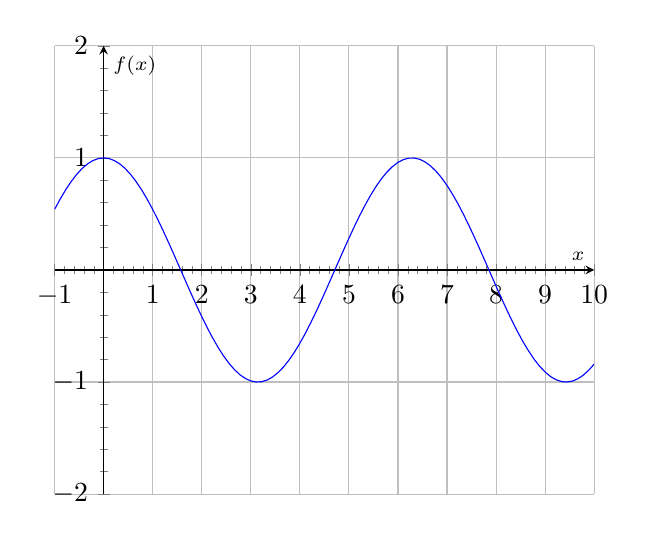
\begin{tikzpicture}[scale=1]
    \begin{axis}%
        [
            grid=major,
            xtick={-1,0,...,10},
            minor x tick num=4,
            xmin=-1,
            xmax=10,
            xlabel={\scriptsize $x$},
            axis x line=middle,
            ytick={-2,-4,...,2},
            minor y tick num=4,
            ymin=-2,
            ymax=2,
            ylabel={\scriptsize $f(x)$},
            axis y line=middle,
            no markers,
            samples=100,
            domain=-1:10,
        ]
        \addplot[blue] (x,{cos(deg(x))});
    \end{axis}
\end{tikzpicture}
\break
\newpage
\subsubsection{Die Tangens Funktion}

\begin{itemize}
    \item $tan(deg(x))$
    \item Tangens ist ein Sonderfall bezüglich des Vorzeichens.
\end{itemize}


\hfill \break
Die Wertetabelle und Graphik zu $tan(deg(x))$:\\
\fboxrule=0.8pt \fcolorbox{lightgray}{lightgray}{%
    \begin{tabular}{c|c}
        $x$               & $y$ \\
        \hline
        $0$               & 0   \\
        $\frac{\pi}{2}$   & n.d.   \\
        $\pi$             & 0   \\
        $\frac{3*\pi}{2}$ & n.d.   \\
        $2*\pi$           & 0   \\
    \end{tabular}}\\


\hfill \break
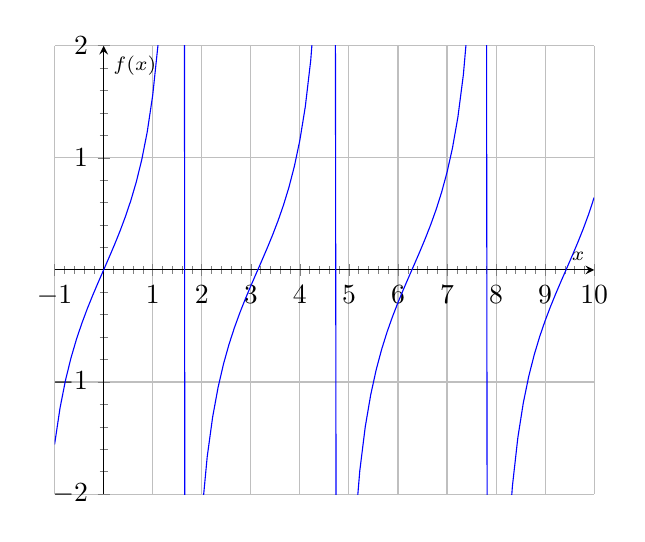
\begin{tikzpicture}[scale=1]
    \begin{axis}%
        [
            grid=major,
            xtick={-1,0,...,10},
            minor x tick num=4,
            xmin=-1,
            xmax=10,
            xlabel={\scriptsize $x$},
            axis x line=middle,
            ytick={-2,-4,...,2},
            minor y tick num=4,
            ymin=-2,
            ymax=2,
            ylabel={\scriptsize $f(x)$},
            axis y line=middle,
            no markers,
            samples=100,
            domain=-1:10,
        ]
        \addplot[blue] (x,{tan(deg(x))});
    \end{axis}
\end{tikzpicture}
\break
\newpage
\subsection{Veränderung der Sin Funktion}

\hfill \break
\subsubsection{Amplitude}

\hfill \break
Die Amplitude beschreibt die Streckung bez Stauchung entlang der $y$ Achse.
Das bedeuted das die Steigung der Funktion sinkt oder steigt.

\hfill \break
\begin{itemize}
    \item Grund-Sin Funktion $\rightarrow$ \textcolor{red}{$sin(deg(x))$}
    \item Erhöhung der Amplitude $\rightarrow$ \textcolor{green}{$2*sin(deg(x))$}
    \item Verminderung der Amplitude $\rightarrow$ \textcolor{blue}{$0.5*sin(deg(x))$}
\end{itemize}


\hfill \break
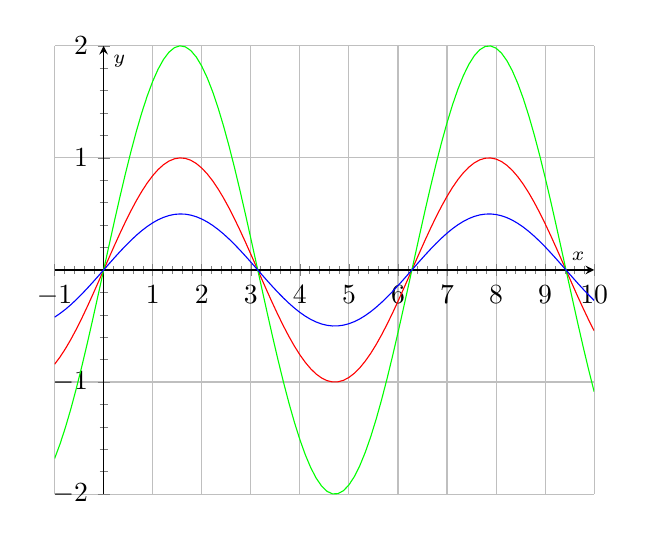
\begin{tikzpicture}[scale=1]
    \begin{axis}%
        [
            grid=major,
            xtick={-1,0,...,10},
            minor x tick num=4,
            xmin=-1,
            xmax=10,
            xlabel={\scriptsize $x$},
            axis x line=middle,
            ytick={-2,-4,...,2},
            minor y tick num=4,
            ymin=-2,
            ymax=2,
            ylabel={\scriptsize $y$},
            axis y line=middle,
            no markers,
            samples=100,
            domain=-1:10,
        ]
        \addplot[red] (x,{sin(deg(x))});
        \addplot[green] (x,{2*sin(deg(x))});
        \addplot[blue] (x,{0.5*sin(deg(x))});
    \end{axis}
\end{tikzpicture}
\break
\newpage
\subsubsection{Frequenz}

\hfill \break
Die Frequenz beschreibt die Streckung bez Stauchung entlang der $x$ Achse.
Das bedeuted das die Periode der Funktion sinkt oder steigt.

\hfill \break
\begin{itemize}
    \item Grund-Sin Funktion $\rightarrow$ \textcolor{red}{$sin(deg(x))$}
    \item Erhöhung der Frequenz $\rightarrow$ \textcolor{green}{$sin(deg(\frac{x}{2}))$}
    \item Verminderung der Frequenz $\rightarrow$ \textcolor{blue}{$sin(deg(2*x))$}
\end{itemize}


\hfill \break
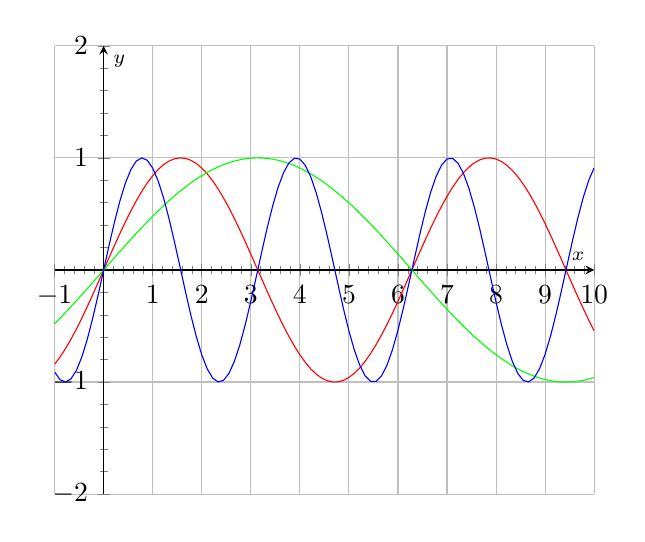
\begin{tikzpicture}[scale=1]
    \begin{axis}%
        [
            grid=major,
            xtick={-1,0,...,10},
            minor x tick num=4,
            xmin=-1,
            xmax=10,
            xlabel={\scriptsize $x$},
            axis x line=middle,
            ytick={-2,-4,...,2},
            minor y tick num=4,
            ymin=-2,
            ymax=2,
            ylabel={\scriptsize $y$},
            axis y line=middle,
            no markers,
            samples=100,
            domain=-1:10,
        ]
        \addplot[red] (x,{sin(deg(x))});
        \addplot[green] (x,{sin(deg(0.5*x))});
        \addplot[blue] (x,{sin(deg(2*x))});
    \end{axis}
\end{tikzpicture}
\break
\newpage
\subsubsection{Phasenverschiebung}

\hfill \break
\begin{itemize}
    \item allgemein: $y=sin(deg(x+c))$
    \item wen $c > 0 \rightarrow$ verschiebung Links
    \item wen $c < 0 \rightarrow$ verschiebung Rechts
\end{itemize}

\hfill \break
\begin{itemize}
    \item Grund-Sin Funktion $\rightarrow$ \textcolor{red}{$sin(deg(x))$}
    \item Rechtsverschiebung $\rightarrow$ \textcolor{green}{$sin(deg(x - \frac{\pi}{2}))$}
    \item Linksverschiebung $\rightarrow$ \textcolor{blue}{$sin(deg(x + \frac{\pi}{2}))$}
\end{itemize}


\hfill \break
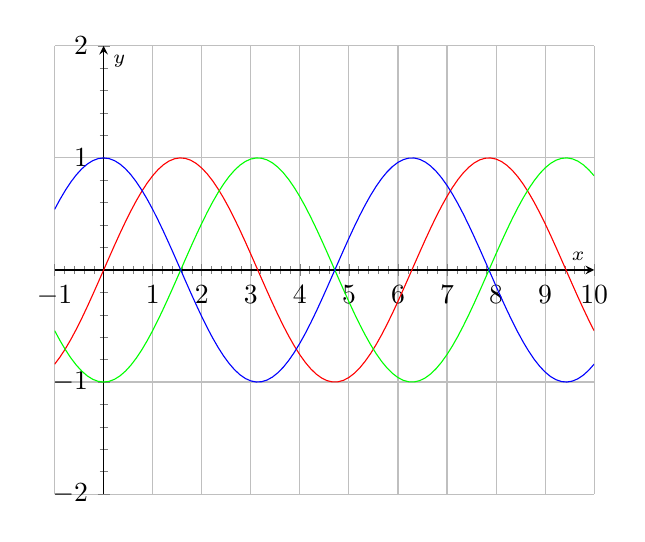
\begin{tikzpicture}[scale=1]
    \begin{axis}%
        [
            grid=major,
            xtick={-1,0,...,10},
            minor x tick num=4,
            xmin=-1,
            xmax=10,
            xlabel={\scriptsize $x$},
            axis x line=middle,
            ytick={-2,-4,...,2},
            minor y tick num=4,
            ymin=-2,
            ymax=2,
            ylabel={\scriptsize $y$},
            axis y line=middle,
            no markers,
            samples=100,
            domain=-1:10,
        ]
        \addplot[red] (x,{sin(deg(x))});
        \addplot[green] (x,{sin(deg(x - (pi / 2)))});
        \addplot[blue] (x,{sin(deg(x + (pi / 2))))});
    \end{axis}
\end{tikzpicture}

\break
\newpage
\subsection{Sinus und Kosinussatz und Fläche}

\hfill \break
In jedem Dreieck verhalten sich die Längen zweier Seiten wie die Sienuswerte der gegenüberliegenden Winkel.

\hfill \break
\begin{itemize}
    \item 1.Sinussatz $\rightarrow \frac{sin(\alpha)}{a}$
    \item 2.Sinussatz $\rightarrow \frac{sin(\beta)}{b}$
    \item 3.Sinussatz $\rightarrow \frac{sin(\gamma)}{c}$
    \item 1.Kosinussatz $\rightarrow c^2 = a^2 + b^2 +2*a*b*cos(\gamma)$
    \item 2.Kosinussatz $\rightarrow b^2 = a^2 + c^2 +2*a*c*cos(\beta)$
    \item 3.Kosinussatz $\rightarrow a^2 = b^2 + c^2 +2*b*c*cos(\alpha)$
    \item Fläche im algemeinen Dreieck $\rightarrow A = \frac{a*ha}{2}$
    \item Fläche im algemeinen Dreieck $\rightarrow A = \frac{c*b*sin(\alpha)}{2}$
\end{itemize}

\break
\newpage
\subsection{Allgemeines Dreieck}

\begin{itemize}
    \item $sin(\alpha) = \frac{hc}{b} \rightarrow hc = sin(\alpha)*b \rightarrow hc$
    \item $sin(\beta) = \frac{hc}{a} \rightarrow hc = sin(\beta)*a \rightarrow hc$
    \item $sin(\alpha)*b = sin(\beta)*a$
    \item $\frac{sin(\alpha)}{a} = \frac{sin(\beta)}{b}$
    \item $A=\frac{b*c}{2} * sin(\alpha)$
    \item $A=\frac{a*c}{2} * sin(\beta)$
    \item $A=\frac{a*b}{2} * sin(\gamma)$
\end{itemize}

\hfill \break
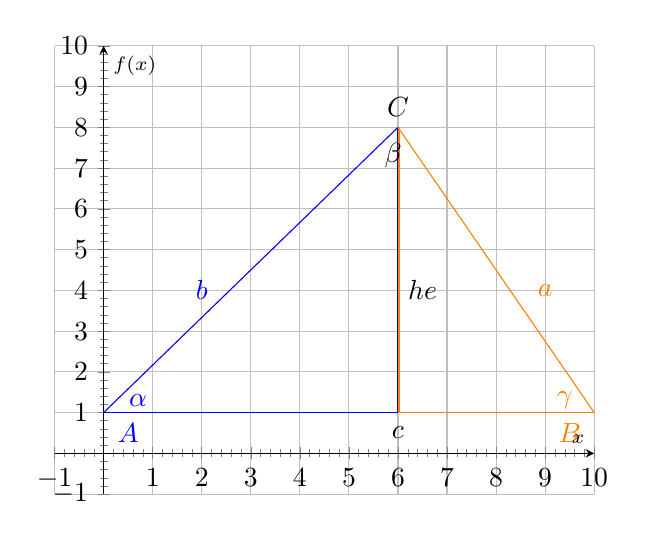
\begin{tikzpicture}[scale=1]
    \begin{axis}%
        [
            grid=major,
            xtick={-1,0,...,10},
            minor x tick num=4,
            xmin=-1,
            xmax=10,
            xlabel={\scriptsize $x$},
            axis x line=middle,
            ytick={-1,0,...,10},
            minor y tick num=4,
            ymin=-1,
            ymax=10,
            ylabel={\scriptsize $f(x)$},
            axis y line=middle,
            no markers,
            samples=100,
            domain=-1:10,
        ]

        \draw[color=blue] (0,1) -- (6,8);
        \draw[color=blue] (0,1) -- (6,1);
        \draw[color=blue] (5.99,1) -- (5.99,8);
        \draw[color=orange] (6.02,1) -- (6.02,8);
        \draw[color=orange] (10,1) -- (6,8);
        \draw[color=orange] (6,1) -- (10,1);

        \node[color=blue] at (0.7,1.3) {$\alpha$};
        \node[color=black] at (5.9,7.3) {$\beta$};
        \node[color=orange] at (9.4,1.3) {$\gamma$};

        \node[color=black] at (6.5,4) {$he$};
        \node[color=orange] at (9,4) {$a$};
        \node[color=blue] at (2,4) {$b$};
        \node[color=black] at (6,0.5) {$c$};

        \node[color=blue] at (0.5,0.5) {$A$};
        \node[color=orange] at (9.5,0.5) {$B$};
        \node[color=black] at (6,8.5) {$C$};
    \end{axis}
\end{tikzpicture}
\break
\newpage
\subsection{Vermessungsaufgaben}


\hfill \break
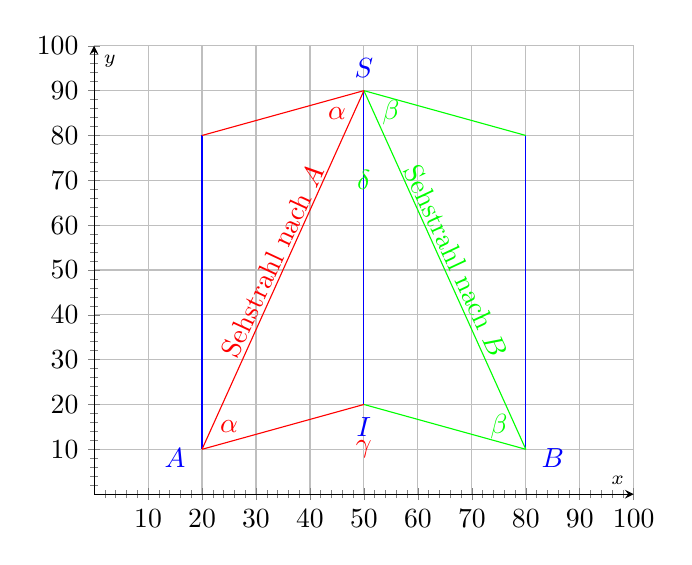
\begin{tikzpicture}[scale=1]
    \begin{axis}%
        [
            grid=major,
            xtick={0,10,...,100},
            minor x tick num=4,
            xmin=0,
            xmax=100,
            xlabel={\scriptsize $x$},
            axis x line=middle,
            ytick={0,10,...,100},
            minor y tick num=4,
            ymin=0,
            ymax=100,
            ylabel={\scriptsize $y$},
            axis y line=middle,
            no markers,
            samples=100,
            domain=-1:10,
        ]

        \draw[color=blue] (50,20) -- (50,90);
        \draw[color=blue] (20,10) -- (20,80);
        \draw[color=blue] (80,10) -- (80,80);
        \draw[color=green] (80,80) -- (50,90);
        \draw[color=green] (80,10) -- (50,20);
        \draw[color=green] (80,10) -- (50,90);
        \draw[color=red] (20,80) -- (50,90);
        \draw[color=red] (20,10) -- (50,20);
        \draw[color=red] (20,10) -- (50,90);

        \node[color=green,rotate=-65] at (67,52) {Sehstrahl nach $B$};
        \node[color=red,rotate=65] at (33,52) {Sehstrahl nach $A$};

        \node[color=red] at (25,15) {$\alpha$};
        \node[color=green] at (75,15) {$\beta$};
        \node[color=red] at (45,85) {$\alpha$};
        \node[color=green] at (55,85) {$\beta$};

        \node[color=red] at (50,10) {$\gamma$};
        \node[color=green] at (50,70) {$\delta$};
        \node[color=blue] at (15,8) {$A$};
        \node[color=blue] at (85,8) {$B$};
        \node[color=blue] at (50,95) {$S$};
        \node[color=blue] at (50,15) {$I$};


    \end{axis}
\end{tikzpicture}


\hfill \break
\begin{itemize}
    \item $\textcolor{red}{\alpha},\textcolor{green}{\beta} \rightarrow$ Hähenwinkel, von der Horizontale aus nach oben gemessen.
    \item $\textcolor{red}{\alpha},\textcolor{green}{\beta} \rightarrow$ Tiefenwinkel, von der Horizontale aus nach unten gemessen.
    \item $\textcolor{red}{\gamma}... Horizontalwinkel$ zwischen den 2 gedachten Linien.
    \item $\textcolor{green}{\delta}... Sehwinkel$ von 2 Sehstralen.
\end{itemize}

\newpage
\subsubsection{Beispiel 1: Der Fluss}

\hfill \break
Berechne die Breite eines Flusses, wenn in einem geradlinigen Uferstück die Standlinie AB (150m) abgesteckt wird
sowie die Winkel CAB (63°22') und CBA (44°30') zu einem am gegenüberliegenden Ufer liegenden Punkt C gemessen
wird.
(Lösung: 98,75m)

\hfill \break
\begin{itemize}
    \item Winkel $CAB = \alpha = 63.37$°
    \item Winkel $CBA = \beta = 44.5$°
    \item Winkel $BC = \gamma = 72.13$°
\end{itemize}

\hfill \break
Rechenweg:\\
\fboxrule=0.8pt \fcolorbox{black}{lightgray}{%
    \begin{tabular}[t]{@{}l@{}}
        $x = \frac{Sin(44.5)*150}{Sin(72.13)}$ \\
        $x = 110.47$                           \\
        \\
        $b=Sin(\alpha)/x$                      \\
        $b=Sin(63.37)*110.47$                  \\
        $b=98.75m$                              \\
    \end{tabular}}

\hfill \break
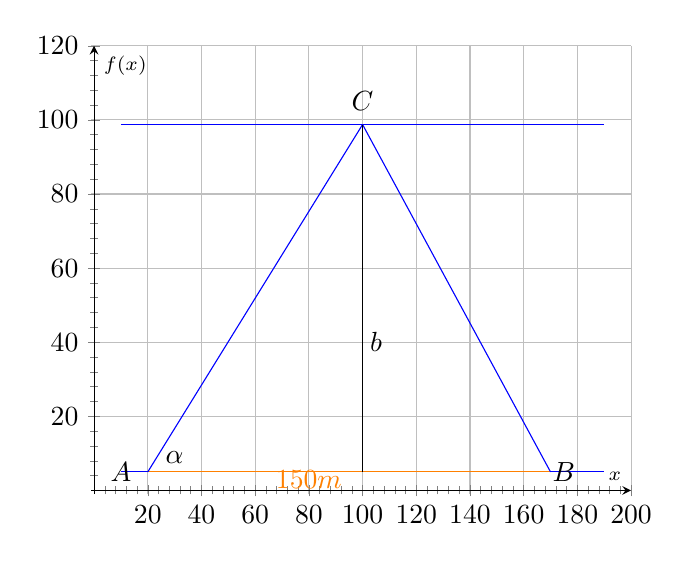
\begin{tikzpicture}[scale=1]
    \begin{axis}%
        [
            grid=major,
            xtick={0,20,...,200},
            minor x tick num=4,
            xmin=-1,
            xmax=200,
            xlabel={\scriptsize $x$},
            axis x line=middle,
            ytick={0,20,...,120},
            minor y tick num=4,
            ymin=-1,
            ymax=120,
            ylabel={\scriptsize $f(x)$},
            axis y line=middle,
            no markers,
            samples=100,
            domain=-1:10,
        ]

        \draw[color=blue] (10,5) -- (190,5);
        \draw[color=orange] (20,5) -- (170,5);
        \draw[color=blue] (10,98.75) -- (190,98.75);
        \draw[color=blue] (100,98.75) -- (20,5);
        \draw[color=blue] (100,98.75) -- (170,5);
        \draw[color=black] (100,98.75) -- (100,5);

        \node[color=black] at (10,5) {$A$};
        \node[color=black] at (175,5) {$B$};
        \node[color=black] at (100,105) {$C$};
        \node[color=black] at (105,40) {$b$};
        \node[color=black] at (30,9) {$\alpha$};
        \node[color=orange] at (80,3) {$150m$};
    \end{axis}
\end{tikzpicture}
\newpage
\subsubsection{Beispiel 2: Der Antennemast}

\hfill \break
Der Antennenmast eines Fernsehturms hat die Höhe h = 75m. Von einem Geländepunkt P werden Spitze und Fußpunkt
des Antennenmast unter den Höhenwinkeln a = 24°12' und ß = 17°42' gesehen. Ermittle die Höhe des Fernsehturms
mit Sendemast.
(Lösung: 258,73m)

\hfill \break
\begin{itemize}
    \item Winkel $\alpha = 24.2$°
    \item Winkel $\beta = 17+\frac{42}{60}$°
    \item Winkel $\gamma = 24.2-1.7=6.5$°
    \item Winkel $\delta = 180 - 90 - 17.7 = 72.3$°
    \item Winkel $\epsilon = 107.7$°
    \item Winkel $\zeta = 65.8$°
\end{itemize}

\hfill \break
Rechenweg:\\
\fboxrule=0.8pt \fcolorbox{black}{lightgray}{%
    \begin{tabular}[t]{@{}l@{}}
        $\frac{75}{Sin(\alpha)} = \frac{\gamma}{Sin(\zeta)}$ \\
        $\frac{75}{Sin(\alpha)} = \gamma$                    \\
        $y = 604.3$                                          \\
        \\
        $Sin(\beta) = \frac{x}{y}$                           \\
        $Sin(\beta)*\gamma = x$                              \\
        $x = 183.73$                                         \\
        \\
        $H = 183.73 + 75 = 258.73$                           \\
    \end{tabular}}

%//TODO add drawing
\break
\newpage
\section{Änderungsmaße}

\hfill \break
Die Änderungsmaße beschreiben eine Änderung von Werten über eine Zeitspanne (zb.: $2004-2015$).

\begin{itemize}
    \item Im Jahre $2009$ = $17154$ Geburten
    \item Im Jahre $2010$ = $17989$ Geburten
    \item Im Jahre $2011$ = $18170$ Geburten
    \item Im Jahre $2012$ = $18265$ Geburten
    \item
    \item Absolute Änderung: $18265-17154 = 1111$ Geburten
    \item Mittlere Änderung: $\frac{18265-17154}{3} \cong 370$ Geburten/jahr
    \item Relative Änderung: $\frac{1111}{17154} = 0.065 = 6.5\%$
\end{itemize}


\hfill \break
\break
\subsection{Beispiele}

\hfill \break
Eine Firma macht im Monat meinen Umsatz U(m). Interpretiere den gegebenen Ausdruck im Kontext.
\begin{itemize}
    \item $U(m)-U(n) >0$ : Es wurde Gewinn im vergleich zum Vorjar erwirtschaftet.
    \item $\frac{U(m)-U(n)}{U(n)} = 12$ : Der Umsatz hat um 12\% zugenommen.
\end{itemize}


\break
\newpage
\section{Differentialgleichung}

Wichtige ableitungen:
\begin{enumerate}
    \item Potenz-funktionen \begin{itemize}
              \item $f(x) = x^n$
              \item $f'(x) = n*x^{n-1}$
          \end{itemize}
    \item Exponentialfunktionen \begin{itemize}
              \item $f(x) = e^x$
              \item $f'(x) = e^x$
              \item $f(x) = a^x$
              \item $f'(x) = a^x * ln(a)$
          \end{itemize}
    \item Logarithmusfunktion \begin{itemize}
              \item $f(x) = ln(x)$
              \item $f'(x) = \frac{1}{x}$
          \end{itemize}
    \item Trigonometrische Funktionen \begin{itemize}
              \item $f(x) = sin(x)$
              \item $f'(x) = cos(x)$
              \item $f(x) = cos(x)$
              \item $f'(x) = -sin(x)$
              \item $f(x) = tan(x)$
              \item $f'(x) = \frac{1}{cos^2(x)}$
          \end{itemize}
\end{enumerate}

\newpage
\newpage
\subsection{Differenzenquotient - MITTLERE Änderungsrate}

\hfill \break
Die Ableitung von f an der Stelle x ist der Anstieg der Tangente an den Graphen von f im Punkt $(x,f(x))$. Zur
Kennzeichnung der Ableitung wird der Funktionsterm mit dem Symbol $f'(x)$ bezeichnet.
Die Ableitung einer Funktion ist selbst wieder eine Funktion= Ableitungsfunktion. Ihr Funktionswert an der
Stelle x ist $f'(x)$.

\begin{itemize}
    \item $f'(x) = 0$: Das bedeutet, dass die Tangente am Graphen an der Stelle x den Anstieg O hat, die
          Tangente ist also parallel zur x-Achse.
    \item $f'(x) > 0$: Das bedeutet, dass die Tangentensteigung positiv ist, der Graph ist monoton steigend an
          der Stelle x.
    \item $f'(x) < 0$: Das bedeutet, dass die Steigung der Tangente negativ ist und der Graph monoton fallend
          an der Stelle x ist.
\end{itemize}

\begin{enumerate}
    \item Konstante Funktionen ($f(x) = d$, $f'(x) = 0$): Der Graph einer konstanten Funktion ist
          eine Gerade, welche parallel zur x-Achse
          verläuft. Die Steigung ist in jedem Punkt x
          gleich Null!
    \item Lineare Funktionen ($f(x) = kx + d$, $f'(x) = k$): Der Graph der linearen Funktion ist eine
          Gerade mit Anstieg k. Die Steigung ist in
          jedem Punkt k!
\end{enumerate}

\hfill \break
Geometrische Interpretation der mittleren Änderungsrate:\\
Aus der Sekante wird eine Tangente. Der Punkt B geht
in Punkt A über, somit wird $\Delta x$ immer kleiner und
kleiner, es geht somit gegen Null $(\Delta x \rightarrow 0)$.

\hfill \break
Anstieg der Kurve in einem Punkt = Steigung der Tangente:\\
$lim_{\Delta x \rightarrow 0}(\frac{f(b)-f(a)}{\Delta x}) = f'(x) = 1$ = 1. Ableitung von f nach x

\hfill \break
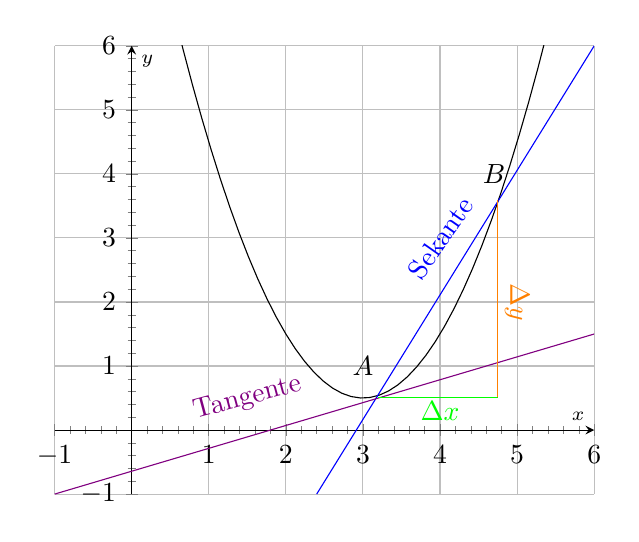
\begin{tikzpicture}[scale=1]
    \begin{axis}%
        [
            grid=major,
            xtick={-1,0,...,7},
            minor x tick num=4, % 4 minor ticks => 5 subintervals
            xmin=-1,
            xmax=6,
            xlabel={\scriptsize $x$},
            axis x line=middle,
            ytick={-1,0,...,7},
            minor y tick num=4,  % 4 minor ticks => 5 subintervals
            ymin=-1,
            ymax=6,
            ylabel={\scriptsize $y$},
            axis y line=middle,
            no markers,
            samples=100,
            domain=-6:6,
        ]
        \addplot[black] (x,{0.5+(x-3)^2});
        \draw[blue] (6,6) -- (2.4,-1);
        \draw[violet] (-1,-1) -- (6,1.5);
        \draw[orange] (4.75,3.6) -- (4.75,0.51);
        \node[color=blue,rotate=55] at (4,3) {Sekante};
        \node[color=violet,rotate=15] at (1.5,0.5) {Tangente};
        \node[color=orange,rotate=-90] at (5,2) {$\Delta y$};
        \draw[green] (3.2,0.51) -- (4.75,0.51);
        \node[color=green] at (4,0.3) {$\Delta x$};
        \node[color=black] at (3,1) {$A$};
        \node[color=black] at (4.7,4) {$B$};
    \end{axis}
\end{tikzpicture}
\hfill \break
\newpage
\subsection{Weg, Geschwindigkeit und Beschleunigung}

\fboxrule=0.8pt \fcolorbox{lightgray}{lightgray}{%
    \begin{tabular}{c|c|c}
        Weg   & Geschwindigkeit       & Beschleunigung                  \\
        S     & V                     & a                               \\
        Meter & Veränderung des Weges & Veränderung der Geschwindigkeit \\
        $km$  & $m/s$   $km/h$        & $m/s^2$   $km/h^2$              \\
    \end{tabular}}\\

\hfill \break
\begin{itemize}
    \item Ableiten: $s(t) \rightarrow v(t) \rightarrow a(t)$
    \item Integrieren: $a(t) \rightarrow v(t) \rightarrow s(t)$
\end{itemize}

\hfill \break
Wichtige Formeln:
\begin{itemize}
    \item $S=V*t$
    \item $f'(x)=k$
\end{itemize}

\break
\section{Ableitungen}

Regeln:\\
\begin{itemize}
    \item Produktregel: $f'*g+f*g'$
    \item Kettenregel: algemein: $\textcolor{red}{g(}f(x\textcolor{red}{)} = \textcolor{red}{g'(}f(x)\textcolor{red}{)}*f'(x)$\\
          $y=\textcolor{red}{(}x^2\textcolor{red}{)^3} \rightarrow y'=\textcolor{red}{3*(}x^2\textcolor{red}{)^2} \rightarrow y'=6x*(x^2)^2 = 6x^5$
    \item Potenzregel: $y=\sqrt{x} = x^\frac{1}{2} \rightarrow \frac{1}{2}*x^{-\frac{1}{2}} = \frac{1}{2}*\frac{1}{x^\frac{1}{2}} = \frac{1}{2\sqrt{x}}$
\end{itemize}


\hfill \break
\subsection{Graphisches Ableiten}

Zu merken:\\
\begin{itemize}
    \item Das Maximum bzw. Minimum von $f(x)$ wird in der Ableitungsfunktion $f'(x)$ zur Nullstelle.
    \item Der Wendepunkt von $f(x)$ wird in der Ableitungsfunktion $f'(x)$ zum Minnimum und Maximum.
    \item Eine positive Steigung in $f(x)$ beutet positieve Werte in $f'(x)$.
    \item Eine negative Steigung in $f(x)$ beutet negative Werte in $f'(x)$.
    \item Als Sattelpunkt bezeichnet man einen Punkt an dem die Tangente wagrecht ist das bedeutet $f(x) = 0$ und $f"(x) = 0$
    \item Beim Graphischen Ableiten wird der Sattelpunkt zur Extremstelle.
\end{itemize}
\break
\newpage
\subsection{Graphisches Ableiten Beispiele}

\hfill \break
\begin{itemize}
    \item \textcolor{blue}{Funktion}
    \item \textcolor{red}{Ableitung}
\end{itemize}

\hfill \break
Example $f(x) = 2x-1$:\\
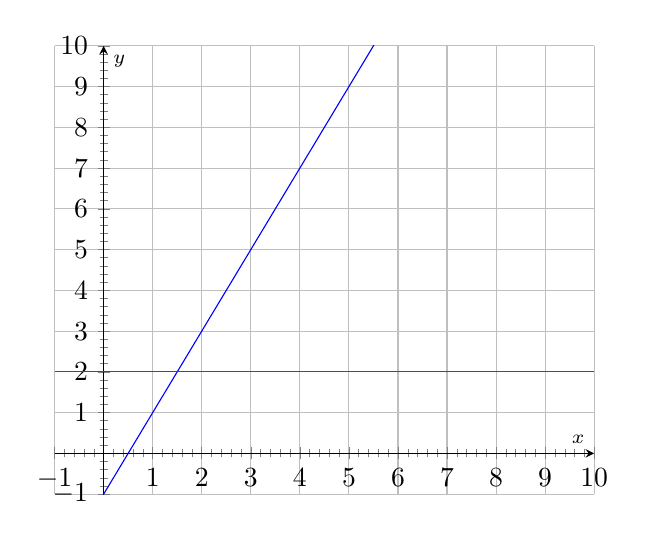
\begin{tikzpicture}[scale=1]
    \begin{axis}%
        [
            grid=major,
            xtick={-1,0,...,10},
            minor x tick num=4,
            xmin=-1,
            xmax=10,
            xlabel={\scriptsize $x$},
            axis x line=middle,
            ytick={-1,0,...,10},
            minor y tick num=4,
            ymin=-1,
            ymax=10,
            ylabel={\scriptsize $y$},
            axis y line=middle,
            no markers,
            samples=100,
            domain=-1:10,
        ]
        \addplot[blue] (x,{2*x-1});
        \addplot[red] (x,{2});
    \end{axis}
\end{tikzpicture}

\hfill \break
Example $f(x) = ((x-1)^2)-1$:\\
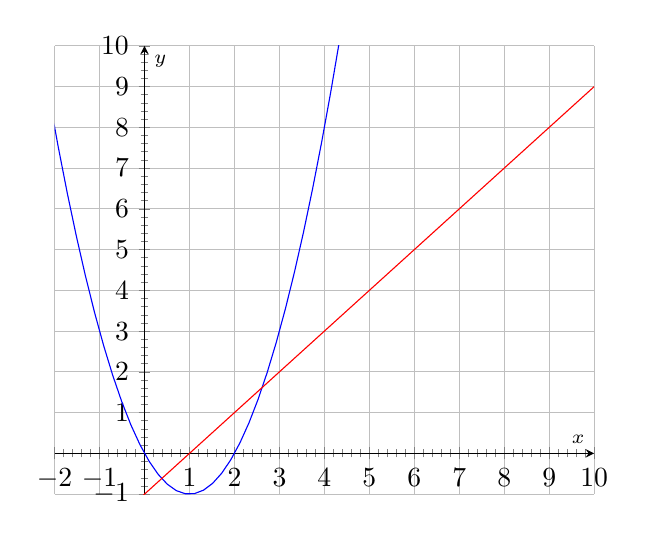
\begin{tikzpicture}[scale=1]
    \begin{axis}%
        [
            grid=major,
            xtick={-2,-1,...,10},
            minor x tick num=4,
            xmin=-2,
            xmax=10,
            xlabel={\scriptsize $x$},
            axis x line=middle,
            ytick={-1,0,...,10},
            minor y tick num=4,
            ymin=-1,
            ymax=10,
            ylabel={\scriptsize $y$},
            axis y line=middle,
            no markers,
            samples=100,
            domain=-10:10,
        ]
        \addplot[blue] (x,{((x-1)^2)-1});
        \addplot[red] (x,{2(x-1)});
    \end{axis}
\end{tikzpicture}
\break
\newpage
\subsection{Funktion Aufstellen}

Eine Parabel, die durch den Koordinatenursprung geht, hat den Scheitel S. Stelle die Gleichung der zugehörigen
quadratischen Funktion auf.\\

Anhaltspunkte:\\
\begin{itemize}
    \item $f(x) = ax^2+bx+c$
    \item $P=(0|0)$
    \item $S=(5|-6)$
    \item $f(0)=0$
    \item $f'(5)=-6$
    \item $f"(5)=0$
\end{itemize}

\begin{align*}
    f'(x) & = 2ax+b \mbox{ // hier die erste ableitung der Basis Funktion } \\
    0     & = 0a+0b+c                                                      \\
    -6    & = 25a+5b+c                                                     \\
    0     & = 10a+b                                                        \\
    f(x)  & = \frac{6}{25}x^2-\frac{12}{5}
\end{align*}
\break
\newpage
\subsection{Musterbeispiel für eine vollständige Kurvendiskussion}

Gegeben ist eine Funktion $f(x)=x^3-3x+1$ Führe eine vollständige Diskussion der Funktion durch.\\

\begin{enumerate}
    \item Die Funktion und ihre Ableitungen: \begin{itemize}
              \item $f(x)=x^3-3x+1$
              \item $f'(x) = 3x^2-3$
              \item $f''(x) = 6x$
          \end{itemize}
    \item Nullstellen ermitteln: $f(x)=0$ \begin{itemize}
              \item $x^3-3x+1=0$
              \item Zur Berechnung gibt es zwei Möglichkeiten mit dem TR: \begin{enumerate}
                        \item grafisch: $y1$ in die Liste eingeben 2nd - calc - zero ; Cursor links und rechts setzen und jeweils  mit ENTER bestätigen.\\ $N_1(-1,88|0)$; $N_2(0.35|0)$; $N_3(1.53|0)$;
                        \item SOLVER: Math - 0 - $\uparrow$ eqn: $0=x^3-3x+1$ ENTER x = Startwert eingeben (-10, 0, 10; auf Verdacht probieren) bzw. eventuell Tabelle 2nd - table nützen 
                    \end{enumerate}
          \end{itemize}
    \item Extremstellen berechnen: \begin{itemize}
        \item $f'(x)=0$
        \item $f''(x) < 0$ = Hochpunkt
        \item $f''(x) > 0$ = Tiefpunkt
        \item $3x^2-3=0$ $\rightarrow$ $3x^2=3$ $\rightarrow$ $x^2=1$ $\rightarrow$ $x = \pm 1$
        \item $f''(-1)<0$ $\rightarrow$ $f(-1)=3$ $\rightarrow$ Hochpunkt $H(-1|3)$
        \item $f''(1)>0$ $\rightarrow$ $f(1)=-1$ $\rightarrow$ Tiefpunkt $T(1|-1)$
    \end{itemize}
    \item Wendepunkt berechnen: $f''(x)=0$ \begin{itemize}
        \item $6x=0$
        \item $x=0$
        \item $f(0)=1$ Wendepunkt $W(0|1)$
    \end{itemize}
    \item Wendetangente berechnen: $t_w:y=kx+d$ \begin{itemize}
        \item $k=f'(0)=-3$
        \item $t_w:y=kx+d$
        \item $W(0|1)$ in y = $-3x+d$ einsetzen 
        \item $1=-3*0+d$
        \item $d=1$
        \item $t_w:y=-3x+1$
    \end{itemize}
\end{enumerate}



\break
\newpage
\subsection{Übersetzungshilfen zum Aufstellen von Gleichungen (Differentialrechnung)}

\begin{itemize}
    \item ... verläuft durch den Punkt $P(2|6)$ $\implies$ $f(2)=6$
    \item ... hat Nullstelle bei $x=9$ $\implies$ $f(9)=0$
    \item ... schneidet die y- Achse bei $3$ $\implies$ $f(0)=3$
    \item ... schneidet die Gerade mit $y=3x-7$ auf der y-Achse $\implies$ $f'(0)=3$
    \item ... berührt die x-Achse an der Stelle $x=5$ $\implies$ $f(5)=0$ und $f'(5)=0$ 
    \item ... hat einen Tiefpunkt bei $T(2|-7)$ $\implies$ $f(2)=-7$ und $f'(2)=0$
    \item ... hat einen Wendepunkt bei $P(-1|2)$ $\implies$ $f(-1)=2$ und $f'(-1)=0$
    \item ... besitzt im Punkt $P(2|-3)$ die Steigung 4 $\implies$ $f(2)=-3$ und $f(2)=4$
    \item ... besitzt an der Stelle $x=-2$ eine Wendetangente mit Steigung 1 $\implies$ $f''(-2)=0$ und $f'(-2)=1$
    \item ... die Tangente in $P(-1|5)$ ist parallel zur Gerade $y=6x$ $\implies$ $f(-1)=5$ und $f(-1)=6$
\end{itemize}
\break
\newpage
\subsection{Ableitung einiger anderen Funktionen}

\begin{itemize}
    \item $f(x)=\frac{1}{5}*(x^3-2x^2+7) \implies f'(x)=\frac{1}{5}*(3x^2)-4x$
    \item $f(x)=x^3*x^5 \implies f(x)=x^8 \implies f'(x)=8x^7$
    \item $f(x)=\frac{sin(x)}{f}*\frac{3x}{g} \implies f'(x)=cos(x)*3x+sin(x)*3$
    \item $f(x)=\frac{cos(x)}{x^2} \implies \frac{f'*g - f*g'}{g^2} \implies f'(x)=\frac{-sin(x)*x^2)-cos(x)*2x}{x^4} = \frac{-sin(x)*x-2*cos(x)}{x^3}$
\end{itemize}
\break
\section{Integrale}

Integralrechnung ist das Gegenteil zur Ableitung

\begin{itemize}
    \item Ableitung: $f(x) = x^2+3 \rightarrow f'(x) = 2x$
    \item Integrieren: $f(x) = x^2+3 \leftarrow f'(x) = 2x$
    \item $F(x) = \frac{2x^2}{2} = x^2+c$ wobei $c \in \mathbb{R}$        $\mathbb{R}$ ist die Integrationskonstante
    \item Stammfunktion = $\textcolor{red}{F(x)}$
    \item Algemein: $f(x) = c^n \rightarrow \textcolor{red}{F(x)} = \frac{x^{n+1}}{n+1}+c$
\end{itemize}

Man benötight eine Zusatzinformation um die Stammfunktion bcw.: $c$ eindeutig bestimmen zu können.

\hfill \break
\subsection{Anwändung Inigral}

Die Integralrechnung wird verwendetum...\\
\begin{itemize}
    \item um die Tammfuntion zu bestimmen $\rightarrow$ Das bestimmte Integral
    \item um die Fläche unter einer Funtion zu bestimmen $\rightarrow$ Das unbestimmte Integral
\end{itemize}
\break
\newpage
\subsection{Das bestimmte Integral}

Die Ableitung der Stammfunktion ergibt die Funktion selbst. $\rightarrow F'(x)=f(x)$

\hfill\break
\begin{itemize}
    \item Bestimme die Stammfunktion der Funktion $f(x)=2x$
    \item Welche Funktion ergibt abgeleitet $f(x)=2x \rightarrow F(x)=x^2$
    \item Weil $\rightarrow F'(x) = 2x = f(x)$
\end{itemize}

Eine Ableitungsregel besagt, dass eine Konstante beim Ableiten wegfällt.
Aus diesem Grund ist die oben angegebene Lösung nur eine von unendlich vielen, denn auch z.B. $F(x)=x^2+3$ und $F(x)=x^2-9$ sind Stammfunktionen von $f(x)=2x$.
Da sich die einzelnen Stammfunktionen nur durch eine Konstante $C$ unterscheiden, schreiben wir $F(x)=x^2+C$
\break
\newpage
\subsection{Das unbestimmte Integral}

Die Fläche wird immer von Nullstelle zu Nullstelle berechnet weil wen man versucht die rechn ung auf einmal
mit den taschenrechner zu lösen wird alles unter dem Nullpunkt von allem größer null subtrahieren.


$$A=\int\limits_1^7 3dx=3x+c |_1^7 = \textcolor{red}{3*7+x}-\textcolor{blue}{(3*1+c)} = 21-3 = 18$$
\begin{itemize}
    \item \textcolor{red}{obere Gänze}
    \item \textcolor{blue}{unterre Gänze}
\end{itemize}


\hfill \break
Example:\\
\fboxrule=0.8pt \fcolorbox{lightgray}{lightgray}{%
    \begin{tabular}{ |c|}
        \hline
        GrundFormel: $f(x) = -x^2+4$                                                                                                                                                                \\
        $F(x) = -\frac{x^3}{3} +4x$                                                                                                                                                                 \\
        Integral: $\int\limits_{-2}^2 f(x)dx$                                                                                                                                                       \\
        $\int\limits_{-2}^2 f(x)dx = 2*\int\limits_0^2 f(x)dx = 2*(-\frac{x^2}{3}+4 |_0^2) = 2*(\frac{2}{3}+4*2(-\frac{0^3}{3}+4*0)=2*(-\frac{8}{3}+8) = 2* \frac{16}{3} = \frac{32}{3})$ \\
        \hline
    \end{tabular}}\\

\hfill \break
\begin{itemize}
    \item Gegben: $f(x)=3$
    \item Gesucht: Flächeninhalt ($f(x)$) von $x_1=1$ bis $x_2=7$
\end{itemize}


\hfill \break
Mit dem Taschenrechner: Rechnerrisch:
\begin{enumerate}
    \item Math $\uparrow$
    \item a: fnInt
    \item fnint(3,x,\textcolor{red}{1},\textcolor{blue}{7}) $\textcolor{red}{1=x_1}$ $\textcolor{blue}{7=x_2}$
\end{enumerate}

\hfill \break
Mit dem Taschenrechner: Grafisch:
\begin{enumerate}
    \item $y_1$ = 3
    \item $2_{nd}$ calc 7. f(x)dx
\end{enumerate}


\break
\newpage
\subsection{Fläche zwischen Funktionen}

Es soll die Fläche zwischen den beiden Funktionen ermittelt werden:
\begin{itemize}
    \item $\textcolor{blue}{f(x) = x^2+2}$
    \item $\textcolor{red}{g(x) = -x^2+5}$
\end{itemize} 

\hfill \break
Schritte:
\begin{enumerate}
    \item Schnittpunkte Berechnen: \begin{itemize}
        \item Ermittlung durch Gleichsetzen: $f(x) = g(x)$
        \item Ermittlung mit TR $2_{nd}$ calc intersect
    \end{itemize}
    \item Zwischen den ermittelten Schnittpunkten Integrieren: $\int\limits_{x2}^{x1} g(x)-f(x)dx$
\end{enumerate}

\hfill \break
Dabei sit zu beachten das immer die obere minus der unterren Kurve gerechnet werden muss.

\hfill \break
Example:\\
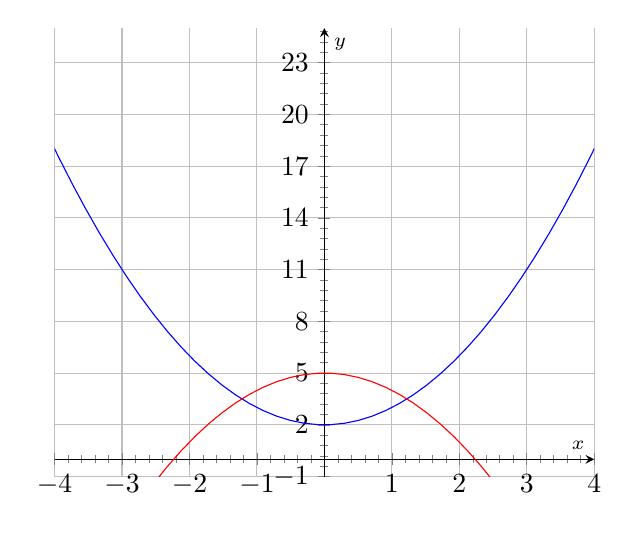
\begin{tikzpicture}[scale=1]
    \begin{axis}%
        [
            grid=major,
            xtick={-5,-4,...,4},
            minor x tick num=4,
            xmin=-4,
            xmax=4,
            xlabel={\scriptsize $x$},
            axis x line=middle,
            ytick={-1,2,...,25},
            minor y tick num=4,
            ymin=-1,
            ymax=25,
            ylabel={\scriptsize $y$},
            axis y line=middle,
            no markers,
            samples=100,
            domain=-10:10,
        ]
        \addplot[blue] (x,{x^2+2});
        \addplot[red] (x,{-x^2+5});
    \end{axis}
\end{tikzpicture}
\break
\newpage
\subsection{Kurvenschar}

Eine Kurvenschar ergiebt sich darurch das das $c$ bein intigreieren nicht bestimmt ist: $f(x)dx = F(x)+c$.\\
Und da $c \in \mathbb{R}$ wegeben sich verschiedene Möglichkeiten für $c$ was sin in den möglichen Kurven wiederspiegelt.

\hfill \break
Example:\\
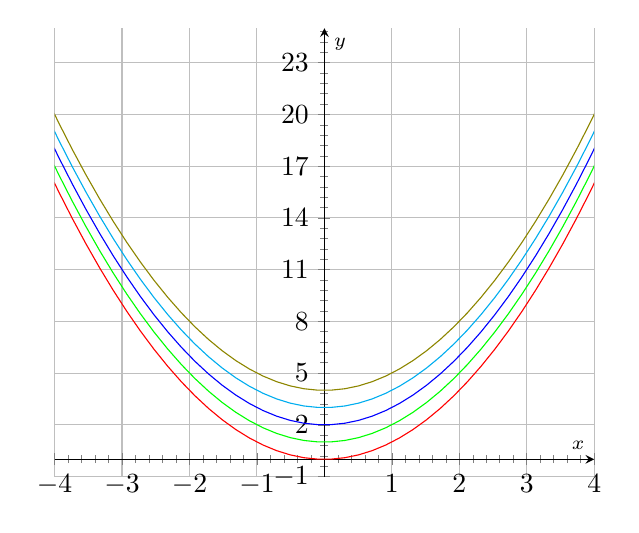
\begin{tikzpicture}[scale=1]
    \begin{axis}%
        [
            grid=major,
            xtick={-5,-4,...,4},
            minor x tick num=4,
            xmin=-4,
            xmax=4,
            xlabel={\scriptsize $x$},
            axis x line=middle,
            ytick={-1,2,...,25},
            minor y tick num=4,
            ymin=-1,
            ymax=25,
            ylabel={\scriptsize $y$},
            axis y line=middle,
            no markers,
            samples=100,
            domain=-10:10,
        ]
        \addplot[red] (x,{x^2+0});
        \addplot[green] (x,{x^2+1});
        \addplot[blue] (x,{x^2+2});
        \addplot[cyan] (x,{x^2+3});
        \addplot[olive] (x,{x^2+4});
    \end{axis}
\end{tikzpicture}

\break
\newpage
\section{Wahrscheinlichkeitsrechnung}

Wichtige Zeichen, Sybole udn Regeln:\\
\begin{itemize}
    \item $\lnot$ bedeuted soviel wie "Verneinung" oder "nicht"
    \item "oder" bedeuted soviel wie + in der Rechnung später
    \item "und" bedeuted soviel wie * in der Rechnung später
\end{itemize}


\hfill \break
Grundidee:\\
Zufallsexperiment ist das Experiment das Dem Zufall ausgesetzt ist.\\ 
Den möglichen Ausgang nennt man Ereigniss.\\
Die Menge aller Ereignisse nennt man ereignisraum Zeichen: $\Omega$.\\
$\Omega = {1,2,3,4,5,6}$ zb wäre der ereignisraum beim Würfeln eines Würfels (einmalig).

\hfill \break
Zufallsexperimente Beispiele:
\begin{itemize}
    \item Lotto
    \item Joker
    \item Münzwurf
    \item Würfeln
\end{itemize}

\hfill \break
Das Laplace Experiment:\\
Bei diesem Experiment haben alle Ereignisse die selbe Wahrscheinlichkeit:\\
zb.: das Werfen eines Würfels $P(6er) = \frac{1}{6}$ das $P$ steht dabei für den griechischen ausdruck Probabilitas.\\
\begin{itemize}
    \item $P(6er) = \frac{1}{6}$
    \item $P(4er) = \frac{1}{6}$
    \item $P(1er) = \frac{1}{6}$
\end{itemize}

\hfill \break
Formel: $P(E) = \frac{\textrm{Anzahl der günstigen Fälle}}{\textrm{Anzahl der möglichen Fälle}}$

\hfill \break
Die Wahrscheinlichkeit eiens Ereignisses ist immer zwischen 0 und 1 beziungsweise $0\%$ und $100\%$\\
\begin{itemize}
    \item $P(E)=0$ unmögliches Ereigniss
    \item $P(E)=1$ sicherres Ereigniss
\end{itemize}

\hfill \break
\newpage
\subsection{Baumdiagramm}


\hfill \break
\subsubsection{Baumdiagram von zweimaligem werfen einer Münze}

2x werfen einer Münze

\hfill \break
\begin{forest}
    for tree={l=50, delay={edge label/.wrap value={node[midway, font=\sffamily\scriptsize, auto]{#1}}}}
    [Erster Münzwurf
    [Kopf, edge label=$\frac{1}{2}$ [Kopf, edge label=$\frac{1}{2}$] [Zah, edge label=$\frac{1}{2}$]]
    [Zahl, edge label=$\frac{1}{2}$ [Kopf, edge label=$\frac{1}{2}$] [Zah, edge label=$\frac{1}{2}$]]
    ]
\end{forest}


\hfill \break
\begin{enumerate}
    \item $P(K,Z) = \frac{1}{2}* \frac{1}{2} =  \frac{1}{4} = 25\%$
    \item $P((K,Z),(Z,K)) = \frac{1}{2}* \frac{1}{2} +\frac{1}{2}* \frac{1}{2} =  \frac{1}{4}+\frac{1}{4} = \frac{1}{2} = 50\%$
\end{enumerate}

\hfill \break
\subsubsection{Ziehen ohne zurücklegen}

2x ziehen ohne zurücklegen

\hfill \break
\begin{forest}
    for tree={l=50, delay={edge label/.wrap value={node[midway,  auto]{#1}}}}
    [3 Weiß und 2 Schwarz
        [Weiß, edge label=$\frac{3}{5}$ [Weiß, edge label=$\frac{2}{4}$] [Schwarz, edge label=$\frac{2}{4}$]]
        [Schwarz, edge label=$\frac{2}{5}$ [Weiß, edge label=$\frac{3}{4}$] [Schwarz, edge label=$\frac{1}{4}$]]
    ]
\end{forest}

\hfill \break
\begin{itemize}
    \item $P(W,S) = \frac{3}{5}*\frac{2}{4} = \frac{1}{5} = 30\%$
    \item $P(W,W) = \frac{3}{5}*\frac{2}{4} = \frac{1}{5} = 30\%$
    \item $P(S,S) = \frac{2}{5}*\frac{1}{4} = \frac{1}{10} = 10\%$
\end{itemize}

\hfill \break
Praktisches Beispiel:\\
Ein Kaufhaus bezieht Hemden von drei verschiedenen Firmen. Von 3000 Stück stammen 900 von der Firma A, 1500 von
der Firma Bund der Rest von der Firma C. Statistische Untersuchungen haben ergeben, dass Waren der Firma A mit
einer Wahrscheinlichkeit von $10\%$, der Firma B mit $20\%$ und der Firma C mit $15\%$ fehlerhaft sind.
\begin{enumerate}
    \item Wie viel Stück der gelieferten Hemden sind fehlerhaft
    \item Das Hemd, das gekauft wurde, ist in Ordnung. Mit welcher Wahrscheinlichkeit wurde es von der Firma B erzeugt?
    \item Wie viel Stück müssen bei einer Qualitätskontrolle geprüft werden, damit mit einer Wahrscheinlichkeit von wenigstens $90\%$ mindestens ein fehlerhaftes Stück dabei ist?
\end{enumerate}


\hfill \break
Baumdiagram:\\
\begin{forest}
    for tree={l=50, delay={edge label/.wrap value={node[midway, font=\sffamily\scriptsize, auto]{#1}}}}
    [Hemden
        [A, edge label=$\frac{3}{10}$ [$f$, edge label=$0.1$][$\lnot f$, edge label=$0.9$]]
        [B, edge label=$\frac{1}{2}$ [$f$, edge label=$0.2$][$\lnot f$, edge label=$0.8$]]
        [C, edge label=$\frac{1}{5}$ [$f$, edge label=$0.15$][$\lnot f$, edge label=$0.85$]]
    ]
\end{forest}


\hfill \break
Example Lösung:\\
\begin{enumerate}
    \item $P(f) = 0.3*0.1+0.5+0.2+0.2+0.2*0.15=0.16 \longrightarrow 3000/0.16 = 480$ Stück sind fehlerhaft.
    \item $P(\textrm{OK und Firma B}) = 0.5*0.8=0.4 = 40\%$
    \item $P(\textrm{bin 1 fehlerhafzes}) = 1-P(\textrm{kein fehlerhaftes}\geq 0.9)$\\ Rechenweg: $1-0.84^n \geq 0.9 \rightarrow 0.1 \geq 0.85^n \rightarrow \frac{ln(0.1)}{ln(0.85)} \leq n \rightarrow 13.2 \leq n$
\end{enumerate}

\hfill \break
\newpage
\subsection{Experimente}

\hfill \break
\subsubsection{Würfeln mit einem Würfel}

\hfill \break
Würfeln mit einem Würfel (einmalig):\\
$\Omega = {1,2,3,4,5,6}$\\
mögliche Ereignisse:\\
\begin{itemize}
    \item ein 6er Würfeln: $A={6}$: $P(\textrm{in 6er Würfeln}) \Rightarrow \frac{1}{6} \Rightarrow 16.67\%$
    \item gerade Augenzahl: $A={2,4,6}$: $P(\textrm{gerade Augenzahl}) \Rightarrow \frac{3}{6} \Rightarrow 50\%$
    \item Augenzahl kleiner als 3: $A={1,2}$: $P(\textrm{Augenzahl < 3}) \Rightarrow \frac{2}{3} \Rightarrow 33.\overline{3}\%$
\end{itemize}

\hfill \break
werfen einer Münze (zweimal):\\
$\Omega = {KK,KZ,ZK,ZZ}$\\
mögliche Ereignisse:\\
\begin{itemize}
    \item 2x Kopf: $A={KK}$
    \item 1x Kopf und 1x Zahm: dabei gillt das Reihenfolgengesetz volgende Zustände sind möglich: \begin{itemize}
              \item Reihung ist egal: $A={KZ,ZK}$
              \item Reihung ist nicht egal: $A={KZ}$
          \end{itemize}
\end{itemize}


\newpage
\subsubsection{Wie oft mindestens würfeln}

\hfill \break
Wie oft mus man mindestens würfeln, um mit mindestens $95\%$ Wahrscheinlichkeit mindestens einen 6er zu würfeln?\\
$P(6er) = \frac{1}{6}$\\
$P(x*6er) = \frac{1}{6}^x$\\
$\lnot P(6er) = \frac{5}{6}$\\

\hfill \break
$x..$ = Anzahl der 6er

\hfill \break
\fboxrule=0.8pt \fcolorbox{black}{lightgray}{%
    \begin{tabular}[t]{@{}l@{}}

        $1-(\frac{5}{6})^n \geq 0.95$                                                          \\
        $0.25 \geq (\frac{5}{6})^n$ /  *ln   durch das teilen dreht sich das $\geq$ Zeichen um \\
        $ln(0.05) \geq ln(\frac{5}{6})^n$                                                      \\
        $ln(0.05) \geq n*\frac{5}{6}$ / $\div\frac{5}{6} $                                     \\
        $\frac{ln(0.05)}{ln(\frac{5}{6})} \leq n $                                             \\
        $16.43 \leq n$                                                                         \\
    \end{tabular}}
\hfill \break
\subsection{Gegenwahrscheinlichkeit}

\hfill \break
1 6er würfeln: $P(A) = \frac{1}{6}$\\
$\lnot$ 6er würfeln: $P(A) = 1-\frac{1}{6} = \frac{5}{6}$

\hfill \break
Bei mindestens 1-mal ist die Gegenwahrscheinlichkeit einfach zu berechnen, da das Gegenereignis einmal ist $E \geq 1$\\
Gegenwahrscheinlichkeit: $E < 1 \textrm{ bei } E = 0$
\hfill \break
\newpage
\subsection{Erwartungswert}


Am Beispiel des Würfeln eines Würfels:\\

\begin{itemize}
    \item $n=1800$
    \item $P(\sigma) = \frac{1}{6}$
    \item $P(\lnot 6) = \frac{5}{6}$
\end{itemize}

Der Erwartungswert kann mit der Formel $E(x)=1800 * \frac{1}{6} = 300$\\
$\sigma = \sqrt{1800*\frac{1}{6}*\frac{5}{6}} = 15.8 \simeq 16$

\hfill \break
Struebereich: $300 \pm 16 = \left[285,316\right]$

\hfill \break
Der Bereich um $\mu$ (MU) ist der Streubereich, es kann erwarted werden das im Bereich $\left[285,316\right]$ ein 6er gefunden wird.

\hfill \break
\begin{itemize}
    \item $\sigma_1 = 285$
    \item $\sigma_2 = 316$
\end{itemize}

\hfill \break
\begin{tikzpicture}
    \begin{axis}[every axis plot post/.append style={
                    mark=none,domain=250:350,samples=50,smooth},
            axis x line*=bottom,
            axis y line*=left,
            enlargelimits=upper]
        \addplot {gauss(300,16)};
    \end{axis}
\end{tikzpicture}

\break
\newpage
\section{Kombinatorik}

Kombinatorik: Wie viele Möglichkeiten gibt es sachen anzuortnen?

\hfill \break
\fboxrule=0.8pt \fcolorbox{lightgray}{lightgray}{%
    \begin{tabular}{c|c|c|c}
        A                & AB                 & ABC             & ABCD             \\
                         & BA                 & ACB             & ...              \\
                         &                    & BCA             & ...              \\
                         &                    & BAC             & ...              \\
                         &                    & CAB             & ...              \\
                         &                    & CBA             & ...              \\
                         &                    &                 & ...              \\
        eine Möglichkeit & zwei Möglichkeiten & 6 Möglichkeiten & 24 Möglichkeiten \\
    \end{tabular}}\\

\hfill \break
\subsection{Fakultät}

Fakultaät: $2!=2*1$
Fakultaät: $3!=3*2*1$
Fakultaät: $4!=4*3*2*1$

Rechnen mit dem Taschenrechner: Math $\rightarrow\rightarrow\rightarrow$ PRB 4: !
\hfill \break
\subsection{Permutation}

Perutation ist das Kombinieren von $n$ verschiedenen Dingen die die Anzahl der Möglichkeiten Berechnet.\\

$n! = n*(n-1)*(n-2)...$



\hfill \break
Example:\\
Wie viele möglichen gibt es den namen BARBARAR zu schreiben?

\hfill \break
Der Name besteht aus folgeneden Zeichen:
\begin{itemize}
    \item 2x B
    \item 2x R
    \item 3x A
\end{itemize}

\hfill \break
Die Rechnung lauted:\\

$$\frac{7!}{2!*2!*3!} = \frac{5040}{24} = 210$$ Also 210 Möglichkeiten.
\hfill \break
\subsection{Satz von Bayes}

Ereigniss A und B

\hfill \break
\begin{forest}
    for tree={calign=fixed edge angles,l=50, delay={edge label/.wrap value={node[midway,  auto]{#1}}}}
    [
    [$A$, edge label=$P(A)$ [$B$, edge label=$P(A/B)$] [$\lnot B$, edge label=$P(A/B)$]]
        [$\lnot A$, edge label=$P(\lnot A)$ [$B$, edge label=$P(A/B)$] [$\lnot B$, edge label=$P(A/B)$]]
    ]
\end{forest}


\hfill \break
Bedinkte Wahrscheinlichkeit:\\
$P(\textrm{A und B}) = P(A \cap B)$\\
$P(A \cap B) = P(B)*P(A/B)$\\
$P(A \cap B) = \frac{P(A \cap B)}{P(B)}$\\

\hfill \break
Satz von Bayes: $P(A/B) = \frac{P(A)*P(B/A)}{P(B)}$


\hfill \break
Der Satz von Bayes besagt die Wahrscheinlichkeit bon B unter der Wahrscheinlichkeit von A.
\hfill \break
\newpage
\subsection{Kugeln Beispiel}

Aus einer Urne mit 4 weißen, 3 schwarzen 1 roten Kugeln wird dreimal ohne zurücklegen gezogen. Man berechne die
Wahrscheinlichkeit des folgenden Ergebnisses:

\begin{enumerate}
    \item Keine der gezogenen Kugeln ist rot
    \item Es kommen genau zwei weiße Kugeln vor
    \item Alle Kugeln haben dieselbe Farbe
    \item Jede Farbe kommt vor
\end{enumerate}


\hfill \break
\begin{enumerate}
    \item $P(\lnot r,\lnot r,\lnot r) = \frac{7}{8}*\frac{6}{7}*\frac{5}{6} = \frac{5}{8}$
    \item
          $P(w,w,\lnot w) = \frac{4}{8}*\frac{3}{7}*\frac{4}{6}$\\
          $P(w,\lnot w,w) = \frac{4}{8}*\frac{4}{6}*\frac{3}{7}$\\
          $P(\lnot w,w,w) = \frac{4}{6}*\frac{4}{8}*\frac{3}{7}$\\
          kann auf $3*\frac{4}{8}*\frac{3}{7}*\frac{4}{6}$ zusammnegefasst werden.
    \item $P(w,w,w)+P(s,s,s)+P(r,r,r) = \frac{4}{8}*\frac{3}{7}*\frac{2}{6}+\frac{3}{8}*\frac{2}{7}*\frac{1}{6}+\frac{1}{8}*\frac{0}{7}*\frac{0}{6}$
    \item $P(s,w,r)+P(s,r,w)+P(s,r,w)+P(w,s,r)+P(w,r,s)+P(r,s,w)+P(r,w,s) = 6*\frac{3}{8}*\frac{4}{7}*\frac{1}{6}$
\end{enumerate}

\break
\newpage
\section{Binomialverteilung}
 (Diskrete verteilung)\\

Eine Binomialverteilung ist gegeben wen:
\begin{itemize}
    \item nur 2 Versuchasugänge möglich sind
    \item die Wascheinlichkeit immer gleich bleibt
\end{itemize}

\hfill \break
\subsection{Binomialkoeffizient}

\hfill \break
\begin{itemize}
    \item n... wie oft ein Ereigniss eintritt
    \item k... wie oft das Eintreten soll
\end{itemize}

\hfill \break
$\binom{n}{k} = \frac{n!}{k!*(n-k)}$ ausgespreochen: "n über k".\\

\hfill \break
Mit dem TR: $\binom{45}{6}$ 45 math $\rightarrow$ PRB 3: nCr 6 = $8145060$

\hfill \break
algemein: $\binom{n}{n} = \binom{n}{0} = 1$\\
algemein: $\binom{n}{1} = n$

\hfill \break
Example: Würfeln mit einem Würfel:\\
\begin{itemize}
    \item Bei 10 mal Würfeln 3 6er: $\binom{10}{3} = \frac{10!}{3!*7!} = 120$ Möglichkeiten
    \item Bie 6 mal Würfel keine 6er: $\binom{6}{0} = \frac{6!}{6!*0!} = 1$ Möglichkeiten
    \item Bie 6 mal Würfel 6 6er: $\binom{6}{6} = \frac{6!}{0!*6!} = 1$ Möglichkeiten
\end{itemize}

\hfill \break
Example: Wie hoch ist die Warscheilichkeit erst beim 6. Wurf eine 6 zu würfeln? :\\
$P(\lnot6,\lnot6,\lnot6,\lnot6,\lnot6,6) = \frac{5}{6}^5 = 6.7\%$

\hfill \break
Example: Wie hoch ist die Warscheilichkeit beim 3x Würfeln mindestens 2 6er zu Bekommen? :\\

\hfill \break
alter Rechenweg:\\
$P(6,6,\lnot6) = P(6,6,6) = 3*\frac{1}{3}^2*\frac{5}{6}+\frac{1}{6}^3 = 7.41$

\hfill \break
neuer Rechenweg:\\
$x$ ist die Zufallsvariable\\
$n$ ist die Anzahl der Versuche\\
$k$ ist die Anzahl der Treffer\\
$x$ = anzahl der 6er = 3\\
Formel: $P(x=k) = \binom{n}{k}*p^k*(1-p)^{n-k}$\\

$P(x\geq 2) = P(x=2) = P(x=3) = \binom{3}{2} \binom{1}{3}^2*\binom{5}{6}^1+\binom{3}{3}*\binom{1}{3}^3*\binom{5}{6}^0 = 3*\binom{1}{6}^2*\binom{5}{6}^1+1*\binom{1}{6}^3$\\




\hfill \break
\subsection{Musteraufgaben}

\hfill \break
Bei einem Glücksspiel beträgt die Gewinnwahrscheinlichkeit $37.5\%$. Wie groß ist die Wahrscheinlichkeit, dass unter $20$ Spielen...
\begin{enumerate}
    \item mindestens zwei Gewinne
    \item genau vier Gewinne
    \item höchstens vier Gewinne
    \item zwischen fünf und sieben Gewinne erzielt werden?
    \item Wie oft müsste man spielen, dass die Wahrscheinlichkeit, mindestens einmal zu gewinnen, $95\%$ übersteigt?
\end{enumerate}

\hfill \break
x... Anzahl der Gewinne.\\
$x=0,1,2,3,4,...,20$\\
$P(G) = 0.375$\\
$n=20$\\

Rechnen mit dem TR: 2nd Vars $\uparrow$ A:binomcdf\\
binomcdf(\textcolor{red}{n},\textcolor{green}{p},\textcolor{blue}{k})\\

\hfill \break
\begin{enumerate}
    \item \begin{align*}
              P(x\geq 2) & = 1- (P(x=0)+P(x=1))                     \\
                         & = 1- P(x \leq 1)                         \\
                         & = 1- binomcdf(20,0.375,2) = 0.9984246652 \\
          \end{align*}
    \item $P(x=4) = binompdf(20,0.375,4) = 0.0579$
    \item $P(x \leq 4) = binomcdf(20,0.375,4) = 0.079$
    \item $P(5 \leq x \leq 7) = P(x \leq 7) - P(x \leq 4) = binomcdf(20,0.375,4)-binomcdf(20,0.375,7) = 0.4288$
    \item $n=?$\\
          \begin{align*}
              P(x\geq 2) & = 1- P(x=0) > 0.95                           \\
                         & = 1- \binom{n}{0} * 0.375^0 * 0.625^n > 0.95 \\
                         & = 1 - 0.625^n > 0.95                         \\
          \end{align*}
          \\
          $0.05>0.625^n$                                              \\
          $ln(0.05) > n * ln(0.625)$                                  \\
          $\frac{ln(0.05)}{ln(0.625)} < n$                            \\
          $6.37 < n$                                                  \\
\end{enumerate}

\break
\newpage
\section{Normalverteilung}

\hfill \break

\begin{enumerate}
    \item Binomialverteilung \begin{itemize}
        \item Ist eine Diskrete Verteilung
        \item Beispiele: Größe von Teilnehmern, Größe von Schrauben
        \item Die Zufalsvariable kann alle möglichen werte aus einem Interval Annehmen
    \end{itemize}
    \item Normalverteilung \begin{itemize}
        \item Ist eine Stegige Verteilung
        \item Beispiele: Lotto,Rolett, 6 oder nicht 6 
        \item Die Zufalsvariable Hat diskrete Werte
    \end{itemize}
\end{enumerate}

\hfill \break
\subsection{Faustregeln}

\hfill \break
Als Faustregel zur Abschätzung gilt: Die Wahrscheinlichkeit, dass eine normalverteilte Zufallsvariable zwischen \\
\begin{itemize}
    \item $\mu - \sigma$ und $\mu + \sigma$liegt, beträgt ca. $68\%$
    \item $\mu - 2\sigma$ und $\mu + 2\sigma$liegt, beträgt ca. $95\%$
    \item $\mu - 3\sigma$ und $\mu + 3\sigma$liegt, beträgt ca. $99.7\%$
\end{itemize}
\break
\subsection{Mopedreifen}

\hfill \break
Die Profilteile von Mopedreifen ist erfahrungsgemäß normalverteilt mit Mittelwert 2,7mm und
einer Standardabweichung von 0,8mm. Wie groß ist die Wahrscheinlichkeit, dass die Profiltiefe der
Reifen eines zufällig angehaltenen Mopeds
\begin{enumerate}
    \item unter $2.1$mm
    \item über $3.5$mm
    \item zwischen $2.5$mm und $3.1$mm liegt?
    \item In welchem Bereich liegt mit Wahrscheinlichkeit von $90\%$ die Profiltiefe dieser Moped reifen?
\end{enumerate}

\hfill \break
Rechnungen:\\
x... Profilteile eines Mopeds\\
\begin{enumerate}
    \item $P(x \leq 2.1)$:: normalcdf($-E_{99},2.1,2.7,0.8$) = $0.227 \simeq 22.7\%$
    \item $P(x \geq 3.5)$:: normalcdf($3.5,E_{99},2.7,0.8$) = $0.1586 \simeq 15.9\%$
    \item $P(2.5 \leq 3.1)$:: normalcdf($2.5,3.1,2.7,0.8$) = $0.2907 \simeq 29\%$
    \item \begin{itemize}
              \item a: invNorm($0.05,2.7,0.8$) = $1.384$
              \item b: invNorm($0.95,2.7,0.8$) = $4.016$
          \end{itemize} $\Rightarrow  [1.384;4.016]$
\end{enumerate}
\break
\subsection{Dichtefunktion}

Die Dichtefunktion f(x) bei der Normalverteilung ist durch die Funktionsgleichung der Gauß'schen Glockenkurve gegeben:
$$f(x) = \frac{1}{\sigma*\sqrt{2\pi}}*e^{-\frac{1}{2}*(\frac{x-\mu}{\sigma})^2}$$

\hfill \break
Die Dichtefunktion $f(x)$ besitzt folgende Eigenschaften:
\begin{itemize}
    \item Sie besitzt nur positive Funktionswerte für alle $x \in \mathbb{R}$
    \item Der Graph schließt mit der x-Achse einen Flächeninhalt von 1 ($100\%$) ein.
    \item Diex- Achse ist die Asymptote dieser Funktion.
    \item Das Maximum liegt bei $X=\mu$.
    \item Die Wendepunkte liegen bei $X=\mu -\sigma$ und $X=\mu +\sigma$.
    \item Sie ist symmetrisch bezüglich der Geraden mit der Gleichung $X=\mu$.
\end{itemize}

\break
\newpage
\section{Statistik}

\hfill \break
\subsection{Erwartungswert, Varianz und Standardabweichung einer 1200 cm Holzlatte }

Messserie mit 5 Daten 1201,1198,1202,1205,1194:\\
\begin{itemize}
    \item mittelwert: $m=\frac{1201+1198+1202+1205+1194}{5} = 1200$
    \item Streueung: $+1,-2,2,5-6$
    \item Quadrate der Abweichung: $(1,4,4,25,36)$
    \item Varianz:\begin{itemize}
        \item $s^2=\frac{70}{5} = 14$
        \item $s = \sqrt{14} = 3.74$
    \end{itemize}
    \item Streuungsbereich: $1200 \pm 3.7$
\end{itemize}

Die Streueung ist die Abweichung der einzenen Werte von zb: 1200 $(x-\mu)$.\\
Mittelwert der Abweichung in beiden Fällen O, daher Unbrauchbar-> Quadrate der Abweichungen $(x_1 -\mu)^2$.\\
Varianz Bezeichnent den Mittelwert der Quadrate der Abweichungen. 

\hfill \break
\subsection{Dichte und Verteilungsfunktion der Normalverteilung}

\begin{itemize}
    \item $\mu = 5$
    \item $\sigma = 2$
\end{itemize}

Mittels Dichtefunktion f können Wahrscheinlichkeiten als Flächeninhalte dargestellt und mit einem Integral (normalcdf) berechnet werden!\\
Example: $P(x \leq 5) normalcdf(-E^{99},5,5,2)=0.5$\\

Bei vorliegender Graphik der Verteilungsfunktion $F$ lassen sich diese Werte ganz einfach als Funktionswerte einzeichnen und somit entsprechend veranschaulichen.\\
$P(x \leq a) = F(a)$\\
$P(x \geq a) = 1-F(a)$\\
$P(a \leq x\leq b) = F(b)+F(a)$\\
\hfill \break
\subsection{Modus}

Der Modus einer Datenliste ist der am häufigsten vorkommende Weri der untersuchten Variablen.
Er wird vor allern bei qualitativen Variablen verwendet. Er ist nicht immer eindeutig bestimmt, da es mehrere häufigste Werte geben kann.

\hfill \break
Example:\\
Die Erhebung der Haarfarben einer Personengruppe liefert die Urliste: 
schwarz, blond, brünett, schwarz, blond, brünett, blond, blond, schwarz, blond, brünett, schwarz 
Der Modus ist hier blond. Würde man noch eine schwarzhaarige Person hinzunehmen, 
gäbe es zwei Modi, nämlich schwarz und blond. 

\hfill \break
Median (Zentralwert): Ordnet man eine liste $x_1,x_2 ... x_n$, von Zahlen der Größe nach, so heißt 
bei einer ungeraden Anzahl von Zahlen die in der Mitte stehende Zahl der Median der Liste, bei 
einer geraden Anzahl von Zahlen bezeichnet man das aritltrnetische Mittel der beiden in der 
Mitte stehenden Zahlen als den Median der Liste. In der Liste stehen vor und nach dem Median 
gleich viele Zahlen. 

\hfill \break
\subsection{Stängel-Blatt-Diagramm}

Die 26 Schülerinnen und Schüler einer Klasse wurden
befragt, wie viele Minuten sie für ihren Schulweg
benötigen. Die Antworten sind in dem nebenstehenden Stängel-Blatt-Diagramm zu finden.
Ermittle den Modus, den Median und das arithmetische Mittel der geordneten Liste!


\hfill \break
\fboxrule=0.8pt \fcolorbox{lightgray}{lightgray}{%
    \begin{tabular}{c|c}
        Zehnerzlffer & Einerzitfer         \\
        \hline
        $0$          & $5,5,8$             \\
        $1$          & $0,0,2,2,5,8,8,8,8$ \\
        $2$          & $0,5,5,5,9,9$       \\
        $3$          & $5,5,5,8,8$         \\
        $4$          & $5,5,5$             \\
    \end{tabular}}\\

\hfill \break
\newpage
\subsection{Diagrammtypen}

Es gibt verschiedene Diagrammtypen. beispiele dafür sind:

\hfill \break
Das Histogramm:\\
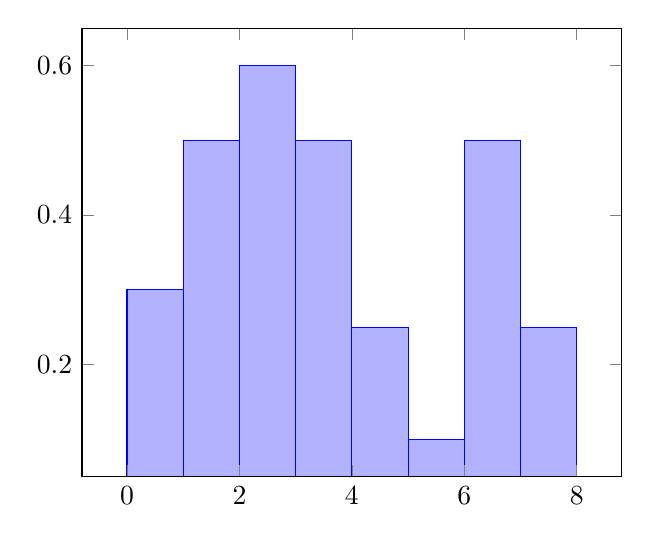
\begin{tikzpicture}
    \begin{axis}[area style]
        \addplot+[ybar interval,mark=no] plot coordinates {
                (0,.3)
                (1,.5)
                (2,.6)
                (3,.5)
                (4,.25)
                (5,.1)
                (6,.5)
                (7,.25)
                (8,.1)
            };
    \end{axis}
\end{tikzpicture}

\hfill \break
Das Kreisdiagramm:\\
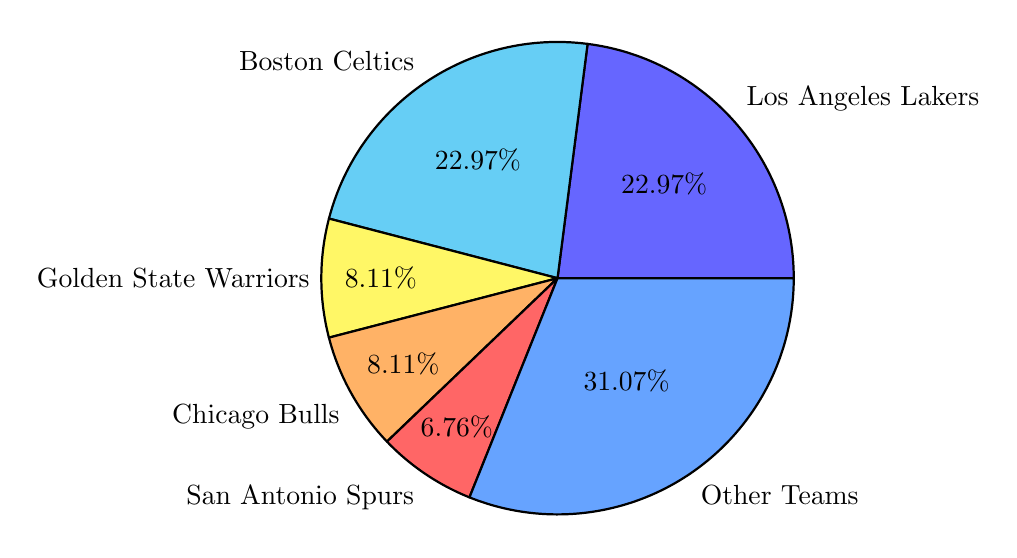
\begin{tikzpicture}
    \pie{22.97/Los Angeles Lakers,
        22.97/Boston Celtics,
        8.11/Golden State Warriors,
        8.11/Chicago Bulls,
        6.76/San Antonio Spurs,
        31.07/Other Teams}
\end{tikzpicture}
\hfill \break
\newpage
\subsection{Box Plot}

In einem Wald wurden die Stammumfänge von 120 Bäumen vermessen (Umfang in cm). Die Daten sind hier in Form eines Diagramms dargestellt.

\hfill \break
\begin{center}
\resizebox{10cm}{5cm}{%
    \begin{tikzpicture}
        \begin{axis}
            [
                ytick={1},
                yticklabels={},
            ]
            \addplot+[
                boxplot prepared={
                        median=48,
                        upper quartile=60,
                        lower quartile=45,
                        upper whisker=67,
                        lower whisker=30
                    },
            ] coordinates {};
        \end{axis}
    \end{tikzpicture}
}

\hfill \break
\begin{itemize}
    \item ca. $75\%$ der Bäume einen Stammumfang kleiner als 60cm haben.
    \item alle Bäume einen Stammumfang von höchstens 67cm haben.
    \item von den 120 Bäumen ca. 3O einen Stammumfang von höchstens 45cm haben.
    \item ca.: 60 Bäume einen Stammumfang von 45 bis 60 cm haben
\end{itemize}
\end{center}
\break
\newpage
\section{Lineare regression}

Mit Hilfe einer Regression können aus Messwerten Zusammenhänge (Korrelationen) gefunden werden.
Dazu braucht man (mindestens) zwei Größen, zwischen welchen ein Zusammenhang vermutet wird, und geeignete Wertepaare.

\hfill \break
Beispiel:\\
Es kann von jedem Teilnehmer eines BRP-Kurses die Entfernung seines Wohnortes vom Kursort (Liste 1) und die Zeit (Liste 2), die er dafür benötigt, notiert werden.
Man kann vermuten, dass zwischen diesem Weg und dieser Zeit ein Zusammenhang besteht.

\hfill \break
Taschenrechner:\\
\begin{itemize}
    \item Stat 
    \item $\rightarrow$
    \item Edit
    \item Liste L1 und L2 eingeben 
    \item Stat 
    \item $\rightarrow$
    \item Calc
    \item Linreg: L1,L2
\end{itemize}

\newpage
\hfill \break
Wie gut passt ein lineares Modell?\\
Für eine lineare Regression gibt es eine Größe, die angibt, wie gut das Lineare Modell passt.
Das ist der Korrelationskoeffizient (nach Pearson) r.
Sein Wert liegt immer zwischen -1 und 1. Er gibt an, ob ein linearer Zusammenhang vermutet werden kann, besteht oder eher ausgeschlossen werden kann.
Ob die Größen einander wirklich beeinflussen, kann aber nie mit Sicherheit bestimmt werden.

\hfill \break
\begin{itemize}
    \item $|r|\approx 1$ Ist der Betrag des Korrelationskoeffizienten nahe bei 1, so passt das lineare Modell sehr gut.
    \item $|r|\approx 0$ Ist der Korrelationskoeffizient sehr klein, nahe bei 0, so liegt vermutlich kein linearer Zusammenhang vor.
    \item $r > 0$ Ist der Korrelationskoeffizient positiv, so ist die Trendgerade steigend. Man spricht von einer positiven Korrelation.
    Wenn der Wert einer Größe zunimmt, so steigt auch der Wert der anderen Größe. (z.B.: Wer eine längere Strecke zurücklegen muss, braucht auch mehr Zeit.)
    \item Ist der Korrelationskoeffizient negativ, so ist die Trendgerade fallend. Man spricht von einer negativen Korrelation.
    Wenn der Wert einer Größe zunimmt, so sinkt der Wert der anderen Größe. (z.B.: Wenn der Preis eines Produktes steigt, so wird die verkaufte Menge sinken.)
    \item $r = 1$ oder $r=0$ Erreicht der Korrelationskoeffizient die Werte 1 oder -1 exakt, so handelt es sich um eine vollkommene Korrelation.
    Das heißt, dass man nicht eine möglichst gute Gerade gefunden hat, sondern dass alle Punkte exakt auf dieser Geraden liegen.
\end{itemize}

\hfill \break
Am Taschenrechner erhält man den Korrelationskoeffizienten automatisch bei der Berechnung der linearen Regression, wenn er aktiviert wurde.
Um dies zu tun braucht man aus dem Catalog (2nd: 0) den Befehl DiagnosticOn.
Wird dieser ausgewählt und mit Enter bestätigt, wird in weiterer Folge immer der Korrelationskoeffizient automatisch mitberechnet.
(Auch wenn der Taschenrechner zwischendurch ausgeschaltet wird, bleibt die Aktivierung erhalten.)


\newpage
\hfill \break
Gibt es nur lineare Trendlinien?\\
Als Modelle für Regressionen eignen sich verschieden Funktionstypen.
Zur Anwendung kommen insbesondere Polynomfunktionen bis zum Grad 4 und Logarithmus- und Exponentialfunktionen.
Den Korrelationskoeffizienten nach Pearson gibt es allerdings nur bei einer linearen Regression.

\hfill \break
Hier sieht man verschiedene Trendlinien für die gleichen Wertepaare.
Zuerst wurde eine Polynomfunktion 3. Grades als Modell gewählt.
Anschließend eine Exponentialfunktion und zum Schluss eine Logarithmusfunktion.
\break
\section{Vektor}

\hfill \break
\subsection{Was sind Vektoren?}

Ein Vektor hat drei Eigenschaften:\\
\begin{itemize}
    \item Richtung
    \item Betrag/Länge
    \item Orientierung
\end{itemize}
Dadurch wird er grafisch als Pfeil dargestellt. Die Richtung wird durch die (Schräg-) Lage des Pfeils festgelegt.
Sein Betrag entspricht der Länge des Pfeils. Die Orientierung ergibt sich daraus, an welchem Ende des Pfeils die Spitze liegt.
Die Position eines Vektors spielt keine Rolle.

\hfill \break
Diese drei Pfeile stellen immer den gleichen Vektor dar, weil die Richtung, die Länge und die Orientierung bei allen gleich sind.

\begin{tikzpicture}
    \draw[thin,gray!40] (-2,-2) grid (2,2);
    \draw[<->] (-2,0)--(2,0) node[right]{$x$};
    \draw[<->] (0,-2)--(0,2) node[above]{$y$};
    \draw[line width=2pt,red,-stealth](-2,-1)--(-1,1) node[anchor=south west]{};
    \draw[line width=1pt,blue,-stealth](-1,-2)--(0,0) node[anchor=south west]{};
    \draw[line width=2pt,green,-stealth](1,0)--(2,2) node[anchor=south west]{};
\end{tikzpicture}

\break
Diese beiden Vektoren haben die gleiche Richtung und den gleichen Betrag.
Sie unterscheiden sich nur in ihrer Orientierung. Sie sind zueinander die Gegenvektoren.

\begin{tikzpicture}
    \draw[thin,gray!40] (-2,-2) grid (2,2);
    \draw[<->] (-2,0)--(2,0) node[right]{$x$};
    \draw[<->] (0,-2)--(0,2) node[above]{$y$};
    \draw[line width=2pt,red,-stealth](-1,-1)--(0,1) node[anchor=south west]{};
    \draw[line width=2pt,blue,-stealth](1,1)--(0,-1) node[anchor=north east]{};
\end{tikzpicture}


\hfill \break
Für die Berechnung werden Vektoren ähnlich wie beim Steigungsdreieck von linearen Funktionen durch Komponenten entlang der Achsen dargestellt.

\hfill \break
Daher können Vektoren immer als Zahlenpaare dargestellt werden.
(Es gibt auch Vektoren im Raum, die mit 3 Komponenten dargestellt werden.)
Ob das Dreieck über oder unter dem Vektor gezeichnet wird, spielt keine Rolle.\\
$$\vec{a} = \binom{a_1}{a_2}$$
\hfill \break
\newpage
\subsection{Wie entstehen Vektoren? Wozu dienen Vektoren?}

\hfill \break
Vektoren können Wege beschreiben, wie man von einem Punkt zu einem anderen gelangt, wie bei einer Schatzkarte (3 Schritte nach Ost und 4 Schritte nach Nord).
Dazu verwendet man die Koordinaten der Punkte und subtrahiert die des Anfangspunktes vom Endpunkt (Spitze - Schaft).

\hfill \break
Verwendet man die Punkte in Vektorschreibweise, so nennt man sie Ortsvektoren.
Sie entsprechen der Verbindung vom Ursprung zum Punkt.

\hfill \break
Vektoren können auch physikalische Größen beschreiben, die eine Richtung aufweisen. Dabei kann es sich z.B. um
Geschwindigkeiten handeln oder Kräfte.

\hfill \break
Der Vektor $\vec{v}$ beschreibt eine Geschwindigkeit in Richtung Nordost.
Die Länge des Vektors entspricht dabei der Betrag der Geschwindigkeit.
Je länger der Vektor, desto größer die Geschwindigkeit.

\hfill \break
Die Vektoren $\vec{F_1}$ und $\vec{F_2}$ können Kräfte beschreiben, die zwei Freunde beim Seilziehen aufwenden.
(Sie ziehen entgegen-gesetzt.) Wieder gilt, je größer die Kraft, desto länger der Vektor.
Daher wird der mit der Kraft $\vec{F_1}$gewinnen.

\hfill \break
Vektoren können auch allgemeine Größen darstellen:\\
\begin{itemize}
    \item X ... Anzahl der gekauften Kuchen
    \item Y ... Anzahl der gekauften Torten
\end{itemize}
Der Vektor $\vec{s}$ besagt daher, dass 3 Kuchen und 5 Torten gekauft wurden.
Bei Vektor $\vec{t}$ sind es 4 Kuchen und eine Torte.
\hfill \break
\newpage
\subsection{Wie kann die Länge eines Vektors berechnet werden?}

\hfill \break
Die Länge (den Betrag) eines Vektors $\vec{a} = \binom{a_1}{a_2} $ erhalt man mit Hilfe des Satzes von Pythagoras. $|\vec{a}| = \sqrt{a_1^2+a_2^2}$

\hfill \break
Bei einem Vektor, der zwei Punkte verbindet, erhält man dadurch deren Entfernung (z.B.: 5 m oder 5 cm).
Bei Geschwindigkeiten oder Kräften erhält man ihren Betrag oder Wert (z.B.: 5 m/s oder 5 Newton).

\hfill \break
Die Länge eines Vektors kann man verändern, indem man ihn mit einem Skalar (= Zahl) multipliziert.
Man erhält dadurch parallele Vektoren, weil sie die gleiche Richtung haben.
$$k+\vec{a}=k*\binom{a_1}{a_2} = \binom{k*a_1}{k*a_2}$$

\hfill \break
Der Vektor $\vec{b}$ ist doppelt so lang wie der Vektor $\vec{a}$, hat aber die selbe Richtung und Orientierung.

\hfill \break
Soll die Orientierung des Vektors geändert werden, so multipliziert man ihn mit einer negativen Zahl.
Der Vektor $\vec{c}$ hat die selbe Richtung und Länge wie der Vektor $\vec{a}$, aber eine andere Orientierung.
Daher heißt er Gegenvektor des Vektors $\vec{a}$.

\hfill \break
Sucht man den Einheitsvektor, so sucht man einen Vektor mit der gleichen Richtung und Orientierung, aber mit der Länge 1.
Ihn erhält man, indem man den ursprünglichen Vektor durch seine Länge dividiert, oder mit dem Kehrwert seiner Länge multipliziert.
$$\vec{a_0}  = \frac{1}{|\vec{a}|}*\vec{a}$$

\hfill \break
Mit Einheitsvektoren kann man auch bestimmen, wie lange ein Vektor sein soll.
Hat er nämlich schon Länge 1, braucht er nur noch mit der gewünschten Länge multipliziert werden.
\hfill \break
\newpage
\subsection{Wie kann man mit Vektoren rechnen?}

\hfill \break
Wenn man zwei Vektoren $\vec{a} ? \binom{a_1}{a_2}$ und $\vec{b} ? \binom{b_1}{b_2}$ addiert, so hängt man sie einfach hintereinander.
$$\vec{a}+\vec{b} = \binom{a_1}{a_2} + \binom{b_1}{b_2} = \binom{a_1+b_1}{a_2+b_2}$$

\hfill \break
Wenn es sich um Entfernungen zweier Punkte handelt, so geht man (auf der Schatzkarte) beide Wege bzw. als Summe den direkten Weg.

\hfill \break
Handelt es sich um physikalische Größen, so bildet man den resultierenden Vektor.
Man erhält ihn durch ein Parallelogramm. Man erhält dasselbe Ergebnis wie in ersterem Fall.
Wenn beide Kräfte $\vec{F_1}$ und $\vec{F_2}$ wirken, so kann man sie beide durch die resultierende Kraft $\vec{F}$ ersetzen.
Sie hat die gleiche Wirkung, wie die beiden anderen Kräfte zusammen. (Kräfteparallelogramm)

\hfill \break
Subtrahiert man einen Vektor, so wird eigentlich sein Gegenvektor addiert.
$$\vec{a} - \vec{b} = \binom{2}{4}-\binom{5}{2} = \binom{2}{4} + \binom{-5}{-2}-\binom{-3}{2}$$

\hfill \break
Beim Addieren von zwei Vektoren entsteht immer ein neuer Vektor. Dieser kann länger oder auch kürzer als die einzelnen ursprünglichen Vektoren sein.
\begin{itemize}
    \item Wenn man zwei Wege hintereinander geht, hätte man auch eine Abkürzung statt dessen gehen können und der Weg wäre kürzer gewesen.
    \item Wenn Kräfte nicht in die gleiche Richtung wirken, sondern gegeneinander, so wird die resultierende Kraft kleiner sein.
\end{itemize}

\hfill \break
Für allgemeine Größen ist die Addition von Vektoren ideal, weil mehrere Werte gleichzeitig addiert werden können.
\hfill \break
\newpage
\subsection{Wie kann die Lage von Vektoren bestimmt werden?}

\hfill \break
Vektoren können auch multipliziert werden.
Bildet man das Skalarprodukt zweier Vektoren $\vec{a} = \binom{a_1}{a_2}$ und $\vec{b} = \binom{b_1}{b_2}$, so ist das Ergebnis ein Skalar (eine Zahl).
$$\vec{a} * \vec{b} = \binom{a_1}{a_2} * \binom{b_1}{b_2} = a_1 * b_1 + a_2 * b_2$$

\hfill \break
Beim Skalarprodukt wird einer der Vektoren auf den anderen "normal" projiziert.
Hier sieht man, wie der Vektor $\vec{d}$ auf den Vektor $\vec{a}$ projiziert wird.
Es ergibt sich der Vektor $\vec{b_a}$.
Das Skalarprodukt berechnet dann das Produkt der Längen von $\vec{a}$ und von $\vec{b_a}$.\\
Verwendet wird das Skalarprodukt, wenn man die Lage von Vektoren zueinander untersuchen möchte.

\hfill \break
Das Skalarprodukt von Vektoren, die normal aufeinander stehen, ist 0.
(Die Projektion liefert einen Vektor mit Länge 0.)
$$\vec{c} * \vec{d} = \binom{4}{2} * \binom{1}{-2} = 4 * 1 + 2 * (-2) = 0$$

\hfill \break
Skalarprodukte können positiv oder negativ sein, das liegt an dem Winkel, den die Vektoren miteinander einschließen.
Bei einem negativen Ergebnis ist der Winkel stumpf, bei einem positiven Ergebnis ist er spitz. Ist das Ergebnis O ist der Winkel 90°.

\hfill \break
\begin{itemize}
    \item $\vec{e} = \binom{3}{-2}$
    \item $\vec{f} = \binom{-1}{3}$
    \item $\vec{g} = \binom{4}{6}$
\end{itemize}

\hfill \break
$$\vec{e} * \vec{f} = 3 * (-1) + (-2) * 3 = -9$$
$$\vec{e}*\vec{f} = 3 * 4 + (-2) * 6 = 0$$
$$\vec{f} * \vec{g} = (-1) * 4 + 3 * 6 = 14$$
\break
\newpage
\section{Kostenrechnung}

\hfill \break
Kostenfuntion:
\begin{itemize}
    \item Lineare Kostenfuntion: $K(x)=30x+\textcolor{green}{2500}$
    \item Quadratische Kostenfuntion: $K(x)=0.0.x^2+120x+\textcolor{green}{12800}$
    \item Kostenfuntion 3.Grades: $K(x)=-0.05x^3+7.775x^2+-10.31x+\textcolor{green}{5000}$
\end{itemize}

\begin{itemize}
    \item $\textcolor{green}{Zusatzkosten}$
\end{itemize}


\hfill \break
Der Wendepunkt in einer Kostenrechnung wird Kostenkeere gennnat.
\begin{itemize}
    \item bis zu diesem Punkt: Degresive Kosten
    \item ab dem Punkt: Progresive Kosten
\end{itemize}

\hfill \break
Duchschnittliche Kosten pro Stück: $\frac{K(x)}{x}$\\

\hfill \break
Erlösfunktion (Umsatz): $E(x) = \textcolor{red}{p}*\textcolor{blue}{t}$\\
\begin{itemize}
    \item $\textcolor{red}{p}$ = Verkaufspreis
    \item $\textcolor{blue}{t}$ = Stück
\end{itemize}

\hfill \break
Gewinnfuntion: $G(x) = E(x)-K(x)$\\
$G(x)=0$ = Break even point / Gewinnschwelle

\hfill \break
Nachfragefuntion: $n(x) = -1.5x+360$\\
Preisefuntion: $p(x) = \frac{E(x)}{x}$

\hfill \break
Sättigungsmenge: Jene Stückzahl wo der Preisen gleich 0 ist. (Markt ist Gesättigt)\\
Hüchstpreich: Jener Preis bei dem kein eiziges Stück mehr verkauft wird.
\break
\newpage
\section{Folgen und Reihen}

Ordnet man jeder natürlichen Zahl $n \in \mathbb{N}$ eine reelle Zahl $a_{\mathrm{n}}$ eindeutig zu, so entsteht eine unendliche (reelle) Folge $(a_{\mathrm{n}})$.
Die einzelnen Werte der Folge heißen Folgenglieder und werden mit Indizes durchnummeriert:

$$( a_{\mathrm{n}} ) = a_1 ,\,  a_2 ,\, a_3 ,\, \ldots,\, a_{\mathrm{n}} ,\, \ldots$$

Im Unterschied zu einer Menge kann bei einer Folge ein und das selbe Glied mehrere Male auftreten.
Die Definition einer Folge kann auf zweierlei Arten erfolgen:

Viele Folgen lassen sich nach einem Bildungsgesetz mittels eines Terms aufstellen. Das Bildungsgesetz wird hierzu in runde Klammern geschrieben.
Beispiel:

$$(a_{\mathrm{n}}) = (2 \cdot n^2) = 2 ,\,  8 ,\,  18 ,\, 32 ,\, \ldots$$

Ist (mindestens) das erste Folgenglied bekannt und besteht eine Rechenvorschrift, wie sich ein Folgenglied aus einem vorhergehenden berechnen lässt, so sind alle Glieder einer Folge ebenfalls eindeutig festgelegt.
Dieses Vorgehen wird als Rekursion bezeichnet. Beispiel:

$$a_{\mathrm{n}} = 0 ,\, 1 ,\, 2 ,\, 3 ,\, 5 ,\, 8 ,\, 13 ,\, 21 ,\, \ldots$$

Die obige Zahlenfolge wird auch zu Ehren von Leonardo Fibonacci als Fibonacci-Folge bezeichnet.
Die Folgenglieder lassen sich dadurch berechnen, indem jeweils die Summe der beiden vorangehenden Folgenglieder gebildet wird.
Das Bildungsgesetz der Folge lautet somit für $n \ge 2$:

$$a_{\mathrm{n}} = a_{\mathrm{n-2}} + a_{\mathrm{n-1}}$$

Beschränkt man die Definitionsmenge auf die ersten n natürlichen Zahlen $(n \ne 0)$, so erhält man eine endliche Folge mit dem Anfangsglied $a_1$ und dem Endglied $a_{\mathrm{n}}$.


\hfill \break
\newpage
\subsection{Arithmetische Folgen}

Eine Folge heißt arithmetisch, wenn die Differenz d zweier aufeinander folgender Glieder stets konstant ist.
Für eine arithmetische Folge gilt also:

$$a_{\mathrm{n + 1}} - a_{\mathrm{n}} = d$$

Als Bildungsgesetz gilt:

$$a_{\mathrm{n}} =  a_1 + (n - 1) \cdot d$$

Ist $d > 0$, so ist die Folge (streng) monoton steigend, bei $d < 0$ ist die Folge (streng) monoton fallend. Gilt $d=0$, so ist die Folge konstant.

Da die einzelnen Folgenglieder immer um den gleichen Betrag zu- beziehungsweise abnehmen, ist das mittlere dreier Folgenglieder stets gleich dem arithmetischen Mittel der beiden benachbarten Folgenglieder.
Es gilt also:

$$a_{\mathrm{n}} = \frac{a_{\mathrm{n + 1}} + a_{\mathrm{n-1}}}{2}$$

Wichtige arithmetische Folgen sind beispielsweise die natürlichen Zahlen $1 ,\, 2 ,\, 3 ,\, 4 ,\, \ldots$,
die geraden Zahlen $2 ,\, 4 ,\, 6 ,\, 8 ,\, \ldots$, die ungeraden Zahlen $1 ,\, 3 ,\, 5 ,\, 7 ,\,\ldots$, usw.

Will man zwischen zwei Werten $a_1$ und $a_2$ insgesamt $n$ weitere Zahlen als eine arithmetische Folge einfügen, so gilt dabei für alle Differenzen der einzelnen Folgenglieder:

$$d_{\mathrm{i}} = \frac{a_2 - a_1}{n + 1}$$

Diese Formel kann beispielsweise hilfreich sein, um fehlende Werte in Wertetabellen (näherungsweise) zu ergänzen.
Eine ähnliche Anwendung kann darin bestehen, $n$ Objekte (beispielsweise Holzbalken) in jeweils gleichem Abstand voneinander zwischen zwei festen Grenzen $a_1$ und $a_2$ einzufügen; dabei gibt $d_{\mathrm{i}}$ an, in welchem Abstand die Mittelpunkte der Objekte jeweils eingefügt werden müssen.
\hfill \break
\newpage
\subsection{Geometrische Folgen}

Eine Folge heißt geometrisch, wenn der Quotient $q$ zweier aufeinander folgender Glieder stets konstant ist.
Für eine jede geometrische Folge gilt also:

$$\frac{a_{\mathrm{n + 1}}}{ a_{\mathrm{n}} } = q$$

Als Bildungsgesetz gilt:

$$a_{\mathrm{n}} =  a_1 \cdot q ^{n-1}$$

Ist $q > 1$, so ist die Folge (streng) monoton zunehmend, bei $0 < q< 1$ ist die Folge (streng) monoton abnehmend und konvergiert gegen Null.
Gilt $q=0$, so ist die Folge konstant, im Fall - $\infty < q < 0$ ist die Folge alternierend, die Werte der Folgenglieder sind also abwechselnd positiv und negativ.

Da die einzelnen Folgenglieder immer um den gleichen Faktor zu- beziehungsweise abnehmen, ist das mittlere dreier Folgenglieder stets gleich dem geometrischen Mittel der beiden benachbarten Folgenglieder. Es gilt also:[2]

$$| a_{\mathrm{n}} | = \sqrt{a_{\mathrm{n+1}} \cdot a_{\mathrm{n-1}}}$$

Will man zwischen zwei Werten $a_1$ und $a_2$ insgesamt n weitere Zahlen als eine geometrische Folge einfügen, so gilt dabei für alle Quotienten der einzelnen Folgenglieder:

$$q_{\mathrm{i}} = \sqrt[n+1]{\frac{ a_2}{ a_1}}$$

\end{document}
